%%%%%%%%%%%%%%%%%%%%%%%%%%%%%%%%%%%%%%%%%
% Wenneker Article LaTeX Template Version 2.0 (28/2/17)
%
% This template was downloaded from: http://www.LaTeXTemplates.com
%
% Authors: Vel (vel@LaTeXTemplates.com) Frits Wenneker
%
% License: CC BY-NC-SA 3.0 (http://creativecommons.org/licenses/by-nc-sa/3.0/)
%
%%%%%%%%%%%%%%%%%%%%%%%%%%%%%%%%%%%%%%%%%

%----------------------------------------------------------------------------------------
%	PACKAGES AND OTHER DOCUMENT CONFIGURATIONS
%----------------------------------------------------------------------------------------

\documentclass[10pt, a4paper]{report} % 10pt font size (11 and 12 also possible), A4 paper (letterpaper for US letter)

%%%%%%%%%%%%%%%%%%%%%%%%%%%%%%%%%%%%%%%%%
% Wenneker Article
% Structure Specification File
% Version 1.0 (28/2/17)
%
% This file originates from:
% http://www.LaTeXTemplates.com
%
% Authors:
% Frits Wenneker
% Vel (vel@LaTeXTemplates.com)
%
% License:
% CC BY-NC-SA 3.0 (http://creativecommons.org/licenses/by-nc-sa/3.0/)
%
%%%%%%%%%%%%%%%%%%%%%%%%%%%%%%%%%%%%%%%%%

%----------------------------------------------------------------------------------------
%	PACKAGES AND OTHER DOCUMENT CONFIGURATIONS
%----------------------------------------------------------------------------------------

\usepackage[english]{babel} % English language hyphenation

\usepackage{microtype} % Better typography

\usepackage{amsmath,amsfonts,amsthm} % Math packages for equations

\usepackage[svgnames]{xcolor} % Enabling colors by their 'svgnames'

\usepackage[hang, small, labelfont=bf, up, textfont=it]{caption} % Custom captions under/above tables and figures

\usepackage{booktabs} % Horizontal rules in tables

\usepackage{lastpage} % Used to determine the number of pages in the document (for "Page X of Total")

\usepackage{graphicx} % Required for adding images

\usepackage{enumitem} % Required for customising lists
\setlist{noitemsep} % Remove spacing between bullet/numbered list elements

\usepackage{sectsty} % Enables custom section titles
\allsectionsfont{\usefont{OT1}{phv}{b}{n}} % Change the font of all section commands (Helvetica)

\usepackage{amsmath} % Allows for mathematical symbols
\usepackage{mdframed} % Allows for framing of text

%----------------------------------------------------------------------------------------
%	MARGINS AND SPACING
%----------------------------------------------------------------------------------------

\usepackage{geometry} % Required for adjusting page dimensions

\geometry{
	top=1cm, % Top margin
	bottom=1.5cm, % Bottom margin
	left=2cm, % Left margin
	right=2cm, % Right margin
	includehead, % Include space for a header
	includefoot, % Include space for a footer
	%showframe, % Uncomment to show how the type block is set on the page
}

\setlength{\columnsep}{2.5mm} % Column separation width

\setlength{\parskip}{2.5mm} % Increase spacing between paragraphs

%----------------------------------------------------------------------------------------
%	FONTS
%----------------------------------------------------------------------------------------

\usepackage[T1]{fontenc} % Output font encoding for international characters
\usepackage[utf8]{inputenc} % Required for inputting international characters

\usepackage{XCharter} % Use the XCharter font

%----------------------------------------------------------------------------------------
%	HEADERS AND FOOTERS
%----------------------------------------------------------------------------------------

\usepackage{fancyhdr} % Needed to define custom headers/footers
\pagestyle{fancy} % Enables the custom headers/footers

\renewcommand{\headrulewidth}{0.0pt} % No header rule
\renewcommand{\footrulewidth}{0.4pt} % Thin footer rule

\renewcommand{\sectionmark}[1]{\markboth{#1}{}} % Removes the section number from the header when \leftmark is used

%\nouppercase\leftmark % Add this to one of the lines below if you want a section title in the header/footer

% Headers
\lhead{} % Left header
\chead{\fontfamily{phv}\selectfont\textit{\thetitle}} % Center header - currently printing the article title
\rhead{} % Right header

% Footers
\lfoot{} % Left footer
\cfoot{} % Center footer
\rfoot{\fontfamily{phv}\selectfont\footnotesize Page \thepage\ of \pageref{LastPage}} % Right footer, "Page 1 of 2"

\fancypagestyle{firstpage}{ % Page style for the first page with the title
	\fancyhf{}
	\renewcommand{\footrulewidth}{0.0pt} % Suppress footer rule
}

\makeatletter{}
\renewcommand{\thepage}{\textsf{\@arabic\c@page}}
\makeatother{}

%----------------------------------------------------------------------------------------
%	TITLE SECTION
%----------------------------------------------------------------------------------------

\definecolor{tudublinblue}{HTML}{004C6C}

\newcommand{\authorstyle}[1]{{\large\usefont{OT1}{phv}{b}{n}\color{tudublinblue}#1}} % Authors style (Helvetica)

\newcommand{\institution}[1]{{\footnotesize\usefont{OT1}{phv}{m}{sl}\color{Black}#1}} % Institutions style (Helvetica)

\usepackage{titling} % Allows custom title configuration

\newcommand{\HorRule}{\color{DarkGrey}\rule{\linewidth}{1pt}} % Defines the gold horizontal rule around the title

\pretitle{
	\vspace{-30pt} % Move the entire title section up
	\HorRule\vspace{10pt} % Horizontal rule before the title
	\fontsize{32}{36}\usefont{OT1}{phv}{b}{n}\selectfont % Helvetica
	\color{tudublinblue} % Text colour for the title and author(s)
}

\posttitle{\par\vskip 15pt} % Whitespace under the title

\preauthor{} % Anything that will appear before \author is printed

\postauthor{ % Anything that will appear after \author is printed
	\vspace{10pt} % Space before the rule
	\par\HorRule % Horizontal rule after the title
	\vspace{20pt} % Space after the title section
}



%----------------------------------------------------------------------------------------
%	TABLE OF CONTENTS
%----------------------------------------------------------------------------------------

\usepackage{tocloft}



% fonts for TOC
\renewcommand{\cfttoctitlefont}{\fontfamily{phv}\selectfont\Large\bfseries}
\renewcommand{\cftsecfont}{\fontfamily{phv}\selectfont\bfseries}
\renewcommand{\cftsecpagefont}{\fontfamily{phv}\selectfont}
\renewcommand{\cftsubsecfont}{\fontfamily{phv}\selectfont\itshape}
\renewcommand{\cftsubsecpagefont}{\fontfamily{phv}\selectfont}

\renewcommand{\cftloftitlefont}{\fontfamily{phv}\selectfont\Large\bfseries} % List of Figures title
\renewcommand{\cftlottitlefont}{\fontfamily{phv}\selectfont\Large\bfseries} % List of Tables title

\setcounter{tocdepth}{3}


%----------------------------------------------------------------------------------------
%	ABSTRACT
%----------------------------------------------------------------------------------------

\usepackage{lettrine} % Package to accentuate the first letter of the text (lettrine)
\usepackage{fix-cm}	% Fixes the height of the lettrine

\newcommand{\initial}[1]{ % Defines the command and style for the lettrine
	\lettrine[lines=3,findent=4pt,nindent=0pt]{% Lettrine takes up 3 lines, the text to the right of it is indented 4pt and further indenting of lines 2+ is stopped
		\color{DarkGoldenrod}% Lettrine colour
		{#1}% The letter
	}{}%
}

\usepackage{xstring} % Required for string manipulation

\newcommand{\lettrineabstract}[1]{
	\StrLeft{#1}{1}[\firstletter] % Capture the first letter of the abstract for the lettrine
	\initial{\firstletter}\textbf{\StrGobbleLeft{#1}{1}} % Print the abstract with the first letter as a lettrine and the rest in bold
}

%----------------------------------------------------------------------------------------
%	BIBLIOGRAPHY
%----------------------------------------------------------------------------------------

\usepackage[backend=bibtex,style=authoryear,natbib=true]{biblatex} % Use the bibtex backend with the authoryear citation style (which resembles APA)

\addbibresource{sources.bib} % The filename of the bibliography

\usepackage[autostyle=true]{csquotes} % Required to generate language-dependent quotes in the bibliography
 % Specifies the document structure and loads requires packages

%----------------------------------------------------------------------------------------
%	ARTICLE INFORMATION
%----------------------------------------------------------------------------------------

\title{
  Final Report: \textit{Magpie -- Services at a Glance}
  } % The article title

\author{
    \authorstyle{
    \begin{tabular}{p{0.425\columnwidth} p{0.5\columnwidth} p{0.425\columnwidth} p{0.5\columnwidth}}
        Saul Burgess & C19349793 & Andreas Kraus & D23125112 \\
        Kaustubh Trivedi & D23124940 & Jessica Fornetti & D23124588 \\
        Anais Blenet & D22127697 & Yuanshuo Du & D22125495
    \end{tabular}
        } % Authors
}

% Example of a one line author/institution relationship
%\author{\newauthor{John Marston} \newinstitution{Universidad Nacional Autónoma de México, Mexico City, Mexico}}

\date{\today} % Add a date here if you would like one to appear underneath the title block, use \today for the current date, leave empty for no date

%----------------------------------------------------------------------------------------
\begin{document}

\begin{titlepage}
  \begin{center}
    {\Large\usefont{OT1}{phv}{b}{n}\color{tudublinblue}
      \includegraphics[width=0.5\textwidth]{images/TUDublin_Colour_RGB.png}

      \vspace{1cm}
      MSc in Computing \\
      Advanced Software Development \rule[-1mm]{1.5pt}{1.1em} Data Science \\
      \vspace{1cm}
      Team Project \\
      \vspace{1cm}
      Final Report \\

      \vspace{2.5cm}

      \Huge\textbf{Magpie} \\
      \vspace{0.25cm}
      \Large{Services at a Glance}

      \vspace{2.5cm}

      \Large{}
      Group 3 \\
      \vspace{0.25cm}
      \setlength\arrayrulewidth{1.5pt}
      \begin{tabular}{l l | l l}
        Saul Burgess     & C19349793 & Andreas Kraus    & D23125112  \\
        Kaustubh Trivedi & D23124940 & Jessica Fornetti & D23124588  \\
        Anais Blenet     & D22127697 & Yuanshuo Du      & D22125495
      \end{tabular}

      \vspace{2.5cm}

      \today{}
    }

  \end{center}
\end{titlepage}

\onecolumn{}
\pagenumbering{Roman}
\pagestyle{plain}

\newgeometry{left=2.5cm,top=2cm,right=2.5cm,bottom=2.5cm}

\makeatletter{}
\renewcommand{\tableofcontents}{
  \section*{Table of Contents} % Custom title
  \@starttoc{toc}
  }
\makeatother{}

\makeatletter{}
\renewcommand{\thepage}{\textsf{\Roman{page}}} % Sans-serif Roman numbers
\makeatother{}

\cleardoublepage{}
\addcontentsline{toc}{section}{Table of Contents}
\tableofcontents{}

\cleardoublepage{}
\addcontentsline{toc}{section}{List of Figures}
\listoffigures{}

\cleardoublepage{}
\addcontentsline{toc}{section}{List of Tables}
\listoftables{}

\cleardoublepage{}
\addcontentsline{toc}{section}{List of Listings}
\listoflistings{}

\restoregeometry{}
\pagenumbering{arabic}

%----------------------------------------------------------------------------------------
%	ARTICLE CONTENTS
%----------------------------------------------------------------------------------------

\onecolumn % Ensure single-column layout

\section{Introduction}
Urbanization brings increasing demands for efficient city planning and
sustainability. \textbf{Magpie – Services at a Glance} is a geographical
information service designed to address these challenges by offering a
streamlined platform for accessing and analysing public amenities. Developed as
part of the MSc in Computing (Advanced Software Development | Data Science)
group project, \textbf{Magpie} combines cutting-edge machine learning, intuitive
visualization, and robust data aggregation to provide a high-level overview of
public infrastructure.

Targeting urban planners \textbf{Magpie} simplifies the traditionally complex
and fragmented processes of data collection and analysis. By integrating
satellite imagery, automated detection techniques, and multi-layered data
visualization, the system identifies parking spots, bike infrastructure and more
-- all at a glance. Unlike existing tools that rely on manual input or advanced
GIS expertise, \textbf{Magpie} automates the extraction and fusion of real-world
data, ensuring accessibility and ease of use.

This report details the technical challenges, innovative solutions, and
real-world applications of \textbf{Magpie}. From the architecture and machine
learning methodologies to the user-centric frontend and robust backend
infrastructure, each component contributes to a powerful tool that empowers
informed decision-making and urban development.


\section{User Scenario}
\documentclass[preview]{standalone}
\begin{document}

\subsection{Who is our target user?}
\textit{Magpie's} primary target is Urban Planners. Urban Planners are
professionals responsible for the development of cities and towns, focusing on
the efficient use of land, infrastructure planning, and the creation of
sustainable and resilient communities. (\cite{fischler2012fifty}) Our secondary
target is any casual user who is interested in amenities planning, and this
includes but is not limited to the following: Sustainability Advocates,
Commuters, Event Planners, Journalists, Political Advisors, and Parking
Companies.

These personas were developed on basis of a combination of real-life people who
are known to our team, as well as based on research into the goals and needs of
people in these professions

\subsubsection{Primary Persona - Michael O'Brien}
O'Brien is a 48-year-old Urban Planning Specialist at Dublin City Council,
deeply committed to enhancing his hometown of Lusk. He specializes in
sustainable urban development, integrating smart technologies with traditional
planning principles, and has contributed to notable projects like Dublin's cycle
lane network. He represents our primary target user.

Michael is currently working on the expansion of Dublin's cycle lane network
southbound. He is facing some challenges because the maps provided by Dublin
city council are static and don't show crucial information such as public
facilities and amenities. The datasets he's been accessing seem out of date and
not comprehensive at all. Michael needs a tool that allows him to interact with
a map that contains key data on public facilities and amenities, as well as
options to extract that information for analysis and planning.

%michael user persona
\begin{figure}[htbp]
    \centering{}{}
    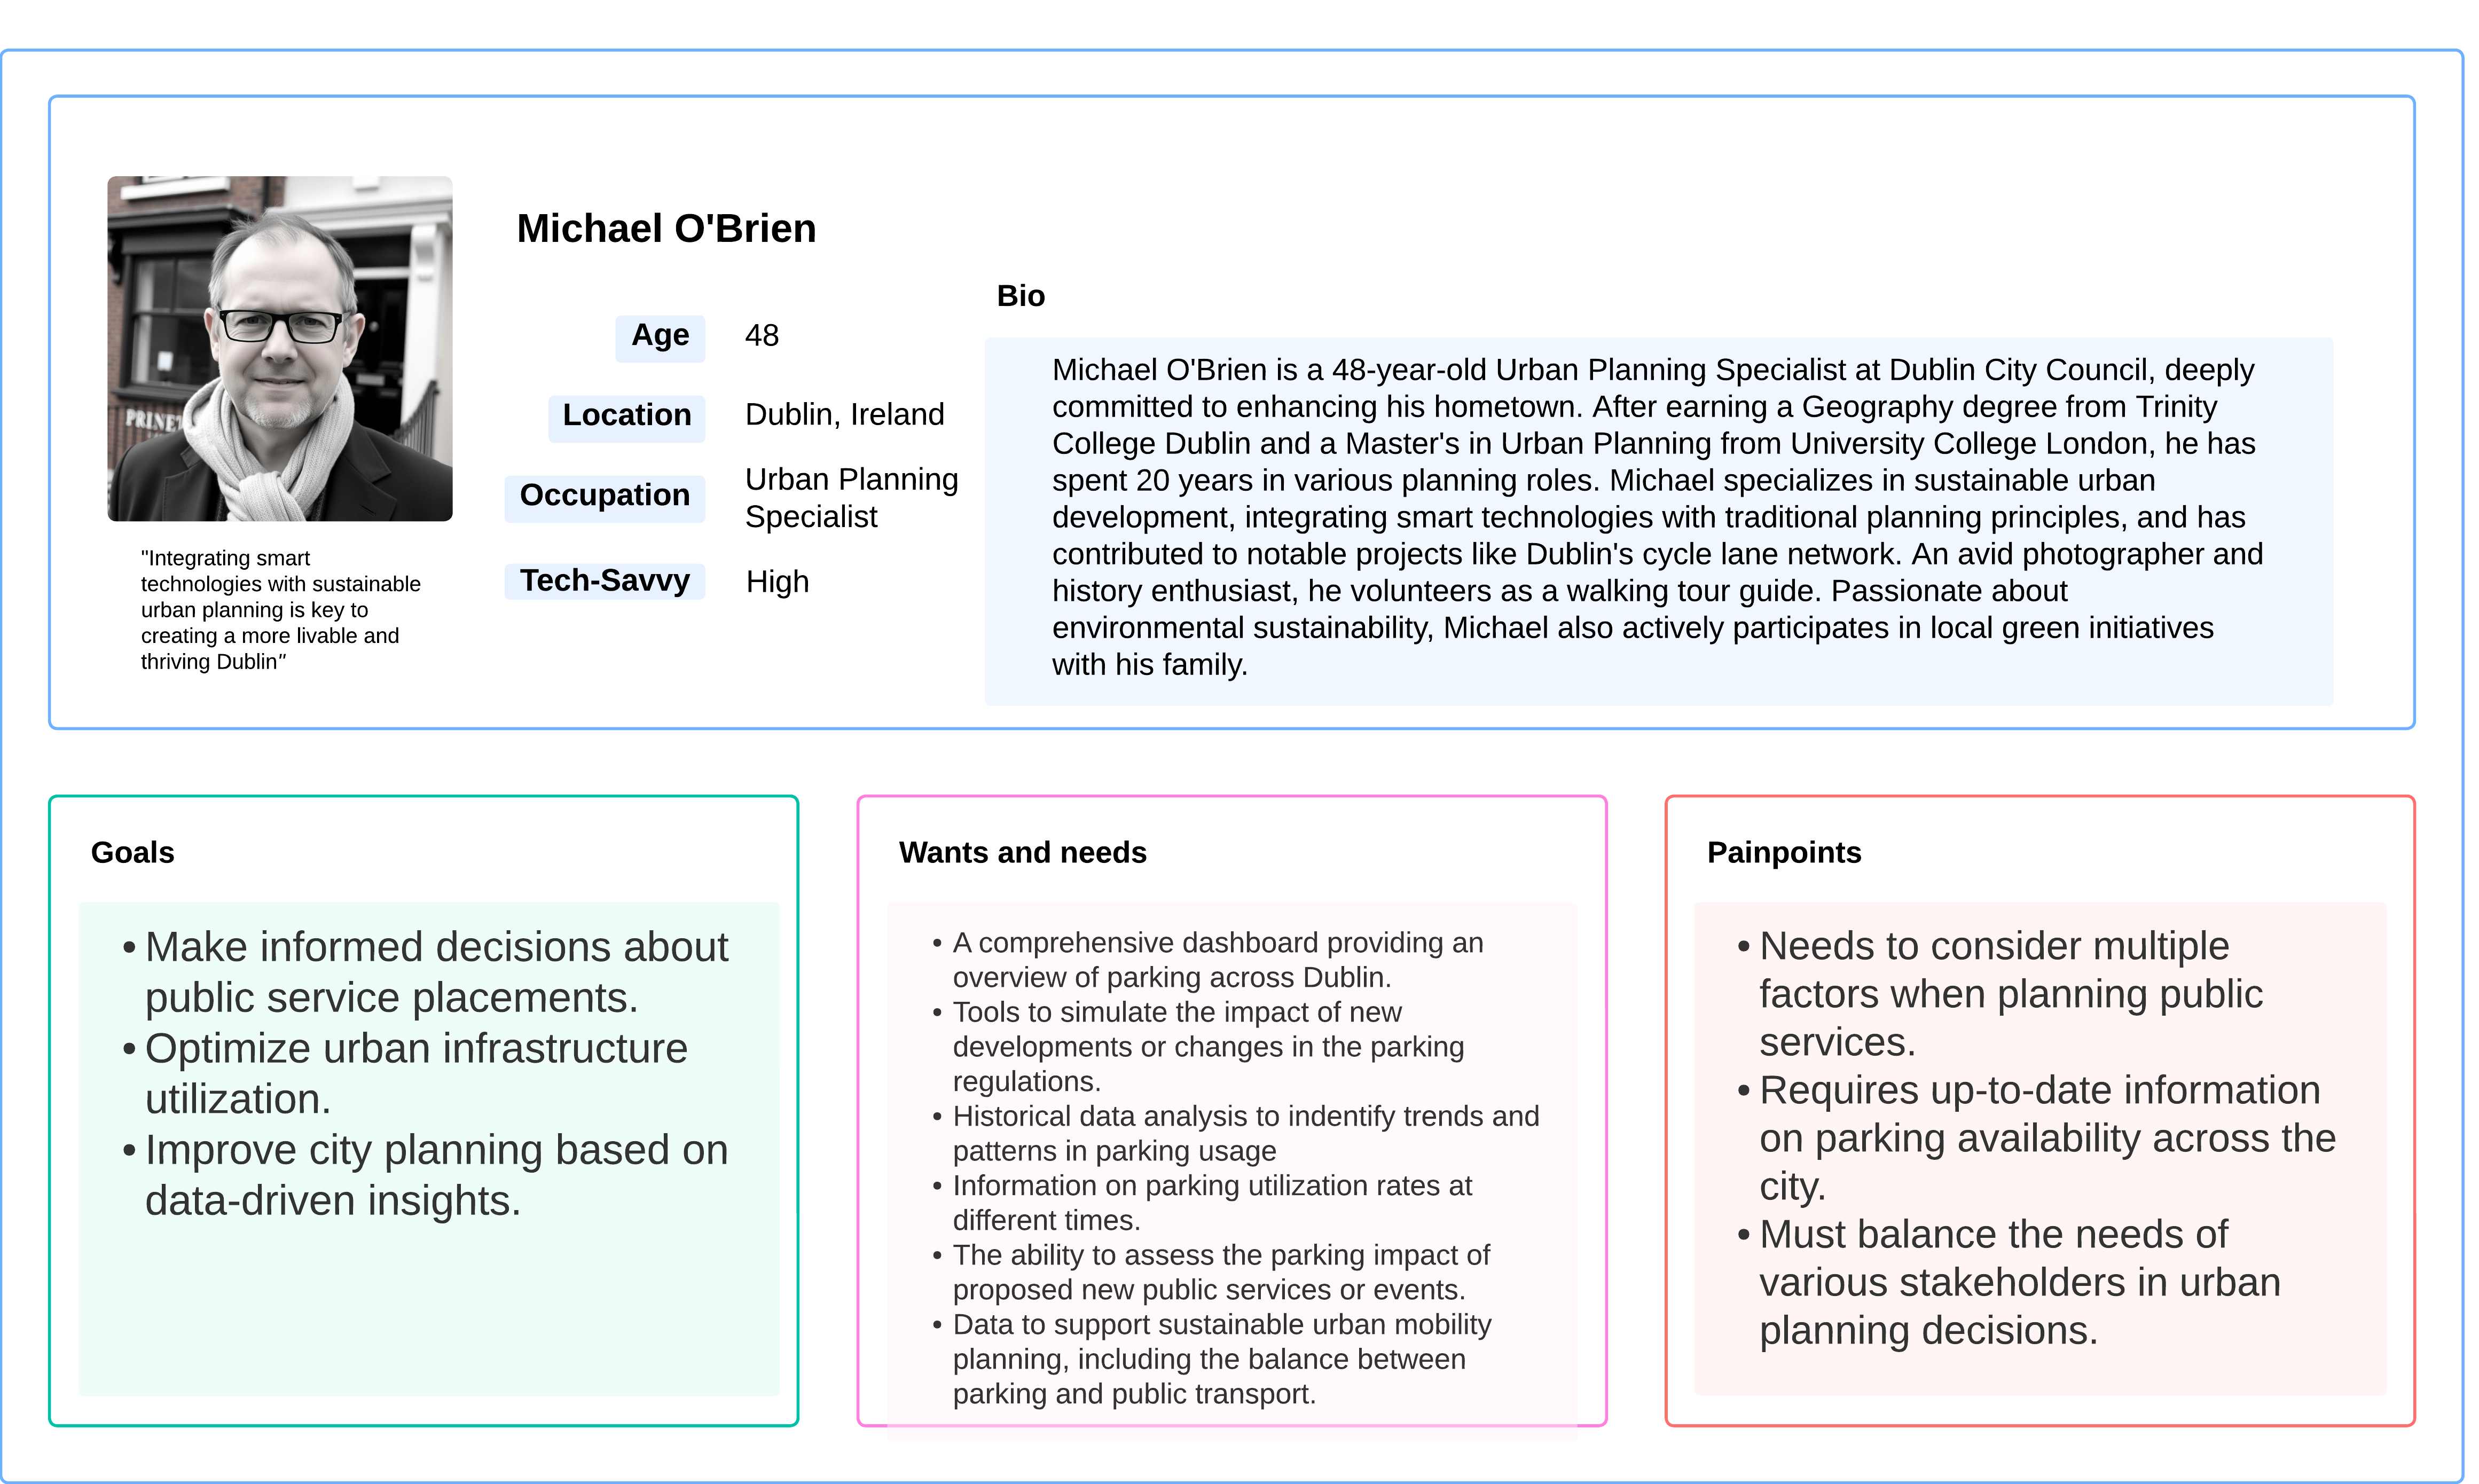
\includegraphics[width=0.8\textwidth]{images/michael-obrien-userpersona.png}
    \caption{User persona - Michael O'Brien}
\end{figure}

\subsubsection{Secondary Persona - Sarah Thompson}
Sarah thompson is a 35 year old CEO of an event's planning company based in
Dublin, Ireland. She specializes in corporate events and weddings, and is known
for creating memorable experiences while addressing key logistical challenges
such as venue selection, catering, accessibility and transportation. She
represents our secondary target user.

%sarah user persona
\begin{figure}[htbp!]
    \centering{}{}
    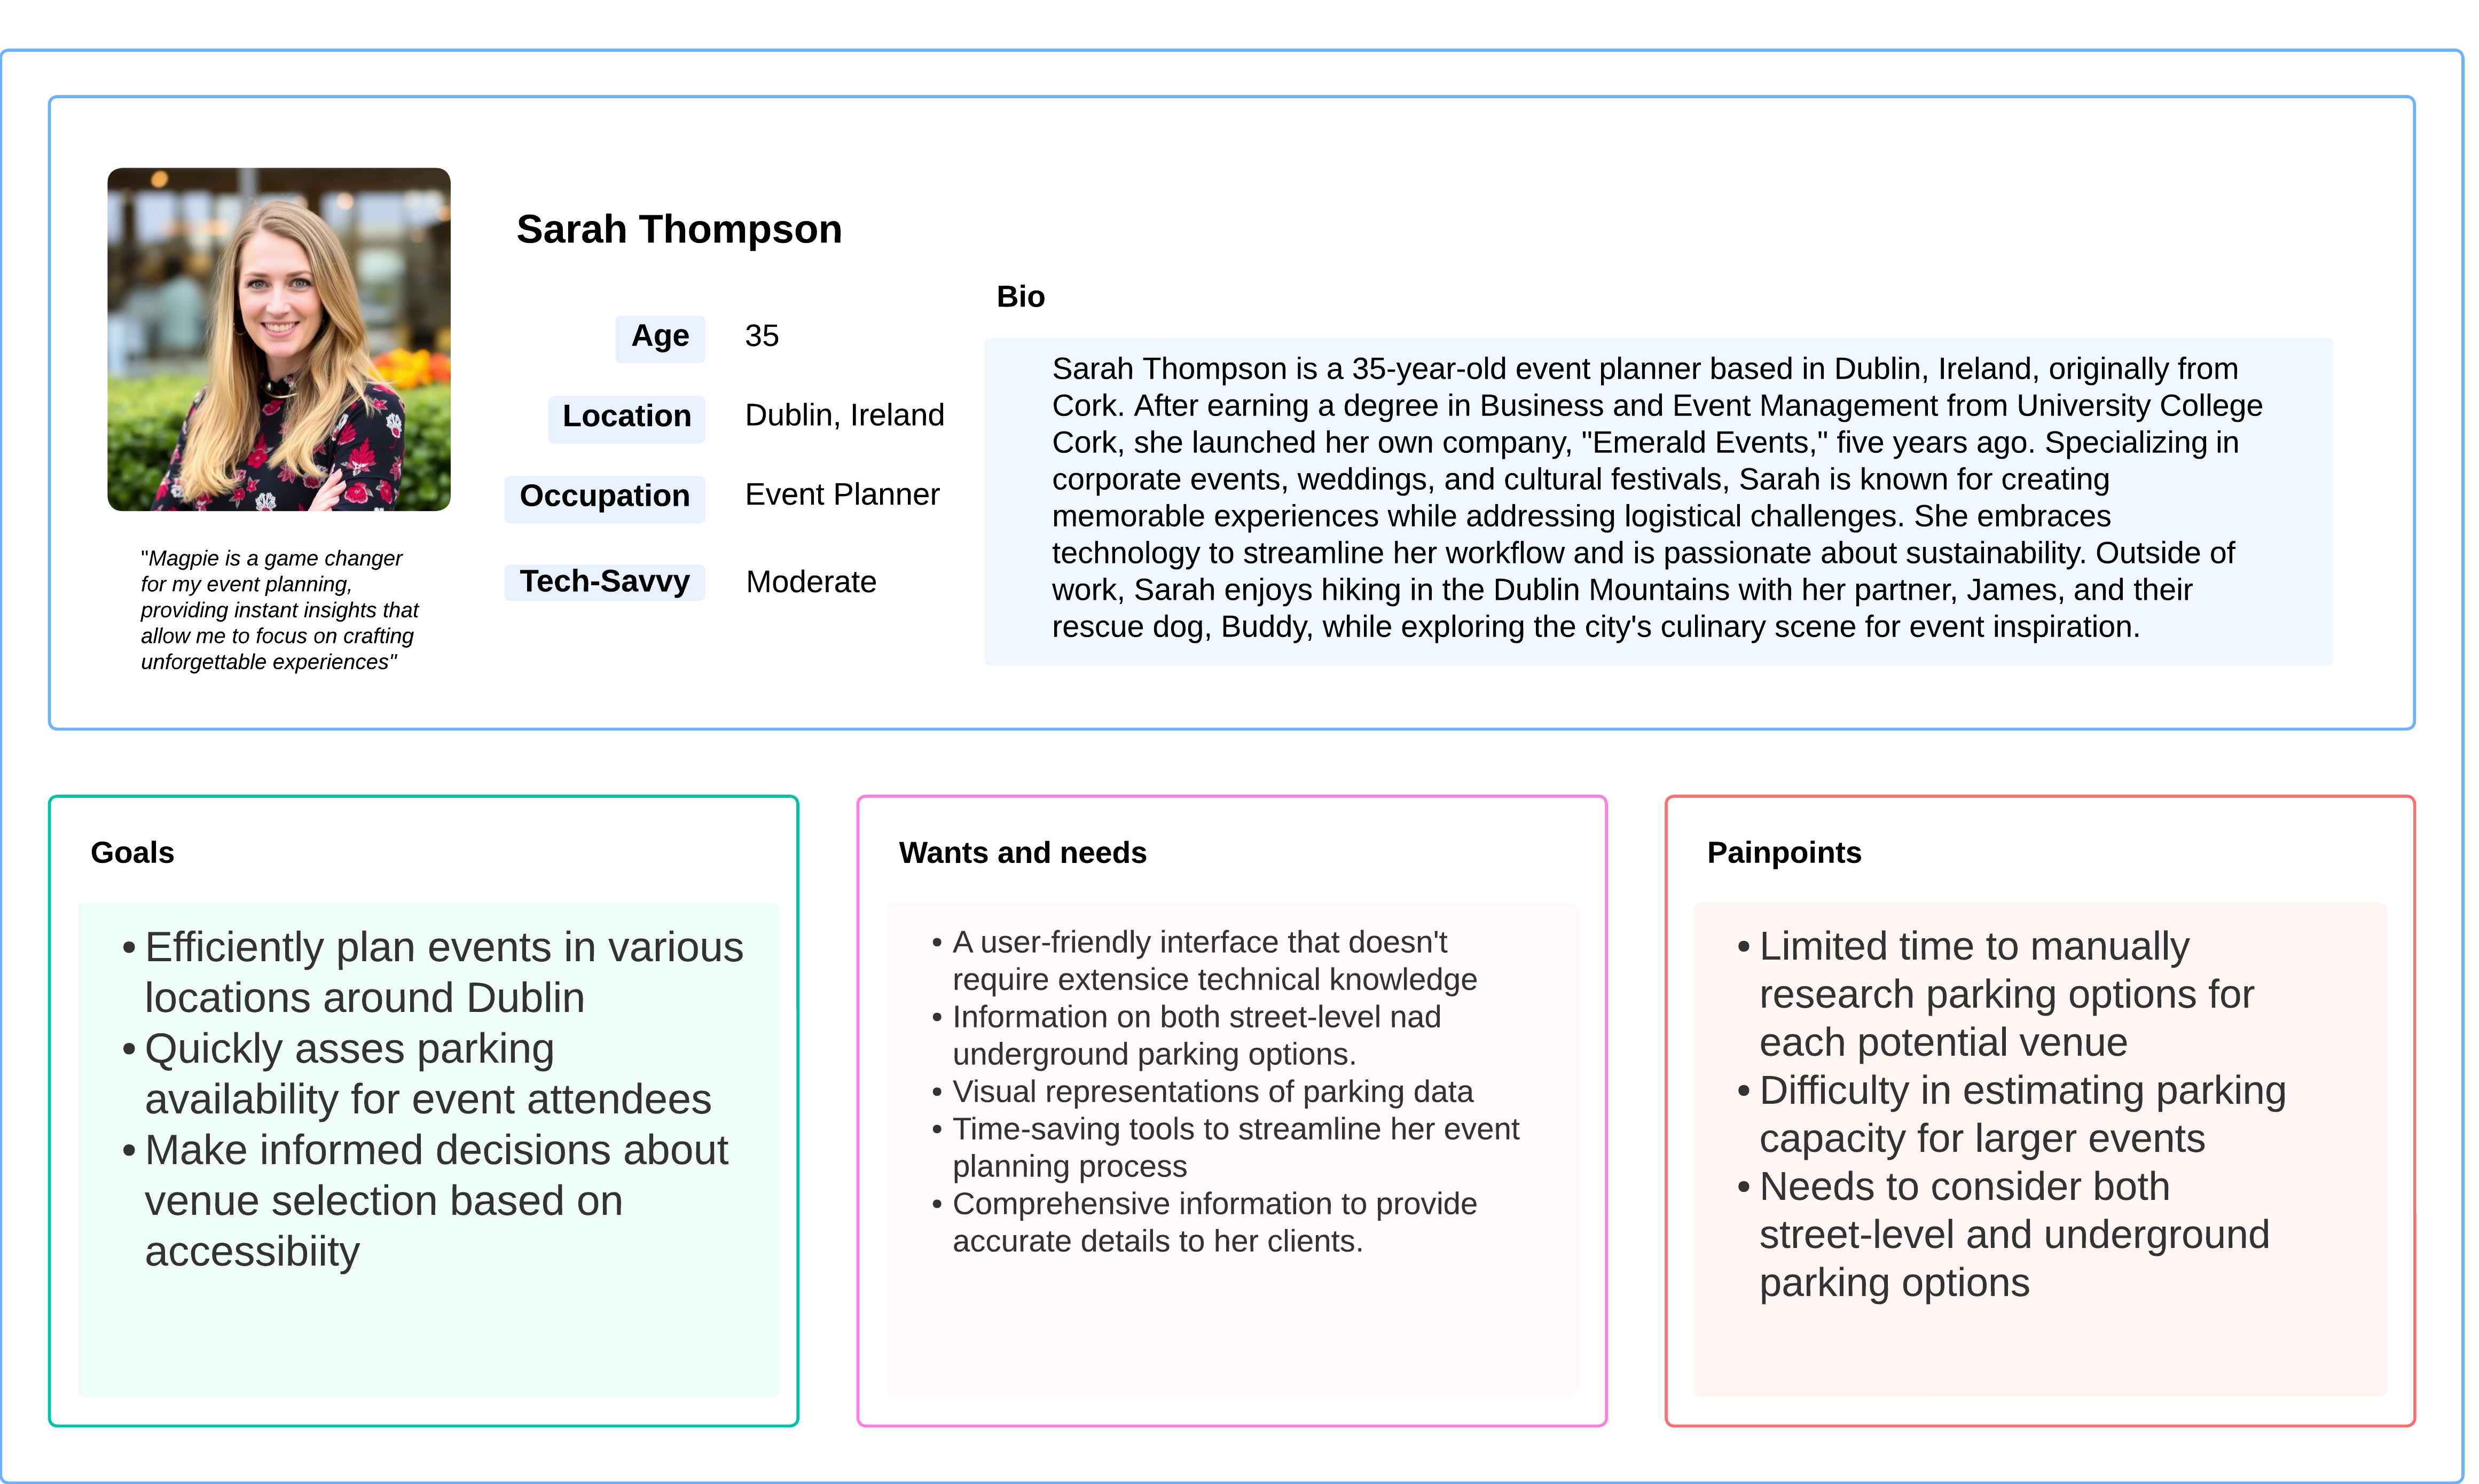
\includegraphics[width=0.8\textwidth]{images/sarah-thompson-userpersona.png}
    \caption{User persona - Sarah Thompson}
\end{figure}

\newpage{}

Currently, she faces many challenges planning events within Dublin city. She has
limited time to manually research transport and parking options and to visually
assess the accessibility of a possible venue. She's looking for a tool that will
give her a visual overview of transportation and parking options in an area,
with additional information on their location  \& their quantity. She also needs
something quick and easy to use.

\subsection{Why are they important?}
Urban Planners are crucial for the holistic development of cities and towns.
(\cite{jha2021review})They ensure that urban development is sustainable,
balancing economic growth and environmental protection. (\cite{lei2021urban})
Urban planners guide cities towards more efficient uses of land, better
transport systems, and overall increasing the quality of life of residents.
(\cite{janpavle2022importance})

By planning for current and future needs, Urban Planners help mitigate urban
challenges such as congestion, pollution, and lack of infrastructure. Their role
is essential for ensuring that urban areas can meet the demands of growing
populations, while maintaining standard of living and environmental
sustainability.

\subsection{What problem are we solving?}
Urban Planners often face challenges with accessing and analysing data. Data is
typically siloed, making it difficult to access and analyse.
(\cite{duivenvoorden2021managing})

We aim to provide Urban Planners with a tool that allows them to access this
information in a single, easy to use, platform. This will allow Urban Planners
to streamline the initial phases of their work, decreasing the time spent on
data collection and increasing the time spent on analysis and decision making.

\subsection{Market analysis}
The identification of our target user was made possible through exploratory work
done at the beginning of the project timeline. A research survey was conducted
using Microsoft Forms, sent out to county councils, planners, firms and the
TUDublin mailing list, to answer key demographic \& product questions:
\begin{enumerate}
    \item{Who is our primary target user?}
    \item{What kind of amenity data do they access and how?}
    \item{What devices/tools do they primarily use?}
    \item{Are they satisfied with those tools?}
    \item{Would they consider Magpie useful in filling the gaps in their toolset?}
\end{enumerate}

\newpage{}

\subsubsection{Demographic data}
This first section of the survey covered demographic data, to allow us to build a profile for the respondents. Personal identifiable information was not collected for the purposes of anonymity.

We had a total of 118 respondents, which we divided into 2 categories:

\emph{User A}: Respondents who did not use amenity data in their work = \textbf{88 users}.
\emph{User B}: Respondents who used amenity data in their work = \textbf{30 users}.
Splitting the respondents allows us to better analyse the answers in the context of if they belong to our primary or our secondary target user group.

Both user groups were evenly distributed in employment sector and counties they work in, as illustrated in the figures below.

%user sector distribution
\begin{figure}[htbp]
    \centering{}{}
    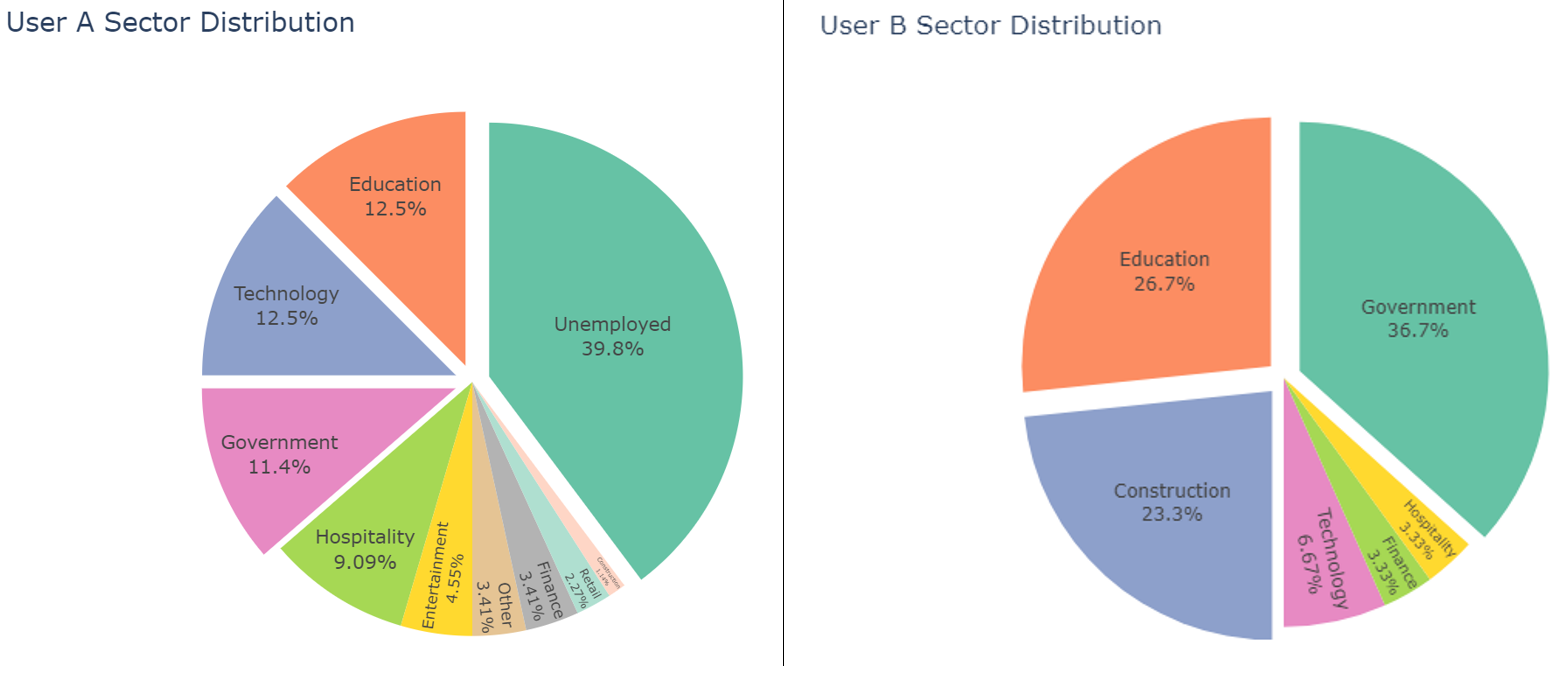
\includegraphics[width=0.8\textwidth]{images/mr-sector-distribution.png}
    \caption{Market analysis - User Sector Distribution}
\end{figure}

%user sector distribution
\begin{figure}[htbp]
    \centering{}{}
    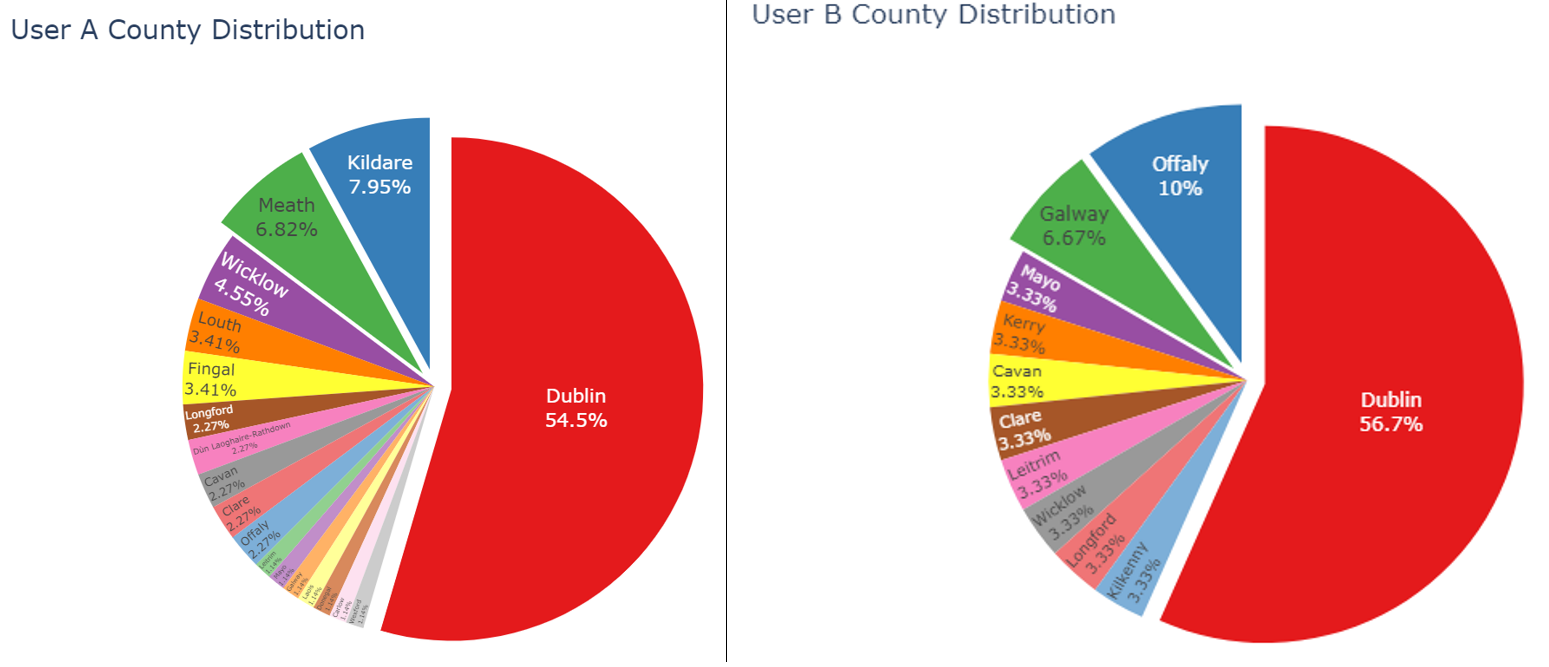
\includegraphics[width=0.8\textwidth]{images/mr-county-distribution.png}
    \caption{Market analysis - User County Distribution}
\end{figure}

\newpage{}

\subsubsection{Amenity data}
This section specifically questions respondents in the User B group on their use of amenity data in their work.

We can see that the most common amenity data accessed is transportation.

%amenity data type accessed
\begin{figure}[htbp]
    \centering{}{}
    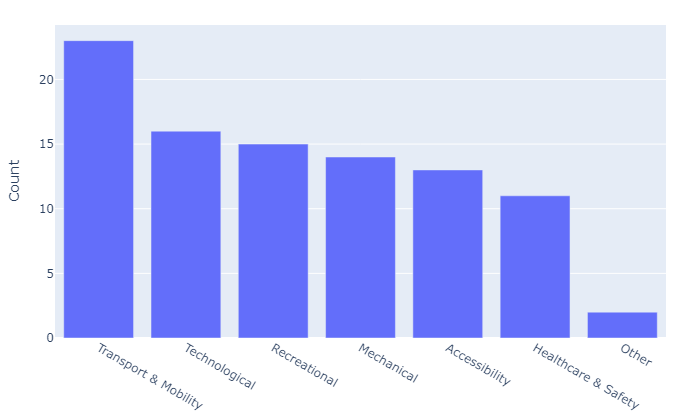
\includegraphics[width=0.8\textwidth]{images/mr-userb-amenity.png}
    \caption{Market analysis - User B Amenity Data Type Distribution}
\end{figure}

\subsubsection{Devices \& Tools}
This section looks at the devices used by both users groups, as well as the
applications or tools they are using to access amenity data.

User A was specifically questioned on which device they use for navigation and
at what frequency.

%device + freq user A
\begin{figure}[htbp]
    \centering{}{}
    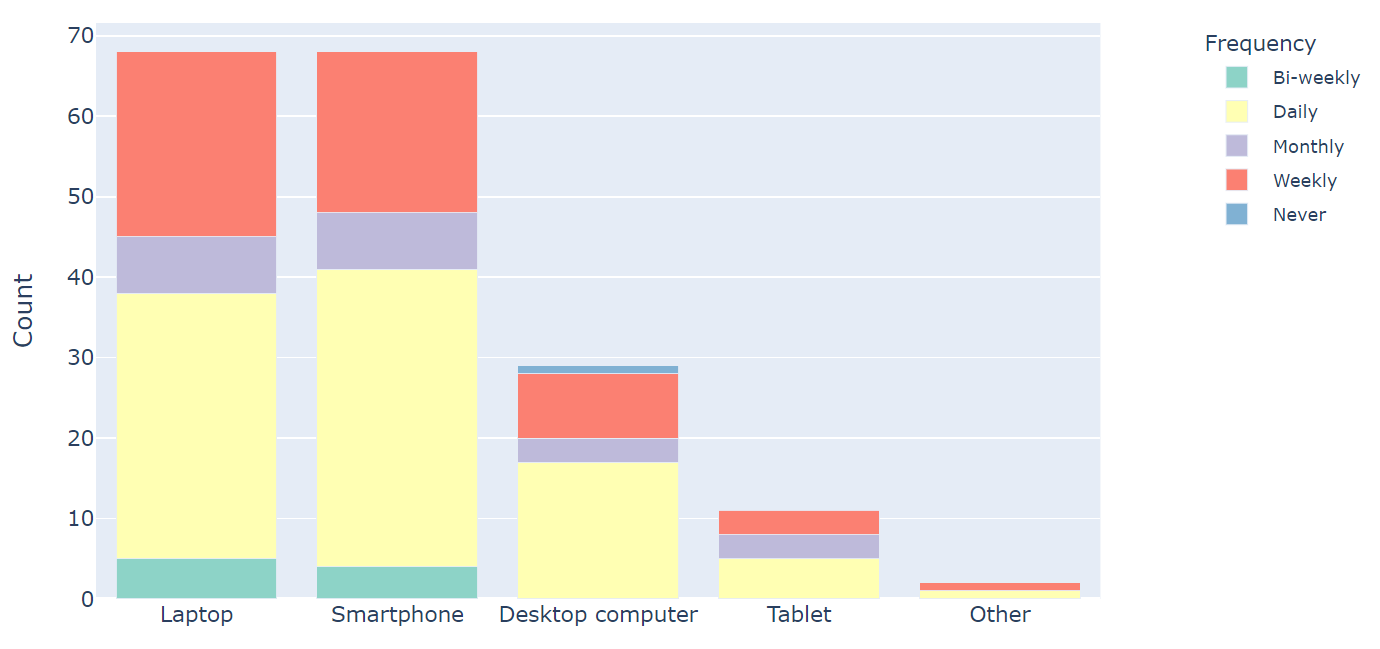
\includegraphics[width=0.8\textwidth]{images/mr-usera-device-freq.png}
    \caption{Market analysis - User A Preferred device \& Usage frequency}
\end{figure}

User B was specifically questioned on which device they use for their day-to-day
work, as well as what tool they are currently using to access amenity data.

%device + freq user B
\begin{figure}[htbp]
    \centering{}
    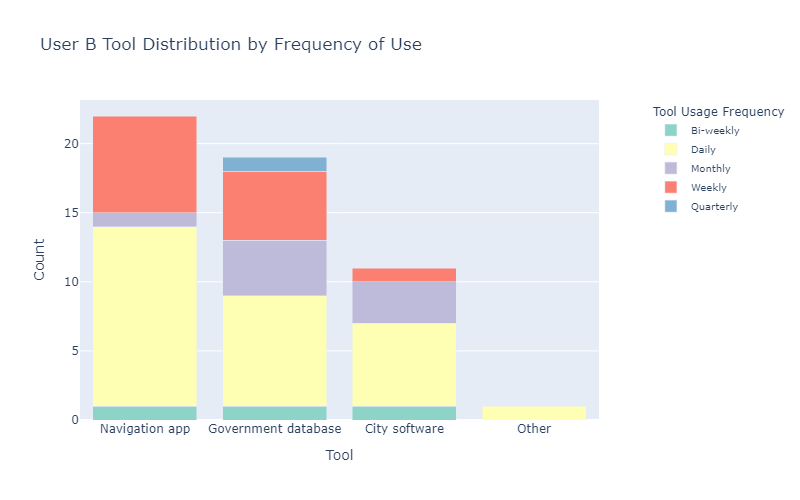
\includegraphics[width=0.8\textwidth]{images/mr-userb-tool-freq.png}
    \caption{Market analysis - User B Tool type \& Usage frequency}
\end{figure}

User B were also questioned on their satisfaction with their current tool. More
than 50\% of respondents said they weren't completely satisfied, citing
incomplete information, lack of user friendliness and poor speed as reasons.

%tool + satisfaction user B
\begin{figure}[htbp]
    \centering{}
    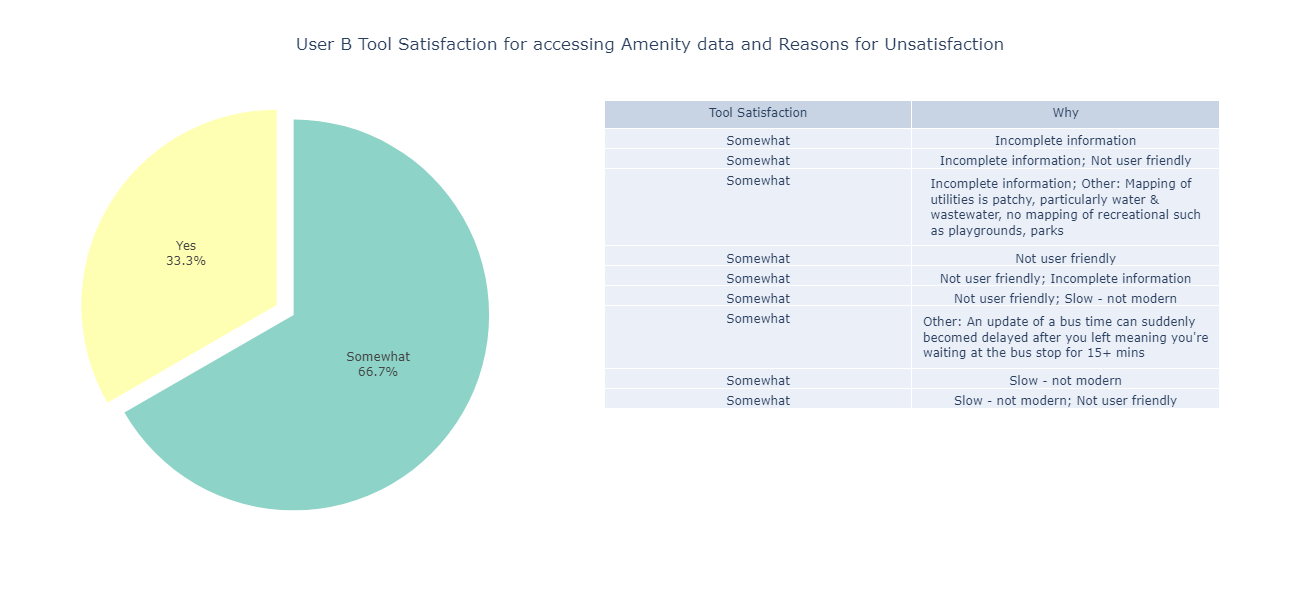
\includegraphics[width=0.8\textwidth]{images/mr-userb-tool-satisfaction.png}
    \caption{Market analysis - User B Tool satisfaction \& Usage frequency}
\end{figure}

\subsubsection{Thoughts on Magpie}
Lastly, this section covers questions regarding Magpie's potential to bridge the
gap in modern visualizing solutions.

%magpie usefulness user a
\begin{figure}[htbp]
    \centering{}
    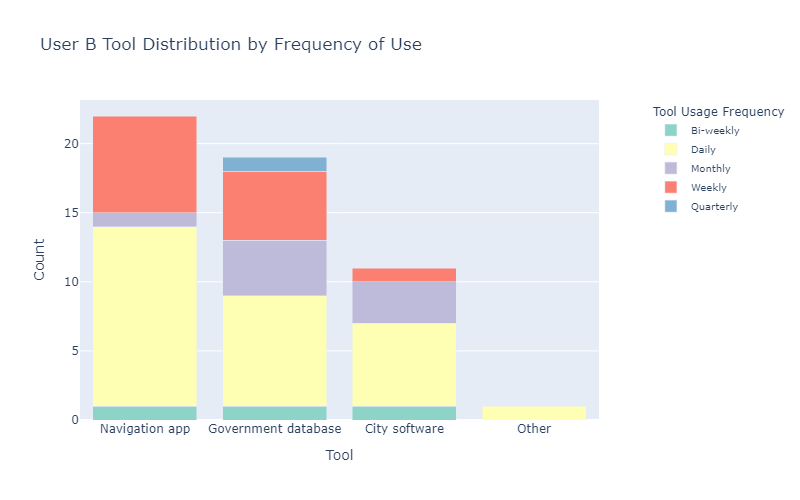
\includegraphics[width=0.8\textwidth]{images/mr-userb-tool-freq.png}
    \caption{Market analysis - User A Thoughts on Magpie}
\end{figure}

%magpie usefulness user b
\begin{figure}[htbp]
    \centering{}
    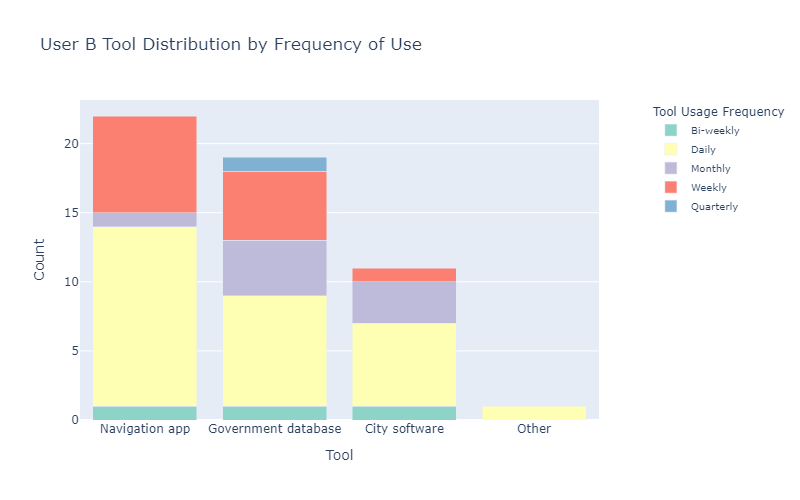
\includegraphics[width=0.8\textwidth]{images/mr-userb-tool-freq.png}
    \caption{Market analysis - User B Thoughts on Magpie}
\end{figure}

Both user groups found that Magpie would be useful to access amenity data, less
than 5\% citing it would be impractical because either they did not require
access to this information, or other tools such as Google Maps already satisfied
their needs.

Users from group B were also asked what additional features they would like to
see on Magpie. The highest rated ones were a \textbf{search functionality} and
\textbf{filters}.

%magpie usefulness user b
\begin{figure}[htbp]
    \centering{}
    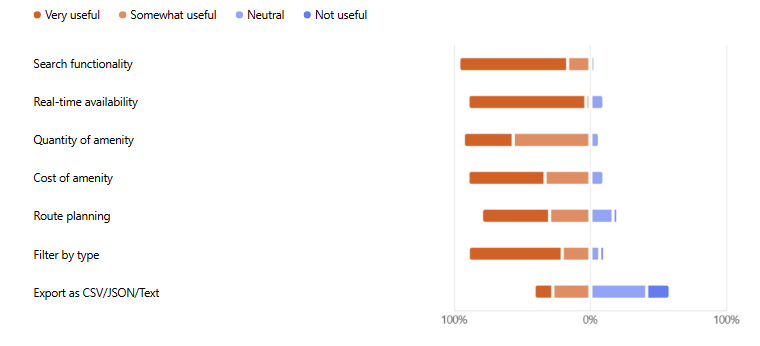
\includegraphics[width=0.8\textwidth]{images/mr-extra-features.png}
    \caption{Market analysis - User B Rating Additional Features}
\end{figure}

\textbf{Overall}, this exploratory work allows us to confirm our primary and
secondary target users as \emph{urban planners} and \emph{general users}
respectively.

Additionally, it gave us insight into a feature list to implement throughout
development, as well as competitors to research into.

\end{document}

\section{Technical Problem}
\subsection{Why does our system exist?}
In our research, we couldn't find a singular system that allows users to gain a
general overview of public amenities, for example, parking, bike infrastructure,
or public transport. In Ireland and the United Kingdom, the prevalence of proper
digitised records in county administrations varies wildly
(\cite{WebAccessibilityIreland}). Some make use of state-of-the-art geographical
information systems (GIS) while others rely on spreadsheets which are manually
kept up to date. (\cite{mcguirk2001changing})

A system that would allow users to quickly inspect a combined dataset
grounded in automatically generated, real-world data could accelerate processes
like planning permissions, urban development, or resource allocation. This
applies especially to smaller counties that may not have personnel experienced
in this area. (\cite{clark2002amenities})

Improving how governments allocates resources could lead to
improvements in efficiency, making public services more attainable, even for
smaller communities. For example, having accurate data on public transport and
bike infrastructure encourages more people to choose sustainable modes of
transport, helping reduce carbon and noise emissions (\cite{MUGION20181566}). It
could also make it easier for people in underserved communities to access
important services, such as housing, thus helping to bridge social gaps.
(\cite{allen2015understanding})

\newpage{}

Currently, solutions are fragmented, focusing on just one type of
amenity, like transport or housing, without giving a full picture. Even the more
advanced GIS systems, while powerful, usually need a lot of manual input or
additional programming, which smaller municipalities or organizations might not
be able to handle. For example, to find parking spots in an area, the user needs to
either bring their own dataset or they have to perform computer vision analysis
themselves. While \textit{ArcGIS} includes tools to run deep learning on raster
images, the process is far from straight forward. Many of these GIS tools are also
expensive, or require specialised training, making them out of reach for smaller
boroughs or counties. (\cite{kaufmann2022scaling})

\subsection{The core technical problem}
The problem at the heart of our project is to find a way to collate and
visualize useful data about public amenities, without the need for any existing
information or manual data entry. This would allow the solution to be useful, no
matter the state of the users digital records. Relying purely on existing data
would do nothing to reduce the divide between counties with more data and
counties with less data. This necessitates the creation of an interconnected
series of modules that form a pipeline, for the automatic extraction and fusion
of data.

In order to present users with a map containing information about the
number of public amenities, we must first identify them. Our biggest technical
challenge is the extraction of these data points. Different forms of public
amenities exist in satellite imagery, we can combine this with other data
sources, interweaving them, and producing a better result.

Detecting public amenities from overhead views is a non-trivial process,
as satellite imagery suffers from low resolution, occlusion, seasonal changes, or
cloud cover. This means classifying specific objects can be complicated, and can
take a lot of time and processing power. For instance, the task of quantifying
on-street parking is dependent on reliably detecting cars that are not actively
participating in traffic (in aerial images). Not only that, but the detected
points in the images must be mapped back onto real-world coordinates to be of
any utility.

Ensuring consistency between the extracted data, and other data sets,
can have its own pitfalls. For example, compensating for:

\vspace{-3mm}
\begin{itemize}
  \item{different precision in geographical alignment}
  \item{varied update frequencies}
  \item{different data formats}
\end{itemize}
\vspace{-3mm}

Not only can data be geographically misaligned, but since satellite
data is only a snapshot in time, it can lead to temporal misalignment as well.
Even the appearance of amenities can change depending on their location. While
cars look more or less the same anywhere on Earth, the same cannot be said for
public transport links, housing or hospitals, which could lead to difficulties
achieving the same level of accuracy in different regions. Processing a large
amount of data like can be difficult and finding a strategy to do this
efficiently is necessary.

\newpage{}

\subsection{A review of similar systems}

\textbf{Parkopedia}

\begin{figure}[htbp]
  \centering
  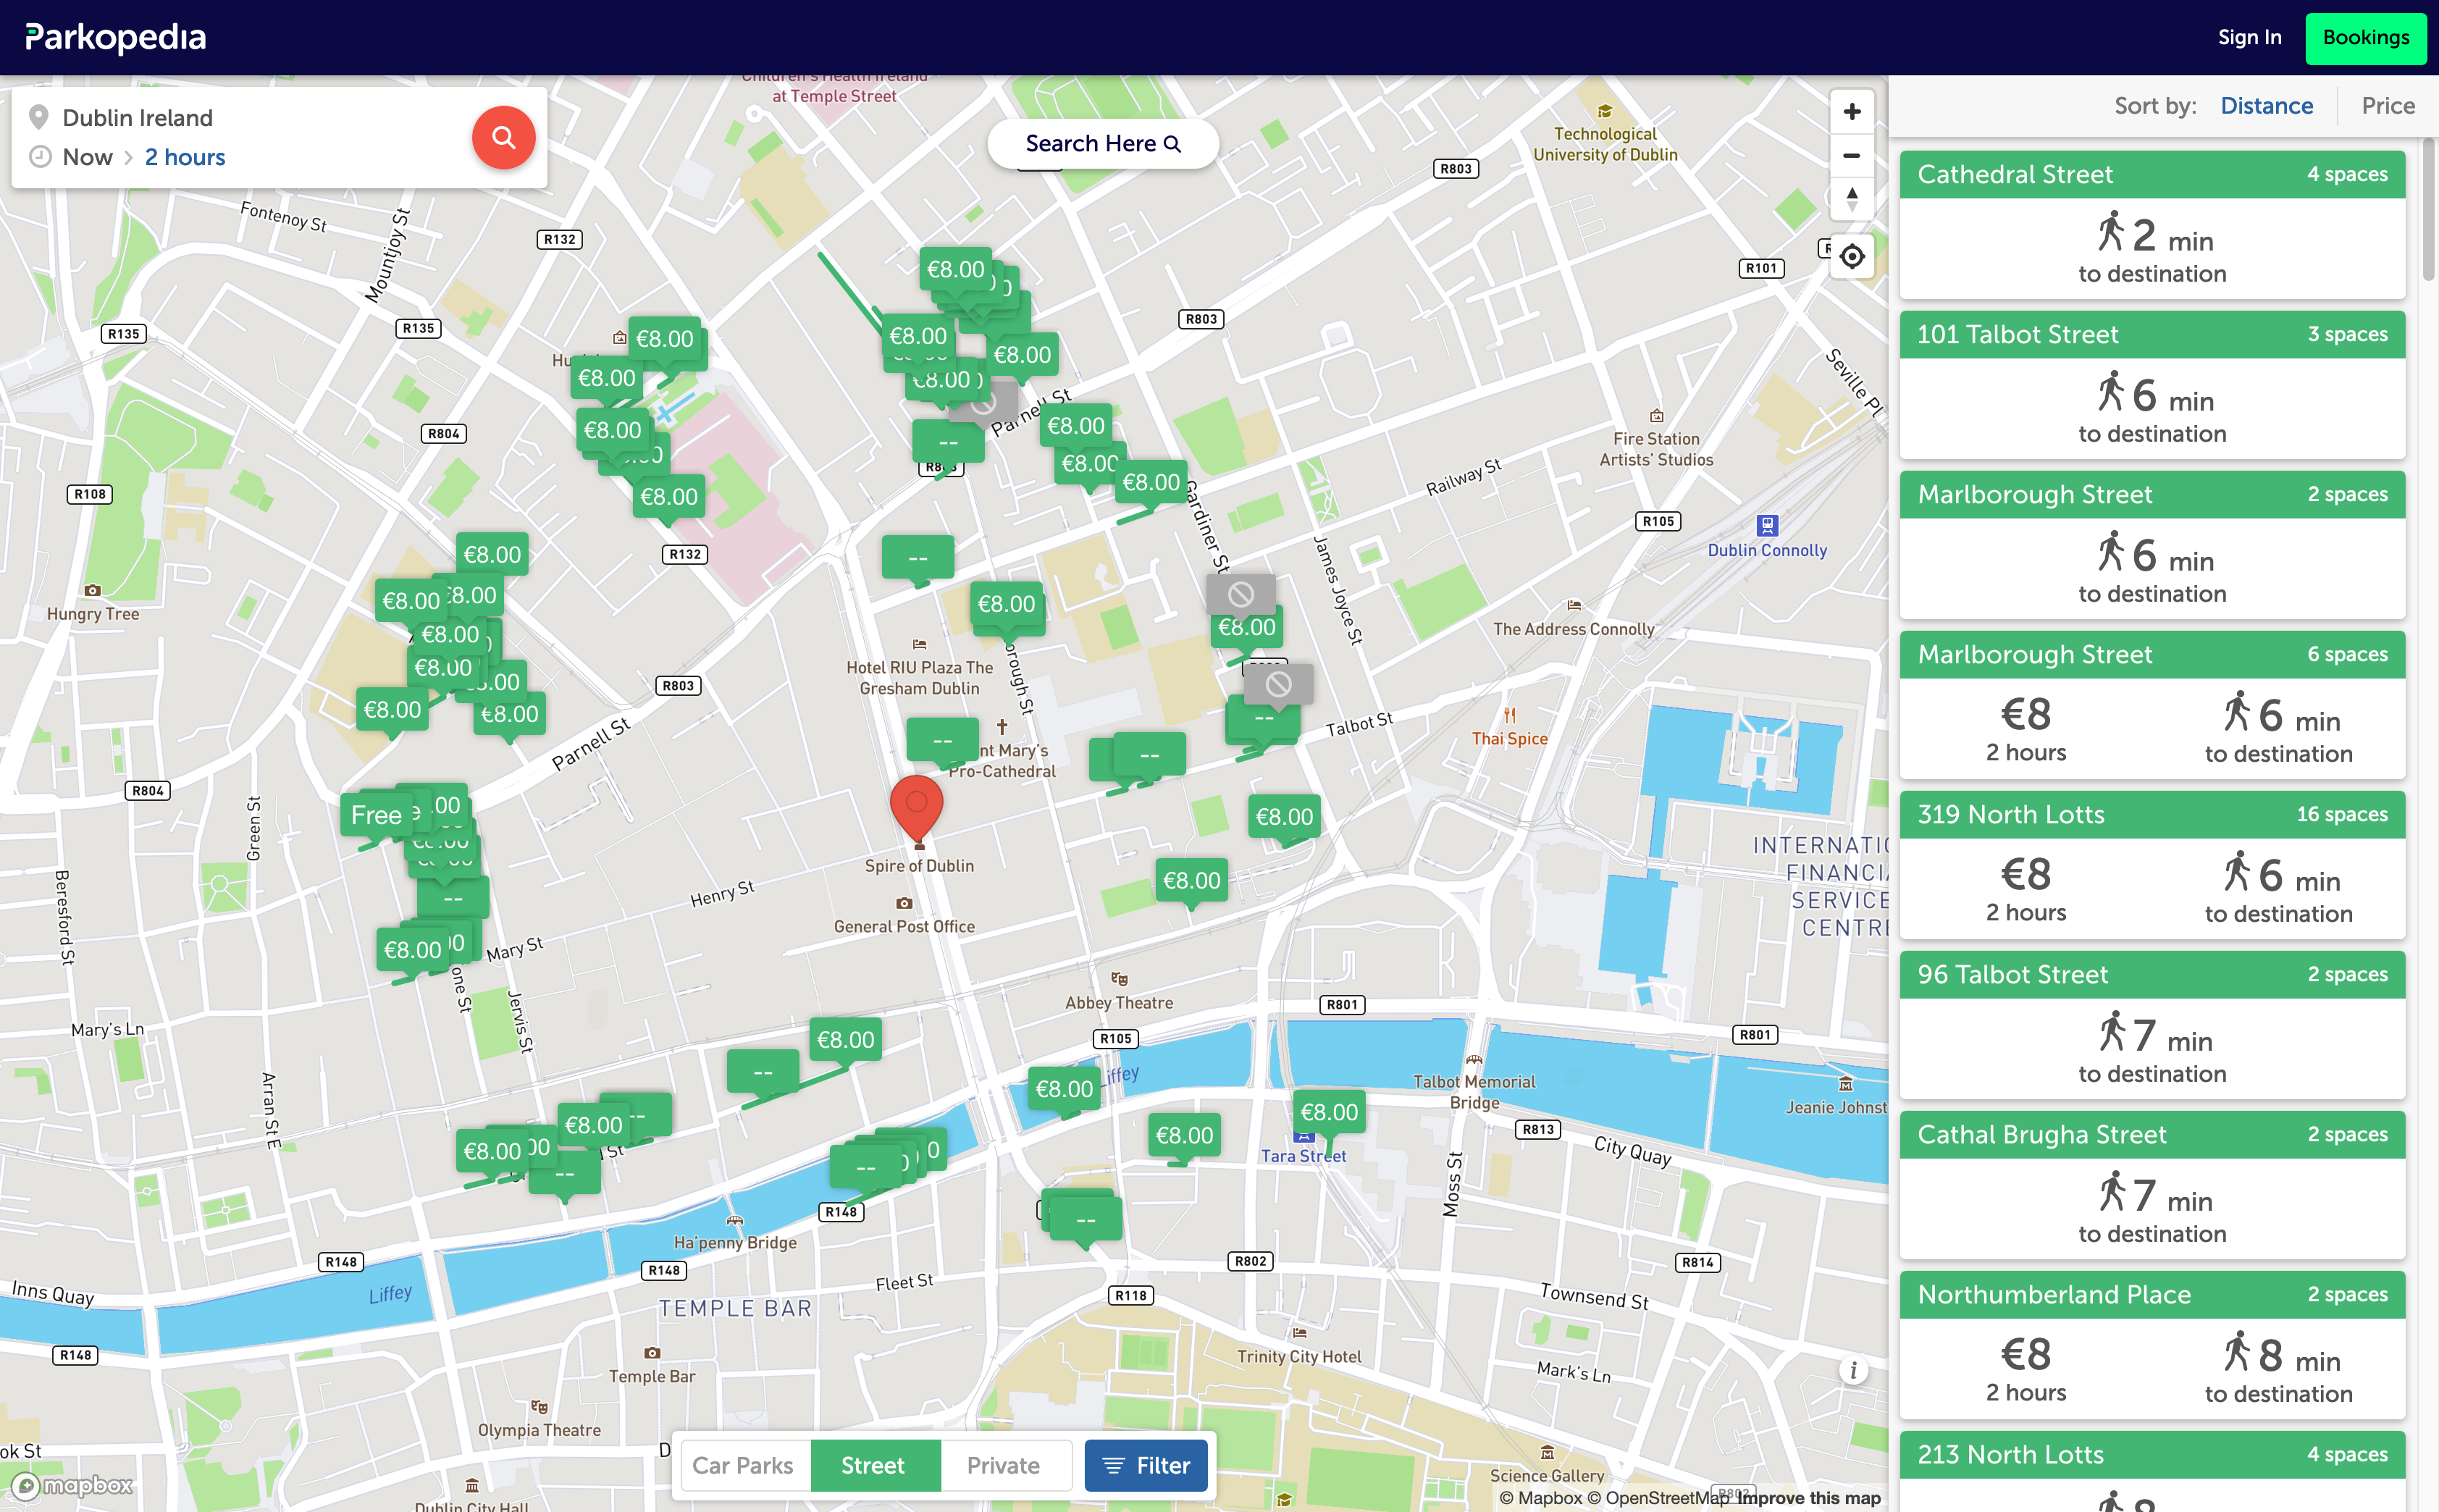
\includegraphics[width=\columnwidth]{images/parkopedia.png}
  \caption{Example of parkopedia}
  \label{fig:parkopedia}
\end{figure}

\textit{Parkopedia}\footnote{https://www.parkopedia.com/} is a web
application that allows users to find parking in many cities around the world.
They offer location and pricing data on parking garages, on-street parking and
parking on private property.

It is similar to \textit{Magpie} in the sense that it allows users to
gain a quick overview of all parking options in their area.

Our system differentiates itself from \textit{Parkopedia} in three
main ways:
\vspace{-3mm}
\begin{itemize}
  \item{\textbf{Data fusion:} Our system integrates data from publicly available
  sources, combining multiple datasets to provide a more comprehensive overview
  of public amenities -- not just parking.}
  \vspace{1.25mm}

  \item{\textbf{Aggregated data:} Our system offers a high-level overview of the
  amount of available amenities in a certain radius. This would be possible with
  the data from \textit{Parkopedia}, but the user would have to manually
  retrieve the data in which they are interested in analysing.}
  \vspace{1.25mm}

  \item{\textbf{No reliance on manual data entry:} Unlike
  \nobreak{\textit{Parkopedia}}, which relies on user-submitted information, we
  automatically acquire and fuse datasets. This pipeline allows us to keep
  information up-to-date and adapt our system to new regions without the need
  for manual data input.}
  \vspace{1.25mm}

\end{itemize}

\newpage{}

\textbf{ArcGIS}

\begin{figure}[htbp]
  \centering{}
  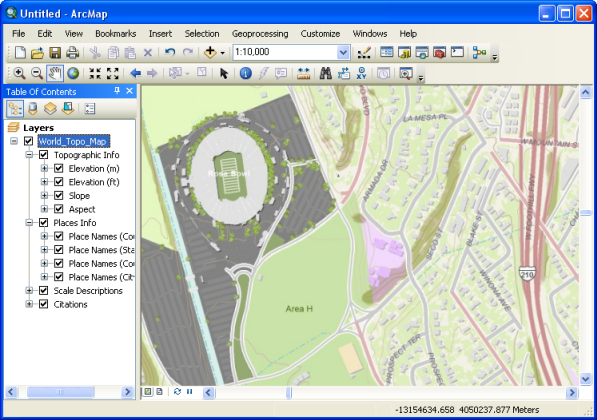
\includegraphics[width=0.85\columnwidth]{images/arcgis.png}
  \caption{Example of ArcGIS}
  \label{fig:arcgis}
\end{figure}

Systems like \textit{ArcGIS}\footnote{https://www.arcgis.com/} target
mainly expert users like cartographers and researchers. These systems are powerful
and feature-rich tools for professionals. While \textit{ArcGIS} is able to produce
the same overview offered by our system, it is different in these key aspects:

\begin{samepage}
\begin{itemize}
    \item{\textbf{Ease of use:} The goal of our system is to cater to a broad
    range of users, not just experts. Systems like \textit{ArcGIS} require
    specialised domain knowledge, as it's aimed at professional users. While
    \textit{ArcGIS} offers powerful tools, it can be overwhelming for the more
    Non-Expert User who needs a quick overview of public amenities without engaging
    with advanced features.}
  \vspace{1.25mm}

  \item{\textbf{Accessibility:} GISs are a robust tool, but its access is often
  restricted lack of technical expertise. Compared to \textit{ArcGIS}, our
  system is less versatile. However, our system is more streamlined to offer- at
  a glance- an easily accessible way of gauging information about public
  amenities. This makes sure that users from all backgrounds can utilize our
  system without the need for specialised training.}
  \vspace{1.25mm}

\end{itemize}
\end{samepage}

\newpage{}

\subsection{Conclusion}

The need for a system like ours arises from the fragmented state of public
amenity data and the barriers to accessing it efficiently. By addressing these
challenges, our system offers a combination of automated data extraction,
fusion, and visualization that caters to users across technical skill levels.
Unlike existing solutions, which are either too specialized or demand
significant expertise and resources, our system prioritizes inclusivity and
accessibility.

Through the integration of real-world data we aim to bridge gaps in resource
allocation, improve efficiency in urban planning, and support sustainable
development. By lowering the entry barriers for smaller municipalities and
underserved regions, the system democratizes access to critical geographical
insights and also contributes to fostering equitable and sustainable
communities.

This project lays the groundwork for a more informed approach to public planning
and resource distribution, with the potential to evolve into a versatile tool
that supports diverse stakeholders in addressing the complexities of modern
urban and regional development.

\newpage{}

\section{Technical Solution}
\documentclass[preview]{standalone}
\begin{document}

\subsection{System Overview}
\begin{figure}[htbp]
    \centering{}
    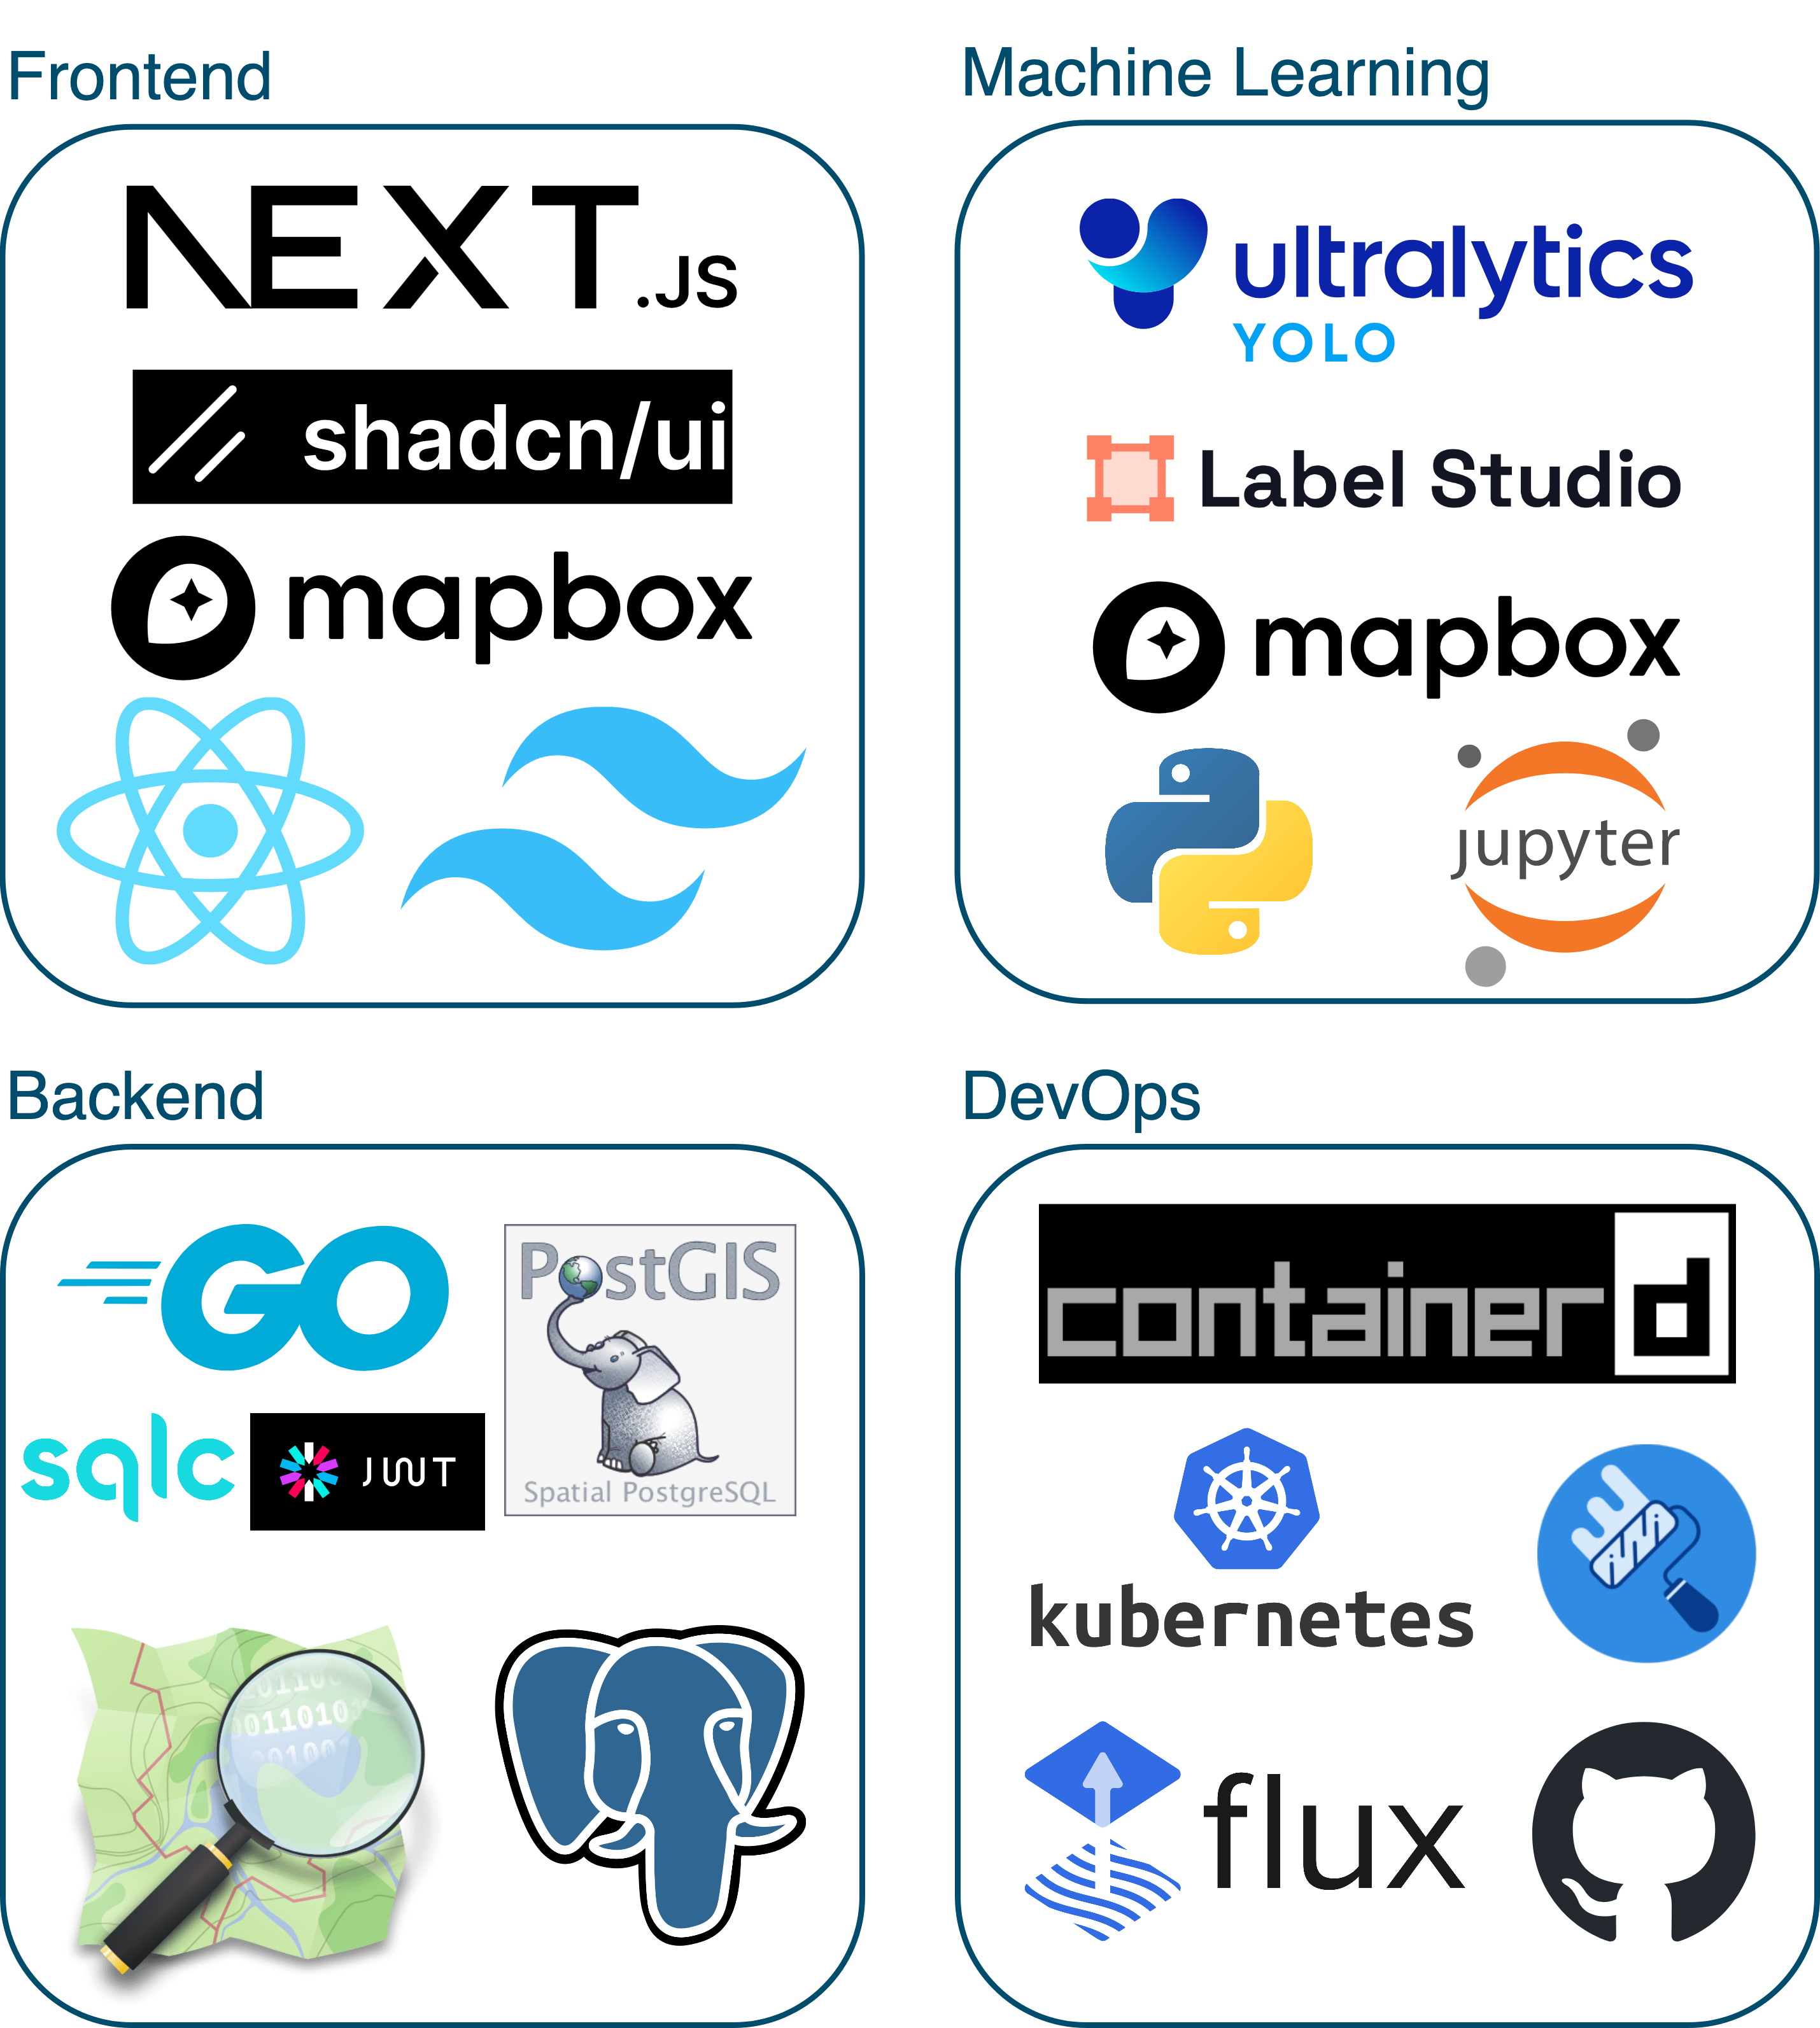
\includegraphics[width=0.5\textwidth]{images/stack_grid.png}
    \caption{Magpie's technology Stack}
\end{figure}

\subsubsection{Frontend Technologies}

The frontend stack plays a critical role in providing a smooth and interactive user experience for the application. It is built on top of modern web technologies, each serving a unique purpose:

\begin{itemize}
    \item{} \textbf{Next.js:} This React framework offers server{-}side rendering (SSR) and static site generation (SSG), which improve performance, SEO, and user experience.
    \item{} \textbf{React:} As the foundation of the frontend, React allows for component{-}based development, making the interface scalable and easy to maintain.
    \item{} \textbf{TailwindCSS:} A utility{-}first CSS framework that simplifies styling by providing ready{-}to{-}use classes, enabling rapid UI development.
    \item{} \textbf{shadcn/ui:} A collection of reusable UI components that work seamlessly with Next.js and React, enhancing productivity and consistency across the application.
    \item{} \textbf{Mapbox:} A powerful mapping platform that enables interactive, customizable maps. It helps visualize geospatial data effectively, which is key for location{-}based services in this project.
\end{itemize}

These technologies combine to create an engaging user interface that is both functional and visually appealing, allowing users to interact with location{-}based data and services efficiently.

\subsubsection{Machine Learning Technologies}

The machine learning stack adds intelligent capabilities to the system, enabling advanced features such as object detection. Here’s a breakdown of the tools in this section: 

\begin{itemize}
    \item{} \textbf{Ultralytics YOLO:}  An object detection model that helps identify specific objects in images, enhancing the system's ability to recognize and interpret visual data. 
    \item{} \textbf{Label Studio:} A flexible tool for annotating datasets, enabling easy labeling of images, text, and audio. This is crucial for creating high-quality datasets to train machine learning models like YOLO. 
    \item{} \textbf{Python:} The primary language for developing our scripts and running machine learning models, Python supports image processing, model training, and analysis. 
    \item{} \textbf{Jupyter Notebooks:} An interactive platform that allows data scientists to experiment with code, visualize results, and document their machine learning processes. 
\end{itemize}

These technologies allow the application to process and analyse data intelligently, enabling features such as object recognition in geographical data and personalized insights.

\subsubsection{Backend Technologies}

The backend stack ensures the application can handle large volumes of data, manage user requests, and perform complex computations. Some of the key technologies include:

\begin{itemize}
    \item{} \textbf{Go (Golang):} A highly performant programming language ideal for building scalable backend services.
    \item{} \textbf{PostGIS:}  An extension of \textbf{PostgreSQL}, PostGIS adds geographic object support to the database, making it easier to work with spatial data like maps, coordinates, and distance calculations.
    \item{} \textbf{sqlc:} A SQL code generator that helps developers write type{-}safe database queries in Go, reducing the chances of errors during database interactions.
    \item{} \textbf{JWT:} A compact, URL{-}safe token format used for securely transmitting information between parties, often for authentication and authorization purposes.
\end{itemize}

By leveraging these tools, the backend is capable of managing complex spatial data, performing queries on geospatial data, and ensuring smooth user interactions through highly responsive APIs.

\subsubsection{DevOps Technologies}

The DevOps stack ensures that the infrastructure supporting the application is reliable, scalable, and easily deployable. Key technologies in this section include:

\begin{itemize}
    \item{}  \textbf{Containerd:} A core container runtime that manages containerized applications, ensuring consistency across different environments (development, staging, production).
    \item{} \textbf{Kubernetes:} An orchestration platform for automating the deployment, scaling, and management of containerized applications. It allows the system to scale effortlessly based on demand and ensures high availability.
    \item{} \textbf{Flux:} A tool for continuous delivery and GitOps, Flux automates deployments by integrating with Git repositories. Changes made to the codebase are automatically reflected in the deployed infrastructure, ensuring consistency and reducing manual intervention.
    \item{} \textbf{GitHub:} The widely{-}used platform for version control and collaboration. GitHub supports seamless development workflows by enabling pull requests, code reviews, and version tracking.
\end{itemize}

Together, these tools create a robust DevOps pipeline that automates deployment, enhances reliability, and ensures that the application can handle scaling demands as it grows.

\subsubsection{Integration and Synergy}

The combination of frontend, backend, machine learning, and DevOps technologies ensures that the system functions as a seamless whole. Here's how the different parts work together:

\begin{itemize}
    \item{} The \textbf{frontend} presents an intuitive interface to users, allowing them to interact with location data, maps, and insights.
    \item{} The \textbf{backend} handles the heavy lifting, managing the spatial data, processing queries, and supporting dynamic content through APIs.
    \item{} \textbf{Machine learning} capabilities add intelligence to the system, enabling features like real{-}time object detection and personalized data analysis.
    \item{} \textbf{DevOps} practices ensure that the entire application can be deployed and scaled efficiently, with smooth continuous integration and deployment pipelines.
\end{itemize}

In conclusion, this tech stack forms a cohesive, scalable, and intelligent system. From object detection and efficient spatial data management to automated deployment pipelines, the technologies complement each other, resulting in a high{-}performance, feature{-}rich application.

\subsection{Data Sources}
Throughout project development, several datasets from various sources have been
used to fulfil Magpie's project goal. Below is an overview of Magpie's data
stack:
\begin{figure}[htbp]
    \centering
    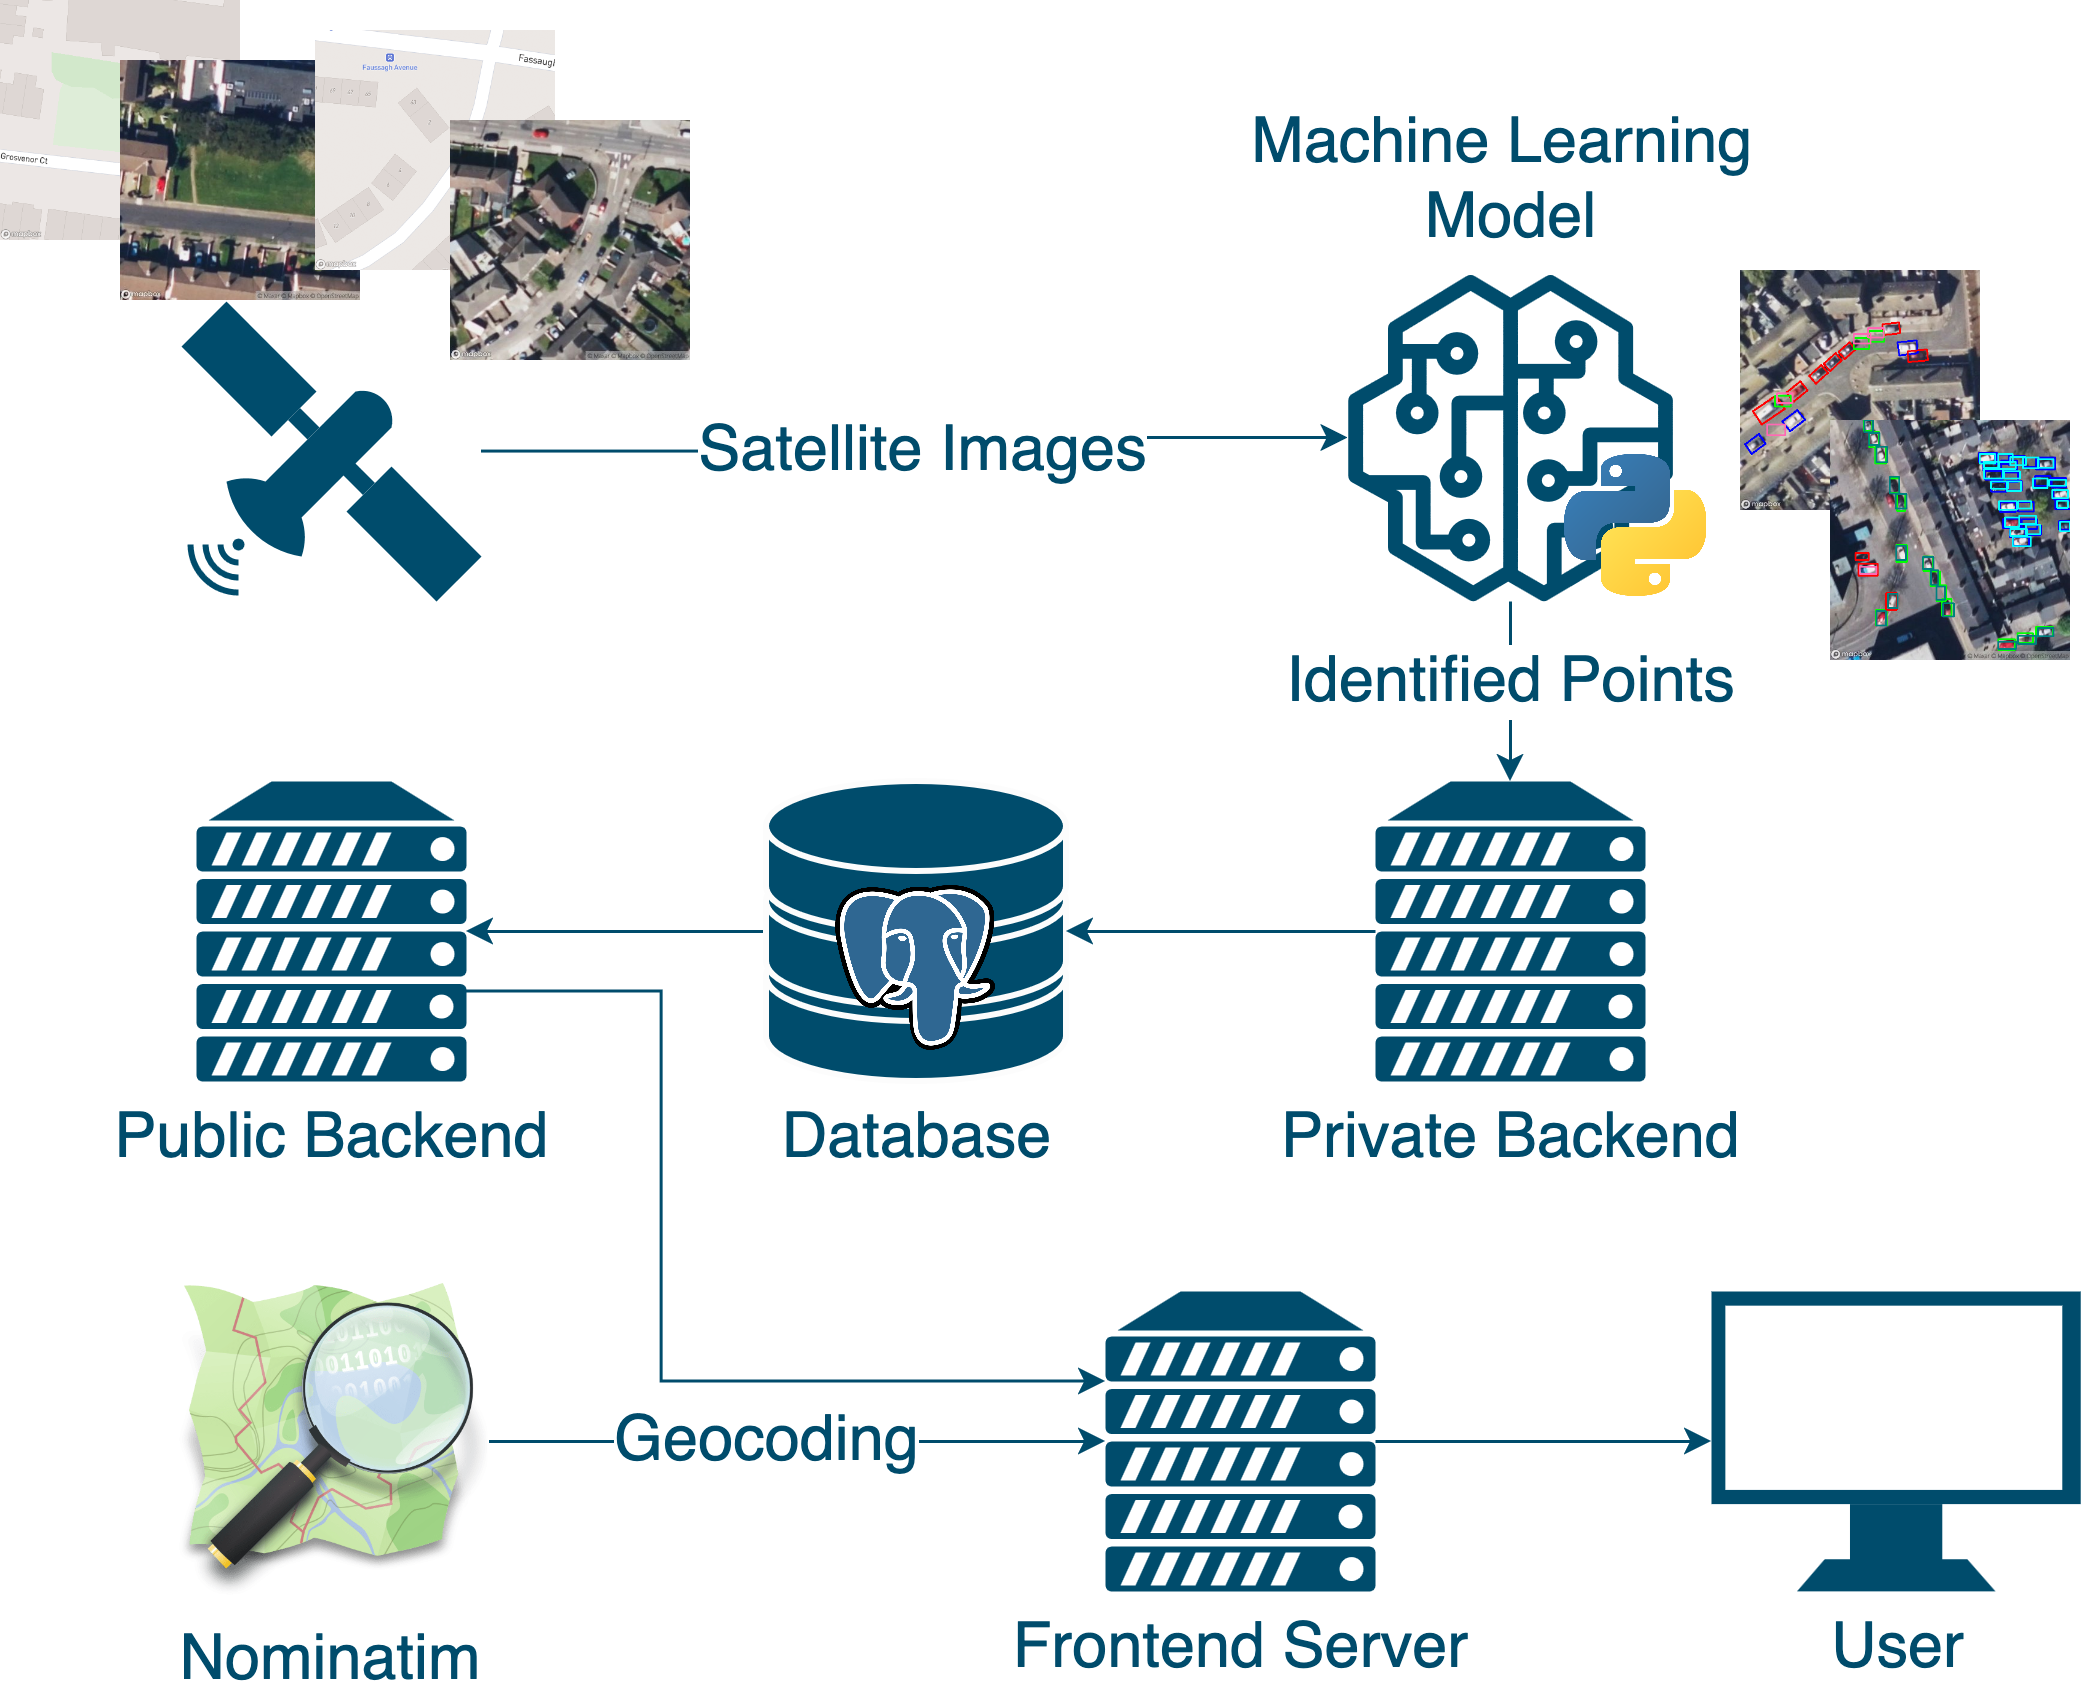
\includegraphics[width=0.7\textwidth]{images/magpie-data-stack.png}
    \caption{Magpie Data Stack}
\end{figure}

\subsubsection{Data sourcing \& Collection}
Three main categories of data have been sourced for Magpie:
\begin{enumerate}
    \item For the \emph{Machine learning models}
    \item For the \emph{Amenity data}
    \item For the \emph{Search functionality}
\end{enumerate}

\textbf{1.1 Machine learning models - Car detection}
The Mapbox Static Images API was used to retrieve all the images used for the
machine learning models of this project.

First, 250 images were downloaded using CSV data from the following sources:
\begin{itemize}
    \item \textbf{Data.gov.ie}: Online portal containing thousands of publicly
          available datasets about Ireland
    \item \textbf{Smart Dublin}: Founded by Dublin local authorities, their goal
          is to look for innovative technological solutions for local environmental,
          social, mobility, government and living issues. They also have hundreds of
          publicly available datasets
    \item \textbf{Kaggle}: a data science and machine learning platform part of
          Google Cloud where competitions are hosted, in addition to thousands of
          publicly available datasets
\end{itemize}
These CSV files contained information on the location of certain facilities such
as rentals, coach parking, public parks. This location was latitude and
longitude which we needed to input into the script to download images, as well
as the street name of that location which was used to name the downloaded image.

\begin{listing}[htbp]
    \centering
    \caption{Python script to obtain training images for ML model}
    \begin{minted}{python3}
# CSV file containing location information
df = pd.read_csv("2020-coach-parking-dcc-1.csv")
location_data = df.to_dict('records')

# function to download image using location information from CSV dataset
def get_images(name, latitude, longitude):
    url = f'''https://api.mapbox.com/styles/v1/mapbox/satellite-v9/
            static/{longitude},{latitude},18,0,0/400x400'''
    response = requests.get(url)
    print(response)
    if response.status_code == 200:
        img = Image.open(BytesIO(response.content))
        if not os.path.exists('output'):
            os.makedirs('output')

        output_folder = 'output'
        output_path = os.path.join(output_folder, f'{name}_coach_parking.png')
        img.save(output_path)
        print(f"Image saved to {output_path}")

# function to extract location & name location from CSV dataset
for place in location_data:
name = place["Street Name"]
if ("/" in name):
    name = name.replace("/", "-")
latitude = place["Latitude"]
longitude = place["Longitude"]
get_images(name, latitude, longitude)
    \end{minted}
\end{listing}

\newpage{}

Following successful model training and tuning, a further 19,536 satellite
images were downloaded spanning Dublin City area illustrated in the figure
below. The machine learning model was then applied to those images to detect the
cars.

\begin{figure}[htbp]
    \centering
    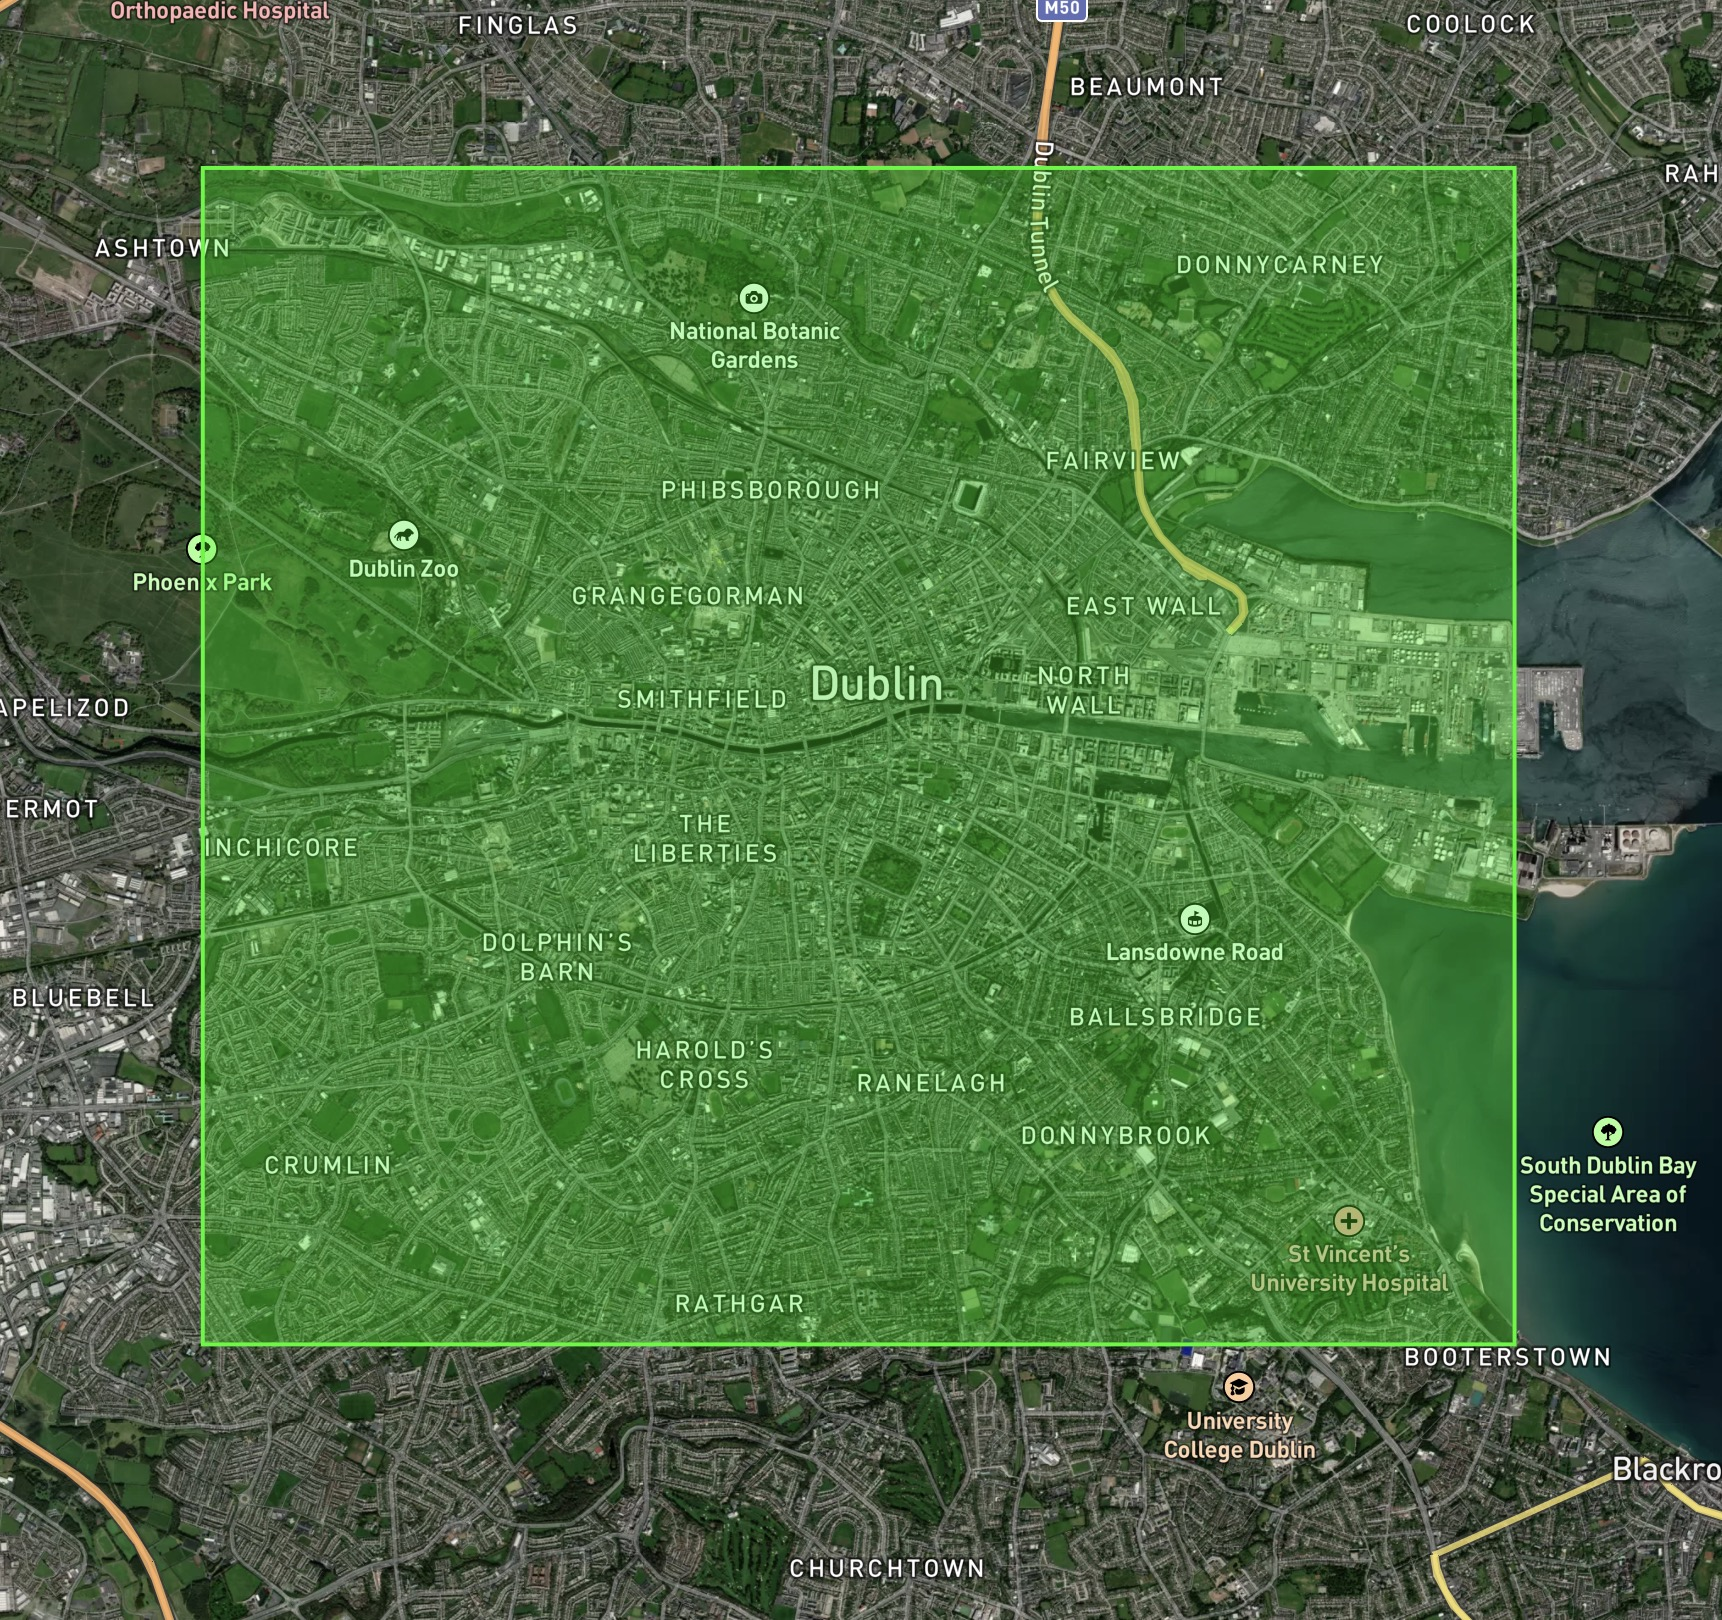
\includegraphics[width=0.6\textwidth]{images/dublin-img-area.jpg}
    \caption{Dublin Area Delimitation for Parking data}
\end{figure}

\textbf{1.2 Machine learning models - Parking detection} \\
An additional 19,536 map-view images corresponding to the satellite images used
for car detection were downloaded using the MapBox API to create the custom mask
used for detecting parked cars. Our project has two main Python scripts,
\texttt{parking\_detection.py} and \texttt{parking\_detection\_local.py} to
localize parking spots. In \texttt{parking\_detection.py}, the satellite images
(Mapbox Satellite) and corresponding road mask images (Mapbox Streets) are
retrieved for a specific area contained within a bounding box, defined by its
top-left and bottom-right coordinates, directly from the Mapbox API. From the
coordinates of the specific bounding box, the center coordinates of all the
images necessary to make up that area are calculated, and the images are then
retrieved. While in \texttt{parking\_detection\_local.py}, the original parking
detection script is adapted to run on a database of locally stored Mapbox
Satellite images and the corresponding Mapbox Streets images, covering the
entirety of Dublin city.

Extensive testing was done at all the different stages of development of the
scripts to identify the optimal thresholds and parameters using test images from
Mapbox, in a variety of scenarios including edge cases or cases prone to causing
issues.

\newpage{}

\textbf{2. Amenity data}
CSV files were collected from multiple sources mentioned above, notable
Data.gov.ie and Smart Dublin. Below is a list relative to each amenity currently
present on Magpie:
\begin{itemize}
    \item Parking meter = Data.gov.ie (link to appendix)
    \item Bike stand = Data.gov.ie (link to appendix)
    \item Public Wifi = Smart Dublin (link to appendix)
    \item Library = Smart Dublin (link to appendix)
    \item Multi-storey Car park = Data.gov.ie (link to appendix)
    \item Drinking water fountain = Data.gov.ie (link to appendix)
    \item Public toilet = Data.gov.ie (link to appendix)
    \item Bike sharing station = Data.gov.ie (link to appendix)
    \item Car parking = Novel ML technique
    \item Accessible parking = Data.gov.ie (link to appendix)
    \item Public bins = Smart Dublin (link to appendix)
    \item Coach parking = Data.gov.ie (link to appendix)
\end{itemize}
Some data cleaning and processing had to be done to obtain a new csv file with
longitudes and latitudes in the right format to send to the backend using our
send points script.

For example in 2 datasets the coordinates were in a local coordinates system
(easting/northing) and not the universal longitude/latitude so we had to write a
script to convert them properly. And certain datasets were only in geojson
format so we had to write a script to handle the conversion to csv. For one
file, the geometry field which contains the point data, the coordinates were not
being read into a pandas dataframe correctly so we had to parse it using json
and extract the fields instead.

To complement this data visually on the map, we used SVG icons from
\textbf{Icons8}, a UX design agency that provide high quality, free-to-use icons
for personal and commercial web projects.

\textbf{3. Search functionality}
Nominatim is a geocoding solution created by the OpenStreetMap Foundation.
Magpie uses a self-hosted instance of Nominatim for geocoding and
reverse-geocoding tasks. Using the Nominatim API, the frontend server can
request the coordinates associated with a place name. This is used in the search
functionality of the frontend.

When the user saves a location, the frontend will also query Nominatim, but this
time with a set of coordinates. Nominatim will then return the closest place
name to the given coordinates, which is then sent to the database alongside the
location data.

\subsubsection{Data storage}
\textbf{Machine learning models data}
The 250 training images are stored locally.
The 19,536 satellite and 19,536 map-view images are also stored locally.

\textbf{Amenity points}
The CSV data obtained from sources named above are stored on the Postgres database server.
The amenity icons were downloaded locally then stored on the Magpie frontend server.

\textbf{Search functionality}
Any actions which involve data querying, requests and storage are handled by
Nominatim, and therefore not stored on any of Magpie's servers.

\newpage{}

\subsection{Machine Learning}
Early on, we considered car parking an amenity that had to be included on
Magpie's interface. Through our search of publicly available datasets, we were
unable to find any information on public, on the street or private parking
spaces in Ireland.

Thus, we settled on creating our own dataset of car parking spots in Dublin
using a novel machine learning approach.
This approach is divided into 3 main steps:
\begin{enumerate}
  \item Car detection on satellite images
  \item Parking detection using custom road mask
  \item Classification \& evaluation of the parking spots
\end{enumerate}
\subsubsection{YOLO model used for car detection}
YOLO (You Only Look Once) is an object detection and image segmentation model
launched in 2015 which quickly gained popularity for its high speed and
accuracy.

We were introduced to YOLO on Label Studio, an image labelling software used for
image recognition \& detection tasks. There is an extension called ML Backend on
the platform which can be used to automate the labelling process using an
integration of the YOLOv5 model. However, this extension was not working as
intended which caused us to pivot towards Ultralytics, the company behind the
YOLO models.

Several papers focusing on object detection cited YOLO over other popular models
such as (\cite{firedetectionyolo}) and (\cite{polypdetectionyolo}). A key
challenge that influences the choice of model for the object detection task is
effectively managing fluctuations in image resolutions and aspect ratios, as
well as the computational resources required to run image detection models.

There are two main types of models for object detection tasks: single stage and
two-stage. The figure below from \cite{singlevstwodetectorimg} illustrates the
process for both.

%single vs two stage model process
\begin{figure}[htbp]
  \centering
  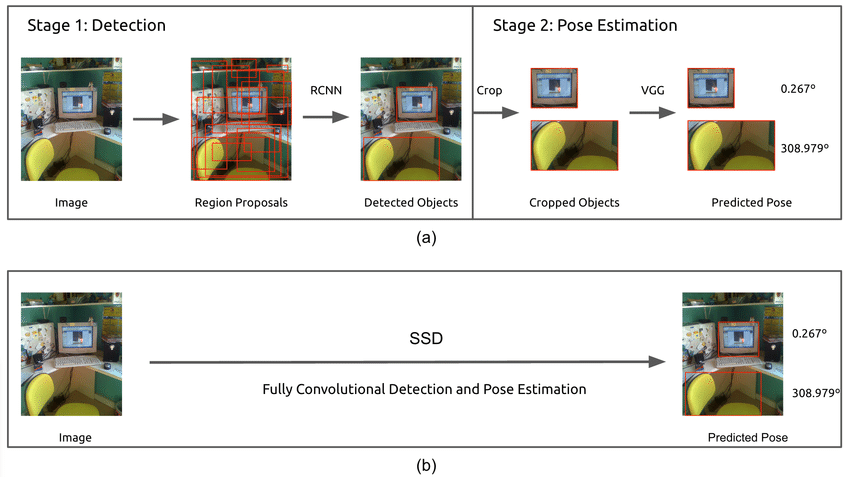
\includegraphics[width=0.7\textwidth]{images/single-vs-two-stage-obj-detector.png}
  \caption{Single vs Two-Stage Object Detection Process}
\end{figure}

\newpage{}
\textbf{Single stage} object detector models processes an image through a
feature extractor using a CNN (Convolutional Neural Network) and then directly
uses the extracted features for classification and regression of bounding boxes.
These models are very fast which is why they are popular for real-time object
detection tasks; however their accuracy performance can sometimes be poor.
Examples of single stage models are SSD, YOLO and RefineDet
(\cite{yoloversionsliterature}.)

\textbf{Two stage} object detector models divides the process into two main
steps. First, it extracts features from the image using a CNN, then selects
regions of interests that will only be used for classification and regression of
bounding boxes. These models are much more accurate than one stage detectors and
are used for tasks where accuracy is prioritized over speed in the medical field
for example RCNN, Fast-RCNN and Faster-RCNN(\cite{singlevstwostagedetectors}).

For the scope of this project, we chose to continue with the YOLO models because
of their speed, their scalability and their lack of computational resources.

We experimented with different versions of the YOLOv5 model, then slowly
levelled up the versions up to version 8.  The YOLOv8 model has been pre-trained
on the COCO (Common Object in Context) dataset, a popular large scale dataset
with 200,000 images across 80 object categories commonly used for benchmarking
computer vision models (\cite{cocodataset}).

We monitored metrics such as mAP (Mean Average Precision), F1-score and the
false positive rate. The figure below shows the metrics of the model as we
iteratively experimented up the version chain.

%model metrics graph
\begin{figure}[htbp]
  \centering
  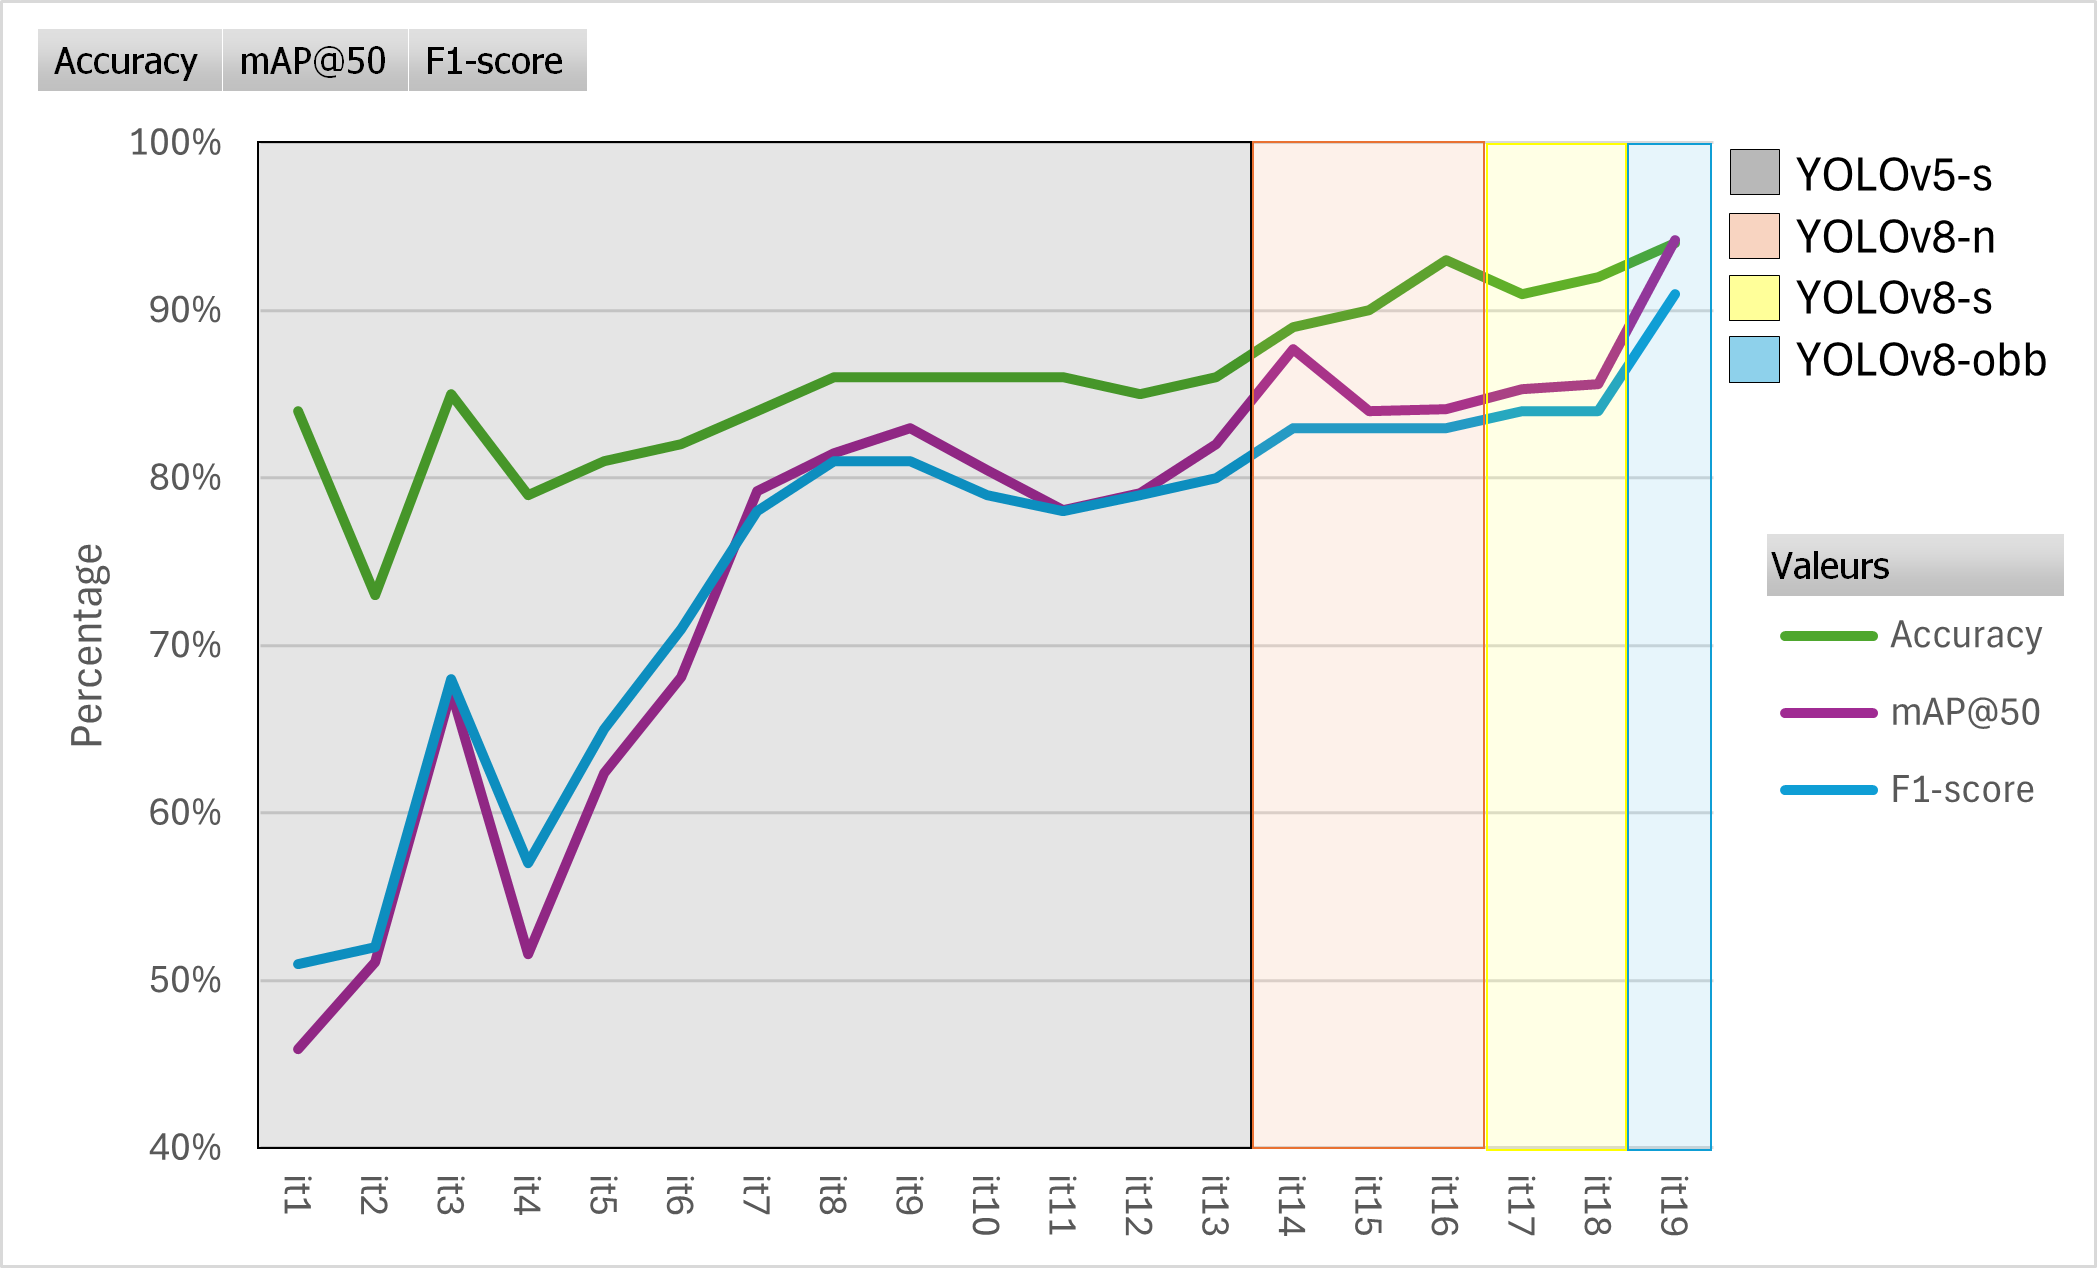
\includegraphics[width=0.85\textwidth]{images/yolo-results.png}
  \caption{YOLO Model training graph}
\end{figure}

We ended the object detection modelling training with the YOLOv8 - Oriented
Bounding Boxes (OBB).
Oriented bounding boxes are a newer type of bounding box where the bounding box
capture the orientation of the object providing a more accurate fit of the
object. They are defined by 5 parameters (center xy, width, height and rotation
angle) and capture the object's spatial orientation more precisely, reducing
overlap and improving the robustness of the object detection model
(\cite{obblit}).

Below you can see the difference in bounding boxes between the labelled image
used for the non-OBB YOLOv5 \& YOLOv8 iterations versus the OBB YOLOv8.

%obb vs non obb bounding boxes
\begin{figure}[htbp]
  \centering
  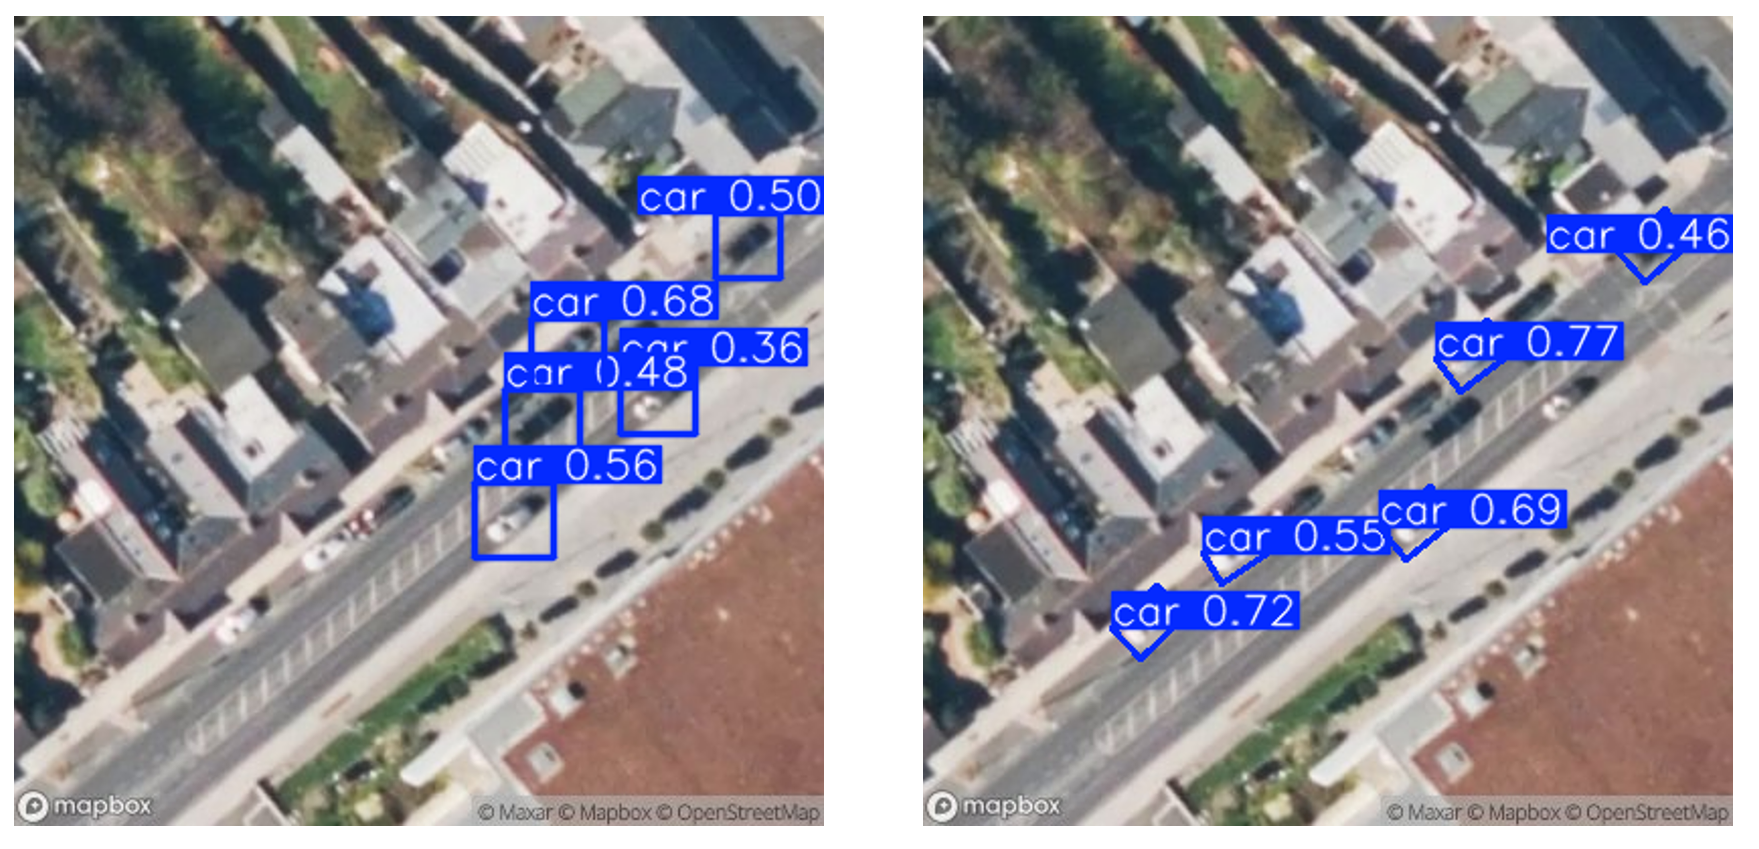
\includegraphics[width=0.85\textwidth]{images/obb-vs-nonobb-img.png}
  \caption{Non-OBB labels (left) versus OBB labels (right)}
\end{figure}

\newpage{}

Thus, the YOLOv8-OBB model was trained on the settings below:

\begin{listing}[htbp]
  \centering
  \begin{minted}{python3}
train_results_obb = yolo8s_obb_model.train(data=data_config,
              epochs=35,
              patience=15,
              optimizer="AdamW",    # Adam + weight decay for less overfitting
              val=True, # validate during training
              seed=1,
              imgsz=416,
              batch=16,
              cache="disk",
              )
  \end{minted}
  \caption{YOLOv8-OBB model training settings}
\end{listing}

The weights of the YOLOv8-OBB model were then saved and used to identify parked
cars on over 18,000 satellite images spanning Dublin City. These images are then
used to identify parking spots.

\subsubsection{Parking spot detection}
Subsequently, to identify the parking spots in each satellite image, the cars
detected by the YOLO model are classified into on the road or parked, based on a
road mask.

\subsubsection{Road mask generation} \label{sec:road_mask_generation} Many
different iterations of the road mask were used, the main iterations and their
differences are explained and showed below in Figure~\ref{fig:mask_iterations}.

The original mask was a very simple binary mask which identified the road pixels
by their color, as the majority of roads were depicted in white and darkened the
rest of the pixels in the image.

Through testing and thoroughly analysing the Mapbox Streets images, motorways
and national roads were discovered to be depicted in yellow or orange.
Therefore, two additional color masks (for orange and yellow) were concatenated
to the original binary mask through bitwise operations.

To refine the mask, and reduce misclassification errors, additional annotations
contained on the Mapbox Streets images such as street names and white dotted
lines which denote a multitude of things (foot paths, planter boxes, pedestrian
crosswalks, football fields delimitations, etc. ) were removed through
morphological operations, leaving only a plain white line for each road. A
number of different kernel sizes, different contour thresholds and other
parameters were tested to achieve the optimal removal of the street names and
additional annotations.

A different approach using Canny Edge Detection was tested, however due to the
nature of the Mapbox Streets images, the edges picked up were not significant
and the overall performances was much worse than the current mask at the time.

\newpage{}

A final improvement to the mask was made to avoid certain misclassification due
to the Mapbox Streets road width not correctly reflecting all the lanes of the
road and therefore classifying on the road cars as parked. This issue was most
prominent for motorways and national roads and was resolved by enlarging those
roads using a dilation technique. Multiple different kernel sizes, different
number of iterations and kernels of different sizes applied consecutively were
tested to find the optimal solution.

\begin{figure}[htbp]
  \centering{}
  \begin{tabular}{cc}
    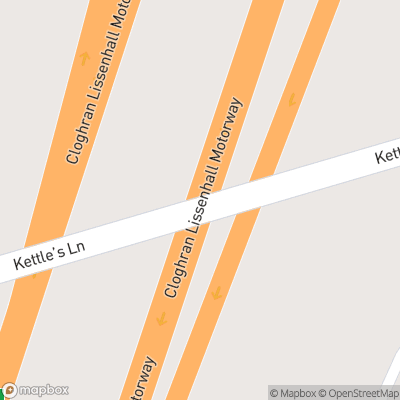
\includegraphics[width=0.30\textwidth]{images/streets.png}  & 
    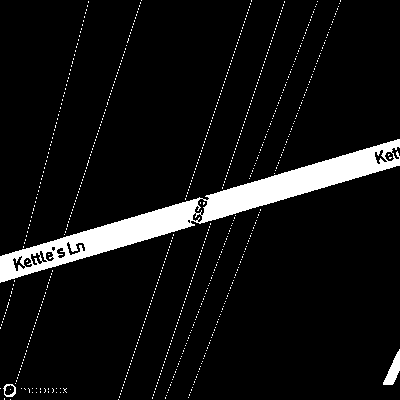
\includegraphics[width=0.30\textwidth]{images/old_mask.png}                             \\
    Mapbox Streets Image                                        & Initial Mask              \\
    
\includegraphics[width=0.30\textwidth]{images/new_mask.png} & 
    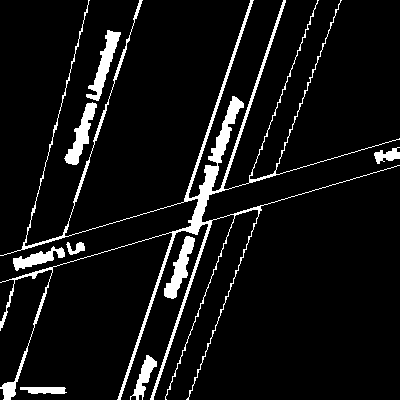
\includegraphics[width=0.30\textwidth]{images/canny_edge_mask.png}                      \\
    Mask with Added Color Masks                                 & Canny Edge Detection Mask \\
    \multicolumn{2}{c}{
\includegraphics[width=0.30\textwidth]{images/current_mask.png}}     \\
    \multicolumn{2}{c}{Current Mask}
  \end{tabular}
  \caption{Different Iterations of the Road Mask}
  \label{fig:mask_iterations}
\end{figure}

\newpage{}

\subsubsection{Classification of cars into on the road or parked}
The cars detected by the Yolo model are then sorted into on the road or parked
based on the road mask previously generated, which is explained in more detail
below.

The model's predictions which are lower than the confidence threshold of 0.4 are
discarded as they are more likely to be misclassifications, such as chimneys or
roof pieces which were often misclassified as cars, which can be seen below on
the second image of Figure~\ref{fig:Road_mask_classification}.

A bounding box for each of the model's predictions is computed from the center
pixel coordinates, the width and the height returned from the model. The overlap
between the bounding box and the road pixels is calculated, and if the overlap
is higher than the threshold of 0.5, the prediction is discarded, keeping only
the parked cars. Different thresholds were tested as well, however overall a
harsher threshold works better given that these detections are used later on for
the empty parking detection.

For each of the model's predictions for parked cars, the center pixels
coordinates are mapped to geographic coordinates (longitude and latitude), and
the width, height, rotation and orientation based on the angle are saved. The
horizontal orientation is assigned for spots that have a rotational angle in
degrees ranging between -45 and 45 or between 135 and 225, while the vertical
orientation is assigned to the remaining spots that do not fit the criteria.

For testing and debugging purposes, all the bounding boxes of the cars found by
the model are drawn onto the satellite image, on the road cars are drawn in blue
while parked cars are drawn in red as seen below in
Figure 21.

\begin{figure}[htbp]
  \centering
  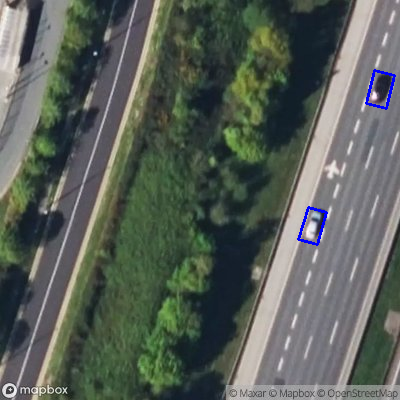
\includegraphics[width=0.30\textwidth]{images/road_mask_classification1.png}
  \hfill
  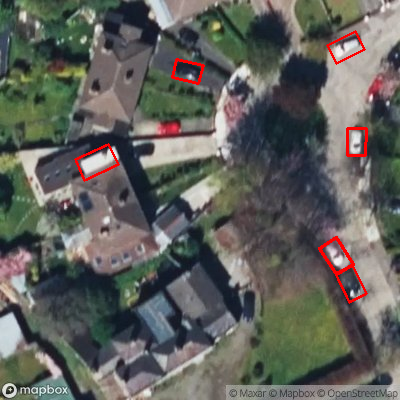
\includegraphics[width=0.30\textwidth]{images/road_mask_classification2.png}
  \hfill
  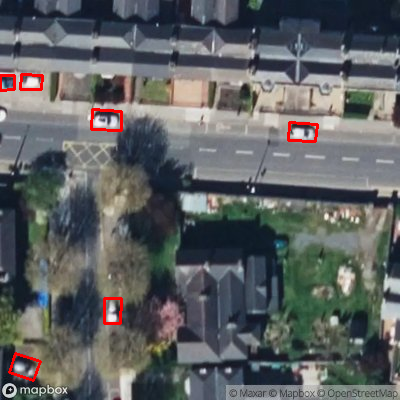
\includegraphics[width=0.30\textwidth]{images/road_mask_classification3.png}
  \caption{Classification of cars as on the road or parked: (left) Initial Classification, (center) Intermediate Stage, (right) Final Classification.}
  \label{fig:road_mask_classification}
\end{figure}


\newpage

\subsubsection{Empty parking spot detection}
Subsequently, empty parking spots are detected between parked cars in each
image, based on the parked cars detected by the Yolo model and classified using
the road mask. Originally 4 cases were considered, cars parked horizontally in a
row or in a column, cars parked vertically in a column and cars parked
vertically side by side. However horizontally parked in a column and vertically
parked side by side were removed as they lead to too many misclassifications,
namely the vertically parked side by side lead to adding many additional cars in
driveways in residential areas.\\
A number of different variations and calculation techniques were tested out,
however only the final version will be explained below.

Average parking spot width and length in pixels are calculated for each image,
to draw the empty spots more uniformly. Average parking spot width and length in
meters are set to 3.05 as found to be the optimal value through testing
accounting for the variations in size. Setting this value avoids
misclassifications as previously the average width and length in meters were
calculated dynamically, however in cases where the averages were lesser than 3,
spots tended to overlap.

The parked cars detected are then sorted by latitude for horizontally aligned
cars and by longitude for vertically aligned cars, to identify gaps between
consecutive cars. For each pair of consecutive spots, the distance in meters in
between them is calculated. The gap is adjusted to account for the half cars on
both sides, as the coordinates of the parked car represent the center of the
car. For the gaps smaller than the maximum gap threshold of 12 meters and larger
than the average size of a car, where there is enough space to fit 1 or more
car, and where the angle deviation is smaller than a threshold of 35 degrees, to
ensure the spots are sufficiently aligned, the number of cars that fit into the
gap is calculated. Based on the number of empty spots found, the coordinates for
those empty spots are calculated to be aligned with the 2 consecutive cars and
then added to a list of empty spots detected.

Afterwards, duplicate spots defined as spots that overlap too much and where the
distance between 2 spots is smaller than a threshold of 1 meter are removed. As
well, spots coinciding with cars identified by the Yolo model, where the
distance between them is smaller than 1.25 meters are removed from the empty
spots found. Subsequently, empty spots that overlap with the road are filter out
in a similar manner to the classification done by the road mask.

Following the detection of all the empty spots, the bounding boxes corresponding
to each spot are drawn onto the satellite image in green as shown in
Figure 22.

\begin{figure}[htbp]
  \centering
  \begin{minipage}{0.45\textwidth}
    \centering
    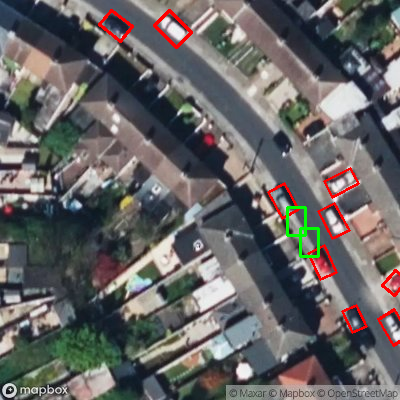
\includegraphics[width=\textwidth]{images/empty_parking1.png}
  \end{minipage}
  \hfill
  \begin{minipage}{0.45\textwidth}
    \centering
    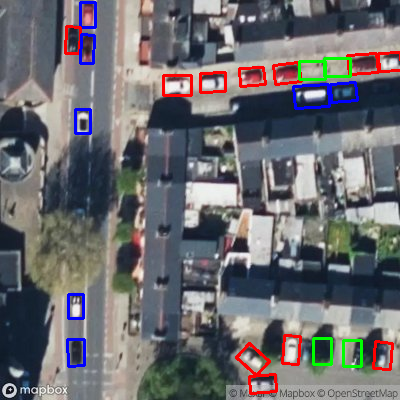
\includegraphics[width=\textwidth]{images/empty_parking2.png}
  \end{minipage}
  \hfill
  \begin{minipage}{0.45\textwidth}
    \centering
    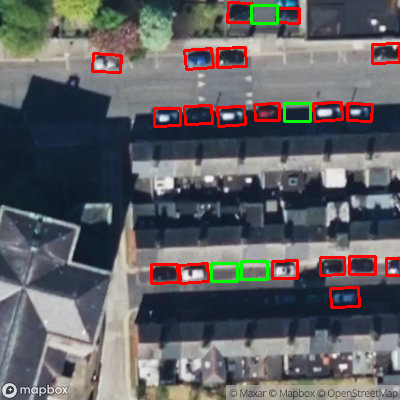
\includegraphics[width=\textwidth]{images/empty_parking3.png}
  \end{minipage}
  \hfill
  \begin{minipage}{0.45\textwidth}
    \centering
    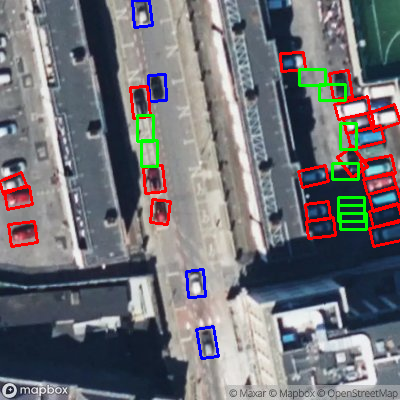
\includegraphics[width=\textwidth]{images/empty_parking4.png}
  \end{minipage}
  \caption{Empty Parking Spot Detection}
  \label{fig:Empty_parking_detection}
\end{figure}

\newpage

\subsubsection{Classification of all spots detected}
All the parking spots detected, including the parked cars identified by the
model and the empty parking spots are then classified into 3 different classes:
public (on the street parking), private (residential parking) and parking lot,
based on their proximity to the nearest road.

Multiple different clustering approaches were tested out to cluster spots
together, such as DBSCAN, HDBSCAN and OPTICS. Overall DBSCAN performed the best
and the quickest out of all the clustering algorithms, given that some images
contained very few parking spots, meaning clustering was only significant in
cases with a minimum number of parking spots. Through testing, the optimal
hyperparmeters found for DBSCAN are \texttt{eps} : 55 and \texttt{min\_samples}
: 5, which allow the correct identification of the clusters, avoiding
misclassifications of residential areas with many cars as parking lots, which
was a common misclassification initially, when the hyperparameters and
thresholds were not set correctly.\\
\texttt{eps} refers to the maximum distance between two points for them to be
considered as neighbors and \texttt{min\_samples} refers to the minimum number
of points required to form a cluster.\\
Using HDBSCAN and OPTICS required a minimum number of samples larger or equal to
2, however given that not all images necessarily contained at least 2 parked
cars (some images may contain only on the road cars for example), clustering
using those algorithms was not possible in all cases, therefore -1 was assigned
to the spots belonging to no clusters similarly to the default behaviour of
DBSCAN. Clustering using HDBSCAN gave similar results to DBSCAN, however not as
good, while OPTICS only found smaller clusters which were not as significant and
not particularly helpful to subsequently classify the spots into the parking lot
category.

Parking spots are classified as public if the proximity to the nearest road is
less than a pixel threshold of 30, otherwise the parking spots are considered
private. This optimal threshold was found through extensive testing on a test
set containing various edge cases. Parking spots are classified as parking lots,
when clusters of 18 or more spots are identified in an image. Larger clusters
are prioritized as parking lots containing less spots are not as relevant to the
target user and given that the threshold of 18 spots minimizes the risk of
misclassifying residential areas as parking lots.

Afterwards, clusters and classification labels are drawn onto the satellite
image. The clusters are color coded and denoted as a circle at the center of the
bounding box, while the classification label is written to the right of the
bounding box. The private class in written in red, public in green and parking
lot in white as seen below in Figure 23.

\begin{figure}[htbp]
  \centering
  \begin{minipage}{0.45\textwidth}
    \centering
    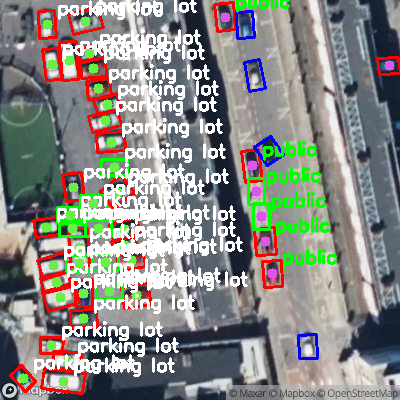
\includegraphics[width=\textwidth]{images/classification1.png}
  \end{minipage}
  \hfill
  \begin{minipage}{0.45\textwidth}
    \centering
    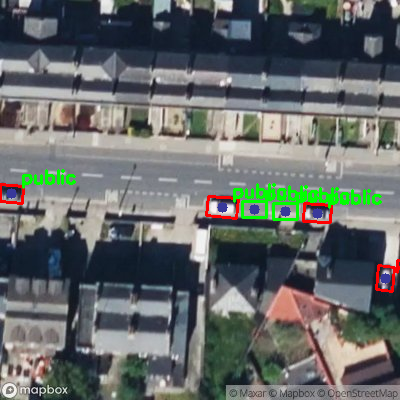
\includegraphics[width=\textwidth]{images/classification2.png}
  \end{minipage}
  \hfill
  \begin{minipage}{0.45\textwidth}
    \centering
    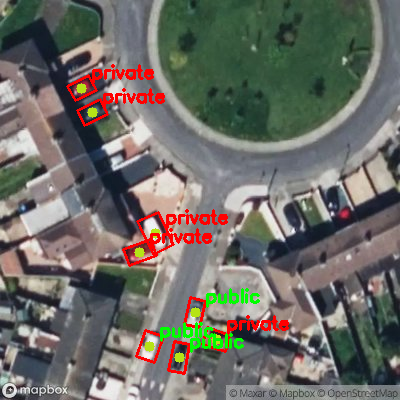
\includegraphics[width=\textwidth]{images/classification3.png}
  \end{minipage}
  \hfill
  \begin{minipage}{0.45\textwidth}
    \centering
    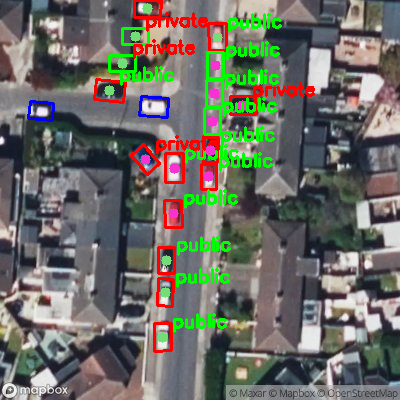
\includegraphics[width=\textwidth]{images/classification4.png}
  \end{minipage}
  \caption{Classification of all spots into private, public and parking lot}
  \label{fig:classification_all_spots}
\end{figure}

\newpage

\subsubsection{Uploading points to the backend server}
The longitude, latitude and classification of all the parking spots detected are
then saved to a csv file. Potential spot duplicates are dropped, as the same car
may be in multiple images given that the images are defined by their center
coordinates, which causes adjacent images to overlap and share common areas. The
rightmost part of one image can overlap with the leftmost part of another image.

Subsequently, the parking zones and costs associated to each parking spot found
are added to the csv file. Dublin City Council defines different parking zones
by color, based on their high to moderate demand which changes the price per
zone as seen below in Figure 24.

\begin{figure}[htbp]
  \centering
  \begin{minipage}{0.45\textwidth}
    \centering
    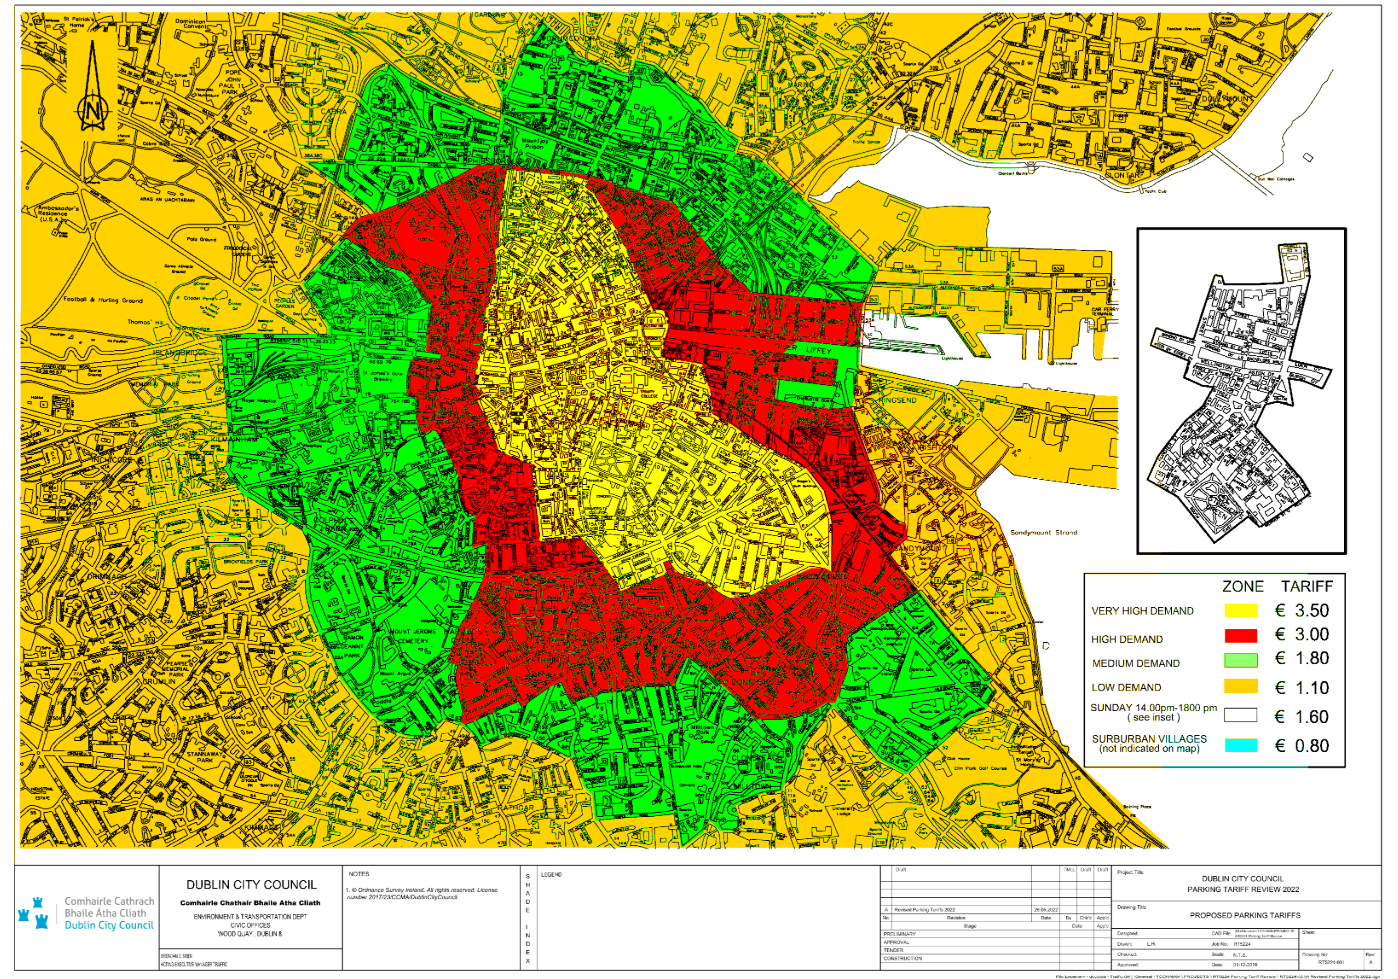
\includegraphics[width=\textwidth]{images/Parking_zones_map.png}
  \end{minipage}
  \hfill
  \begin{minipage}{0.45\textwidth}
    \centering
    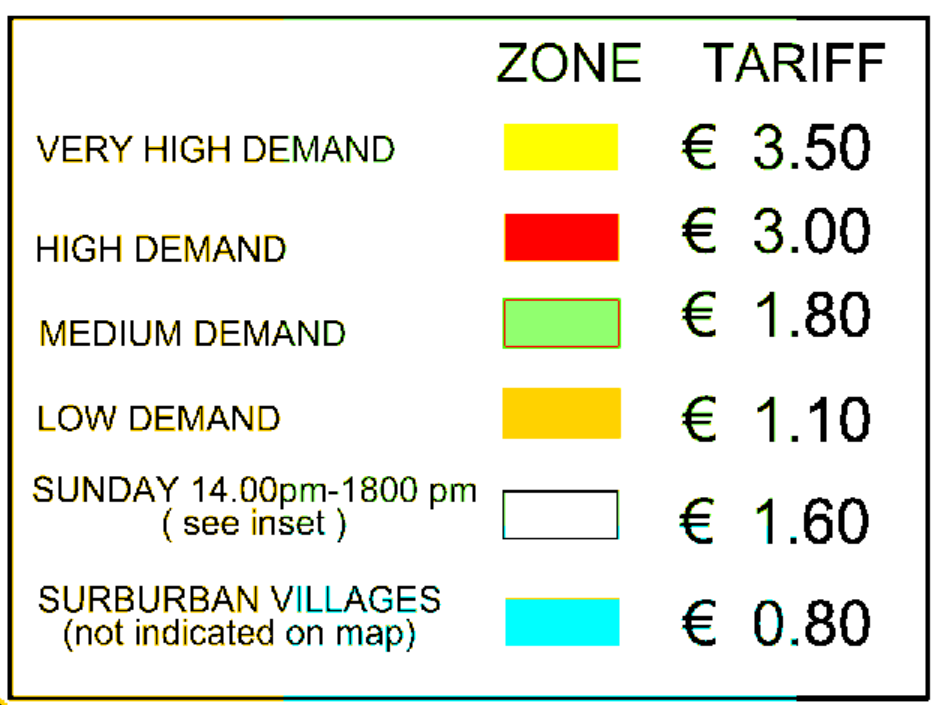
\includegraphics[width=\textwidth]{images/Parking_zones_cost.png}
  \end{minipage}
  \caption{Parking zones and cost defined by Dublin City Council}
  \label{fig:Parking_zones}
\end{figure}

The csv file containing the longitude, latitude, classification label, parking
zone and parking cost is then uploaded to the PostgreSQL database, in the
backend server using the \texttt{send\_points.py} script.

\subsection{Summary of main challenges}
Throughout the implementation of our technical solution, there have been many
major challenges and changes which will be discussed in this section.


The biggest initial hurdle was finding a labelling software to annotate our
satellite images. Initially, we had settled on LabelImg, however it was no
longer being supported on most of our operating systems and was crashing on
launch. Instead, we turned towards Label Studio and the ML Backend extension, we
had intended on using for its active learning functionality that would have
enabled using Yolo v5 to automatically label our training images, after only
annotating a few images. After much troubleshooting, we decided to switch
approaches to manually label the images and subsequently train the Yolo model on
those images.

The next challenge related to training the YOLO model to identify cars on the
satellite images. An object detection model remains a deep neural network model,
which is computationally intensive the more complex it becomes.

We were limited in our training of the model due to limitations in available
computational resources. Tuning for 35 iterations would last several hours, and
training above a certain number of epochs would not yield better results.
Training the model was both computationally expensive and very time consuming.
Another challenge referred to the low resolution of the satellite images,
heavily contributing the high misclassification rate in the early beginnings of
model training. We managed to stabilised that through proper model choosing and
tuning however, the biggest factor contributing to the remaining false positive
rate is the low number of training data.

Ideally we would've preferred to have at least 500 training images, however due
to time constraints we settled on half of that, and compensated by putting a
higher confidence threshold than the one dictated by the F1-curve.

Another major challenge, was the empty parking detection section. The crucial
decisions and changes are recounted below, following the timeline of our
project: \\
In Week 8, the \texttt{parking\_detection.py} script was updated to use the most
up to date trained Yolo model, Yolo v8 obb, that returned oriented bounding
boxes, causing many issues in the version of our script at the time,
specifically the way of access the bounding boxes predicted by the model had
changed. Furthermore, given the change to oriented bounding boxes, the size of
the bounding boxes became more variable, which allowed the script to be adapted
to use average parking spot dimensions.\\
Week 9 was decisive in implementing a double passthrough to sort the cars by
longitude and the latitude to identify both the horizontal and vertical spots.
Moreover, the \texttt{parking\_detection.py} script was updated to use the
xywhr(centre coordinates, width, height and rotation) bounding boxes instead of
the xyxy (top left, bottom right)  bounding boxes we were using initially. This
major change was crucial and allowed for more modularity and allowed the
separation into horizontal and vertical cases in a more consistent manner. As
well many additional improvement were made that week, such as the removal of
overlapping spots and filtering out the empty spots detected on the road.\\
In week 12, the empty parking detection was completely finalized, resolving the
majority of the outstanding issues. The 2 cases causing too many false positives
were removed and the condition on the angle alignment was refined and added.

Another major issue was the selection and accurate labelling of the test sets to
evaluate each subpart of our model. Week 11 marked the beginning of the empty
parking detection evaluation. Labelling the test set accurately was a big
challenge, many different phases of relabelling and improvements occurred, to
ensure the maximum overlap between the true labels and the predictions and
achieve a high enough IoU. During Week 12, the 2 other evaluation scripts were
finalized. Similarly, multiple phases of labelling and relabelling happened. For
the classification of spots evaluation, additional images needed to be added to
the test set for the private class, as the lack of enough instances was making
that class perform much more poorly in comparison to the other classes.

\subsubsection{Evaluation of each submodule of the parking detection model}
Each major section of the parking detection model was evaluated individually in order to assess the overall performance. The results will be presented for each section below.

\subsubsection{Evaluation of the YOLOv8-OBB model}
The YOLOv8-OBB model was evaluated on a validation set of 51 images, where precision, recall, accuracy, mean average precision (mAP@50) and F1-score were computed. These were the scores below:
%yolov8 obb results
\begin{table}[htbp]
  \centering
  \begin{tabular}{|p{0.18\textwidth}|p{0.1\textwidth}|p{0.1\textwidth}|p{0.1\textwidth}|p{0.1\textwidth}|p{0.1\textwidth}|p{0.12\textwidth}|}
    \hline
    \textbf{Model} & \textbf{Accuracy} & \textbf{Precision} & \textbf{Recall} & \textbf{F1-score} & \textbf{mAP@50} & \textbf{Confidence threshold} \\
    \hline
    YOLOv8-OBB     & 94\%              & 100\%              & 99\%            & 91\%              & 94\%            & 35\%                          \\
    \hline
  \end{tabular}
  \caption{YOLOv8-OBB model results}
\end{table}\\

The model obtains near perfect precision and recall on the validation data set meaning it is very good at correctly identifying the majority of true positives and preventing false positives.
However, the lower f1 score of 91\% highlights the slight imbalance between precision and recall. Additionally, the confidence threshold is based on the F1-score, suggesting that the model performs at a level where precision and recall are balanced best closer to 30\%. This indicates that our model is not strict.

Although the overall metrics obtained are quite high, it is important to consider that, the validation and training data are not very large, therefore impacting overall model performance to identify cars in a larger detection set.

\subsubsection{Evaluation of the classification of cars into on the road or parked}
The classification of cars into on the road or parked by the road mask is evaluated in the \texttt{evaluate\_road\_mask.py} Python script.
The classification is evaluated on the following metrics commonly used for object detection tasks: Average Intersection over Union (IoU), Balanced Accuracy and Precision, Recall, F1 Score, Accuracy, Specificity per class.

These metrics are defined in detail as follows.

The IoU is calculated as the overlap between the predicted bounding box \( B_p \) and the ground truth bounding box \( B_g \), divided by their union:

\[
  \text{IoU} = \frac{|B_p \cap B_g|}{|B_p \cup B_g|}
\]

The Average IoU is defined as the mean IoU across all detections:

\[
  \text{Average IoU} = \frac{1}{N} \sum_{i=1}^{N} \text{IoU}_i
\]

where \( N \) is the total number of detections.

Precision is defined as the ratio of true positives (TP) and the sum of true positives and false positives (FP):

\[
  \text{Precision} = \frac{\text{TP}}{\text{TP} + \text{FP}}
\]

Recall is defined as the ratio of true positives (TP) and the sum of true positives and false negatives (FN):

\[
  \text{Recall} = \frac{\text{TP}}{\text{TP} + \text{FN}}
\]

The F1 Score is defined as the harmonic mean of precision and recall:

\[
  \text{F1 Score} = 2 \cdot \frac{\text{Precision} \cdot \text{Recall}}{\text{Precision} + \text{Recall}}
\]

Accuracy is defined as the proportion of correct predictions (TP and TN) out of all the predictions:

\[
  \text{Accuracy} = \frac{\text{TP} + \text{TN}}{\text{TP} + \text{TN} + \text{FP} + \text{FN}}
\]

Balanced Accuracy is defined as the average of Sensitivity (or Recall) and Specificity:

\[
  \text{Balanced Accuracy} = \frac{\text{Sensitivity} + \text{Specificity}}{2}
\]

where:
\[
  \text{Sensitivity/Recall} = \frac{\text{TP}}{\text{TP} + \text{FN}}, \quad
  \text{Specificity} = \frac{\text{TN}}{\text{TN} + \text{FP}}
\]

These metrics are then saved in a csv file for each test image as well as the overall average metrics on the entire test set.

A test set of 50 images was carefully selected to include edge cases and difficult cases and then consistently labelled in Label Studio as seen in Figure~\ref{fig:LabelStudio_test_set}. The labels are drawn without rotation to ensure the maximum overlap, as the labels are exported to \texttt{txt} format and include only the pixel coordinates, width and  height of the bounding boxes annotated.

\begin{figure}[htbp]
  \centering
  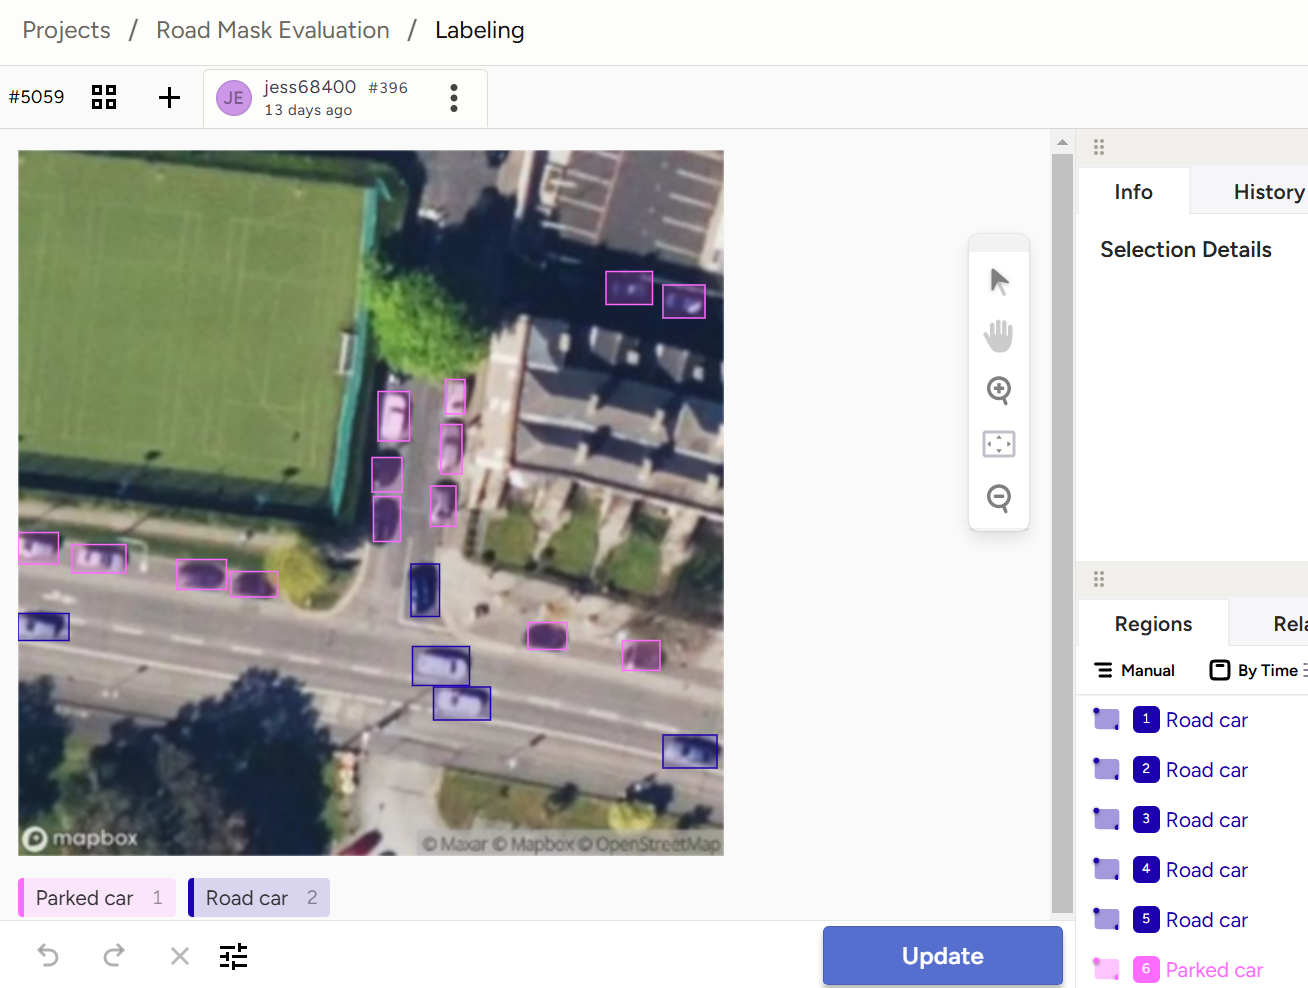
\includegraphics[width=0.9\textwidth]{images/label_studio4.png}
  \caption{Road mask classification test set images being annotated in Label Studio}
  \label{fig:LabelStudio_test_set}
\end{figure}

\newpage{}


The overall results on test set are presented below in Table~\ref{tab:metrics1}.

\begin{table}[htbp]
  \centering
  \begin{tabular}{|l|c|c|}
    
    \hline
    \textbf{Metric}           & \textbf{Parked} & \textbf{Road} \\ \hline
    Average IoU               & 0.66            & 0.66          \\ \hline
    Average Balanced Accuracy & 0.58            & 0.58          \\ \hline
    Average Precision         & 0.70            & 0.90          \\ \hline
    Average Recall            & 0.75            & 0.67          \\ \hline
    Average F1 Score          & 0.59            & 0.54          \\ \hline
    Average Accuracy          & 0.69            & 0.64          \\ \hline
    Average Specificity       & 0.74            & 0.79          \\ \hline
  \end{tabular}
  \caption{Performance Metrics for Road Mask Classification}
  \label{tab:metrics1}
\end{table}

Precision and Recall are relatively high for both classes. Precision for the on the road cars class is extremely high as the majority of the cars in the test set were perfectly horizontally or vertically aligned, and given that the rotation cannot be exported in label studio, the bounding box is drawn less accurately unless if it is perfectly horizontally or vertically aligned.

\newpage{}

The majority of papers available, that explore object detection for cars on satellite images, evaluate their experiment on more general metrics such as Average Precision (AP) and Mean Average Precision (mAP). AP represents the area under the precision-recall curve and mAP represents the mean of the APs across all the different classes. These metrics provide a broader overview of the model's performance as it is measured across varying thresholds.
Therefore the results obtained are not as comparable, given that precision, recall and f1 score are calculated for a fixed IoU threshold in our evaluation.
Finding the optimal fixed threshold was opted for to find the most accurate detections, as those detections are used later on for the classification of the spots into public, private and parking lot.

The results achieved, presented above in Table~\ref{tab:metrics1}, are in line with \cite{similarresults}, who achieve a precision of 0.75, a recall of 0.66 and an f1 score of 0.7 at the IoU threshold of 0.3, for detecting parked car on stereo satellite images.

The current road mask has a few outstanding problems, that are discussed further below.\\
Firstly, sometimes not all parts of the street names are completely removed due to the watermark at the bottom of the image or in the case of the street name being on the very edge of the image. However this seems to rarely be the cause of misclassifications.\\
For streets where the street name takes up all the whole width of the street, the area where the street name is written is completely erased, which can cause cars on the road to be misclassified as parked.\\
A key issue, previously discussed in Section~\ref{sec:road_mask_generation}, is that the Mapbox Streets images do not correctly reflect the width of the road for roads with multiple lanes, which leads to cars on the road being misclassified as parked for the furthest out lanes.
This issue was resolved for motorways as those roads are depicted in orange or yellow, therefore it was possible to distort the road on the mask to cover more surface. However doing this for the regular roads, would cause far more misclassifications, then fix the current ones.\\
Another problem that is inherently due to the Mapbox Streets images is the Dublin Tunnel being marked on the images making it appear above ground even though it is underground, which leads to misclassiifcations in that specific area.

Some images from the test set can be seen below, in Table~\ref{tab:test_images1}.
The predicted parked cars are drawn in red while the true labels are drawn in light pink. The predicted on the road cars are drawn in blue while the true labels are drawn in cyan.

\begin{table}[htbp]
  \centering
  \begin{tabular}{cc}
    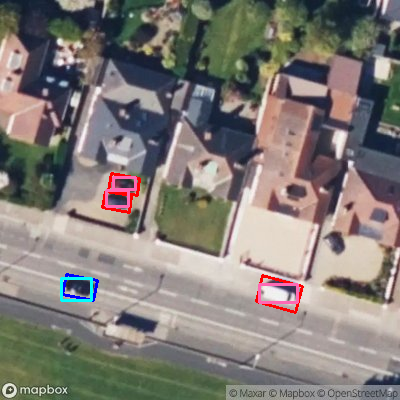
\includegraphics[width=0.4\textwidth]{images/image1_road_mask_classification_test_set.png} & 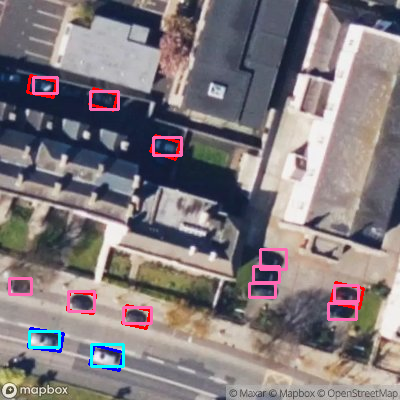
\includegraphics[width=0.4\textwidth]{images/image2_road_mask_classification_test_set.png} \\
    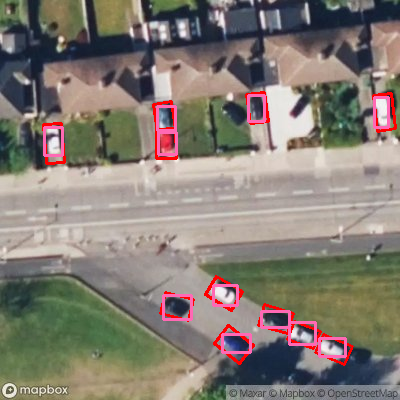
\includegraphics[width=0.4\textwidth]{images/image3_road_mask_classification_test_set.png} & 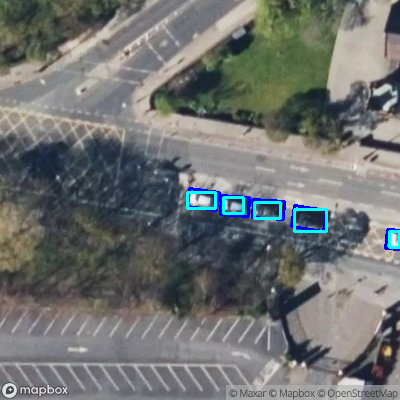
\includegraphics[width=0.4\textwidth]{images/image4_road_mask_classification_test_set.png} \\
    \multicolumn{2}{c}{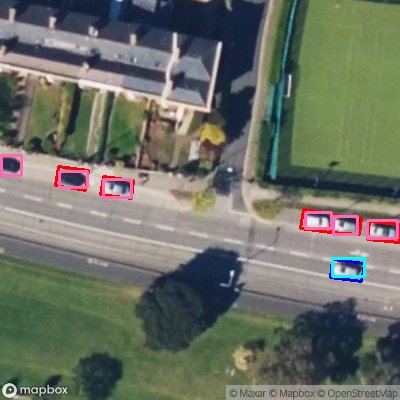
\includegraphics[width=0.4\textwidth]{images/image5_road_mask_classification_test_set.png}}                                                                          \\
  \end{tabular}
  \caption{Images from the Road Mask Classification Test Set}
  \label{tab:test_images1}
  
\end{table}

\newpage{}

\subsubsection{Evaluation of the empty parking detection}
The empty parking detection logic is evaluated in the \texttt{evaluate\_empty\_parking\_detection.py} Python script.
The classification is evaluated on the following metrics: Average IoU, Average Precision, Average Recall, Average F1 Score, Average Orientation Accuracy, Average Spot Detection Ratio (SDR), Average Spot Detection Error (SDE), Average False Positive Rate (FPR), and Average False Negative Rate (FNR).

The additional metrics are defined as follows.

The Average Orientation Accuracy is defined as the ratio of the number of predictions that correctly identify the orientation (either horizontal or vertical) of the spots on the total number of true spots:

\[
  \text{Average Orientation Accuracy} = \frac{\text{Correct Orientation Predictions}}{\text{Total True Labels}}
  = \frac{N_{\text{correct\_orientation}}}{N_{\text{true\_labels}}}
\]

where \( N_{\text{correct\_orientation}} \) represents the number of predictions with correct orientation, and \( N_{\text{true\_labels}} \) represents the total number of true labels.

The Spot Detection Ratio is defined as the ratio of the number of predictions and the total number of true labels:

\[
  \text{SDR} = \frac{N_{\text{predictions}}}{N_{\text{total\_true\_labels}}}
\]

where \( N_{\text{predictions}} \) is the total number of detected spots, and \( N_{\text{total\_true\_labels}} \) is the total number of true labels.

The Spot Detection Error is defined as the absolute difference between the number of predictions and the total number of true labels:

\[
  \text{SDE} = |N_{\text{predictions}} - N_{\text{total\_true\_labels}}|
\]

The False Positive Rate is defined as the proportion of incorrectly predicted positives (FP) out of all the actual negatives:

\[
  \text{Average FPR} = \frac{\text{FP}}{\text{FP} + \text{TN}}
\]

The False Negative Rate is defined as the proportion of incorrectly predicted negatives (FN) out of all the actual positives:

\[
  \text{Average FNR} = \frac{\text{FN}}{\text{TP} + \text{FN}}
\]

These metrics are then saved in a csv file for each test image as well as the overall average metrics on the entire test set.

Likewise a test set of 50 images was carefully selected and consistently labelled in Label Studio, without rotation to ensure the maximum overlap. The pixel coordinates, width and height of the annotated bounding boxes are exported. The orientation of each bounding box, is calculated automatically in the evaluation script when loading in the true labels.\\
Achieving a high IoU was a significant challenge, specifically in this section of the model, as the positioning of the spots can be difficult to label accurately. Indeed, it was difficult to identify if there was sufficient space available to fit a car.
To remedy this issue, the IoU threshold was lowered to 0.35, as there was still significant overlap visible when analysing the test images.
The problems linked to the overlap, is equally due to the differences in orientation as the true labels and the predictions are calculated differently.
For the true labels, the orientation is based on whether the width or length of the spot is larger (the spots with larger width are labelled as horizontal and the spots with larger length are labelled as vertical), while for the model's predictions the orientation is based on the angle measurement.

The overall results on test set are presented below in Table~\ref{tab:metrics2}.


\begin{table}[htbp]
  \centering
  \begin{tabular}{|l|c|}
    \hline
    \textbf{Metric}                    & \textbf{Value} \\ \hline
    Average IoU                        & 0.59           \\ \hline
    Average Precision                  & 0.77           \\ \hline
    Average Recall                     & 0.70           \\ \hline
    Average F1 Score                   & 0.69           \\ \hline
    Average Orientation Accuracy       & 0.64           \\ \hline
    Average Spot Detection Ratio (SDR) & 1.05           \\ \hline
    Average Spot Detection Error (SDE) & 1.44           \\ \hline
    Average False Positive Rate (FPR)  & 0.23           \\ \hline
    Average False Negative Rate (FNR)  & 0.22           \\ \hline
  \end{tabular}
  \caption{Performance Metrics for Empty Parking Detection}
  \label{tab:metrics2}
\end{table}


The Average Orientation Accuracy being somewhat low of only 0.64, is expected as the orientation labels for the test set are calculated automatically based on the width and length of the bounding box, while the orientation associated with the model’s prediction is based on the rotation. This is visible in images 1 and 3 of Table~\ref{tab:test_images2}.

The results achieved, presented above in Table~\ref{tab:metrics2}, are similar to other articles performing car detection on satellite imagery such as \cite{similarresults}.

The main reason empty parking spots are not detected is due to the fact that cars are classed as on the road by the road mask, therefore given that the empty parking detection logic only fills in gaps between parked cars it cannot find the empty spots, as seen in the bottom left of the second image of Table~\ref{tab:test_images2}.
Additionally, due to the misclassifications of chimneys or roof pieces as cars by the Yolo model, additional empty spots that should not be identified are detected, as seen on the left of the third image of Table~\ref{tab:test_images3}.
Furthermore, some spots are too small to be found by the model given the threshold set for the average width and average height.\\
Other minor issues that sometimes lead to empty parking spots not being detected are due to angle misalignment, when one car is oriented incorrectly and more slanted, leading to the angle between the 2 cars being larger that the threshold or when 2 cars are too far apart to fill in the gap.

A few images from the test set are displayed below, in Table~\ref{tab:test_images2}.
The predicted empty parking spots are drawn in green while the true labels are in light pink.

\begin{table}[htbp]
  \centering
  \begin{tabular}{cc}
    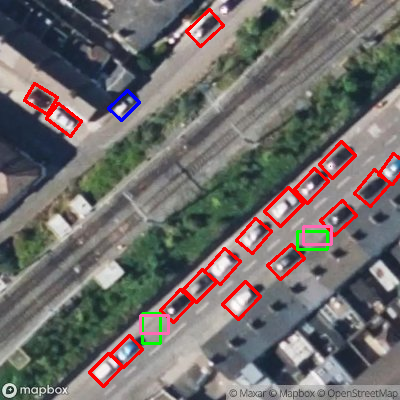
\includegraphics[width=0.4\textwidth]{images/image1_empty_parking_detection_test_set.png} & 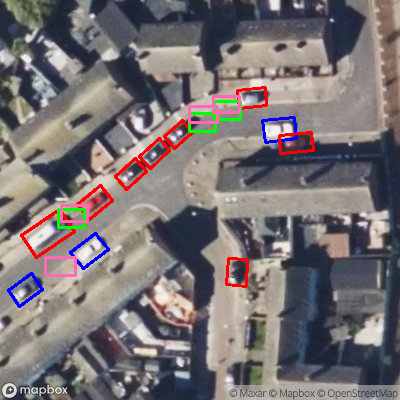
\includegraphics[width=0.4\textwidth]{images/image2_empty_parking_detection_test_set.png} \\
    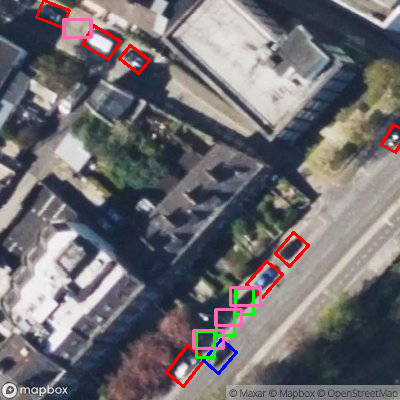
\includegraphics[width=0.4\textwidth]{images/image3_empty_parking_detection_test_set.png} & 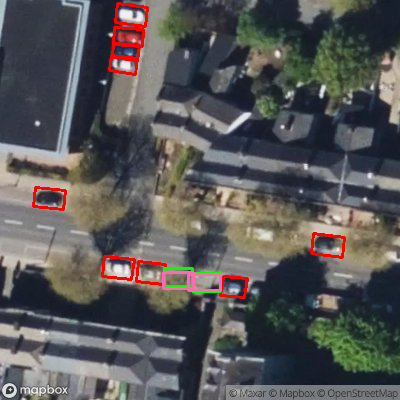
\includegraphics[width=0.4\textwidth]{images/image4_empty_parking_detection_test_set.png} \\
    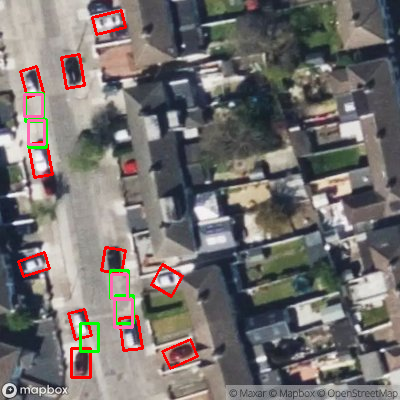
\includegraphics[width=0.4\textwidth]{images/image5_empty_parking_detection_test_set.png} & 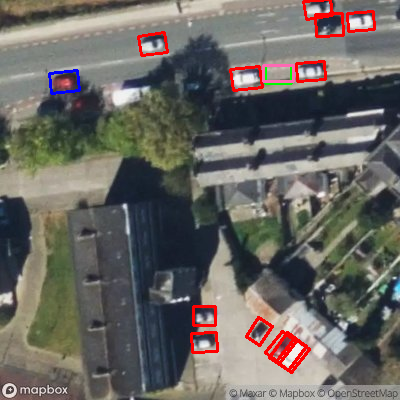
\includegraphics[width=0.4\textwidth]{images/image6_empty_parking_detection_test_set.png} \\
  \end{tabular}
  \caption{Images from the Empty Parking Detection Test Set}
  \label{tab:test_images2}
\end{table}

\newpage{}

\subsubsection{Evaluation of the classification of the spots detected into private, public and parking lot}
The classification of the spots detected into private, public and parking lot is evaluated in the \texttt{evaluate\_classification\_of\_spots.py} Python script.
The classification is evaluated on the following metrics as defined previously: Average IoU, Balanced Accuracy and Precision, Recall, F1 Score, Accuracy, Specificity per class. These metrics are saved in a csv file for each test image as well as the overall average metrics on the entire test set.

Similarly, a test set of 50 images was carefully selected and consistently labelled in Label Studio, without rotation to ensure the maximum overlap.

The overall results on test set are presented below in Table~\ref{tab:metrics3}.

\begin{table}[htbp]
  \centering
  \begin{tabular}{|l|c|c|c|}
    \hline
    \textbf{Metric}           & \textbf{Public} & \textbf{Private} & \textbf{Parking Lot} \\ \hline
    Average IoU               & 0.60            & 0.60             & 0.60                 \\ \hline
    Average Balanced Accuracy & 0.57            & 0.57             & 0.57                 \\ \hline
    Average Precision         & 0.73            & 0.65             & 0.59                 \\ \hline
    Average Recall            & 0.72            & 0.75             & 0.74                 \\ \hline
    Average F1 Score          & 0.68            & 0.62             & 0.61                 \\ \hline
    Average Accuracy          & 0.67            & 0.54             & 0.63                 \\ \hline
    Average Specificity       & 0.59            & 0.54             & 0.41                 \\ \hline
  \end{tabular}
  \caption{Performance Metrics for Parking Spot Classification}
  \label{tab:metrics3}
\end{table}

The performance is similar for all 3 classes, however for the parking lot class more false positives are present, given that having many bounding boxes clustered together creates more unpredictability adding more additional spots.

The results achieved, presented above in Table~\ref{tab:metrics3}, are in line with other articles performing car detection on satellite imagery such as \cite{similarresults}.

The main outstanding problem for this section is residential areas which are very rarely misclassified as parking lots.
Additionally, in cases where public spots are quite far from the nearest road, the spots are misclassified as private, which is not a major issue.\\
Another point worth noting is that smaller parking lots with less than 18 spots are not detected though that is intentional and by design in order to focus on larger parking lots and avoid misclassifications.

A few images from the test set are shown below, in Table~\ref{tab:test_images3}.
The predicted public spots are drawn in green while the true labels are in dark green. The predicted private spots are highlighted in red while the true labels are in light pink. The predicted parking lot spots are shown in blue while the true labels are in cyan.

\begin{table}[htbp]
  \centering
  \begin{tabular}{cc}
    \includegraphics[width=0.4\textwidth]{images/image1_classification_test_set.png} & \includegraphics[width=0.4\textwidth]{images/image2_classification_test_set.png} \\
    \includegraphics[width=0.4\textwidth]{images/image3_classification_test_set.png} & \includegraphics[width=0.4\textwidth]{images/image4_classification_test_set.png} \\
    \includegraphics[width=0.4\textwidth]{images/image5_classification_test_set.png} & \includegraphics[width=0.4\textwidth]{images/image6_classification_test_set.png} \\
  \end{tabular}
  \caption{Images from the Parking Spot Classification Test Set}
  \label{tab:test_images3}
\end{table}

\newpage{}

\subsection{Frontend}
In the future, one of the major focuses on the frontend development of Magpie will be the implementation of user feedback and the improvement of the look and feel of the platform. The current interface provides a great skeleton, but user interaction throughout the platform and accuracy of data displayed need a little more work.




\subsection{Backend}
\subsubsection{Application Security}
\textbf{Fix Issues with JWTs}\\
As mentioned in the discussion of JSON Web Tokens on page \pageref{jwt}, the use
of JWTs comes with its own set of caveats.

The most pressing of these issues is the missing token revocation functionality.
One solution for these issues would be implementing a list of revoked tokens on
the server and offering the user a way to add a stolen token to that list. If an
attacker then uses one of these revoked tokens, their requests can be easily
denied.

\textbf{Implement Email-based Features}\\
Right at the end of the project, the team experimented with email-based features
like email verification and password reset. Unfortunately, emails sent by our
system were always either classified as spam or didn't get delivered at all as
they were considered untrustworthy. Since the deadline was fast approaching, the
team decided to abandon this idea and focus on other issues.

Nonetheless, these features are essential components for any public facing web
application. This is why one of the next steps would be to implement email
verification and password reset using a service like SendGrid. This way, the
issue of emails being blocked automatically should be mitigated.

\textbf{Replacing bcrypt}\\
Switching out bcrypt for Argon2id is not as pressing as other issues on this
list as it is still functional and secure, but sometime in the future it would
be a good idea to switch to a newer password encryption solution. This would
bring Magpie in line with the current recommendations for secure password
storage by the \textcite{owasp_password_storage_cheatsheet}.

Replacing the bcrypt library would make it necessary to reset the passwords of
all users, as it is not possible to convert a bcrypt hash to a Argon2id hash.
This should therefore be done before the number of users grows to affect as few
people as possible.

The issue of improving application security was kept in mind during the whole
development process, but other issues always took precedence. Given more time,
improving the application security would be one of the top priorities in terms
of further backend development.

\subsubsection{Performance}
\textbf{Improve Data Transmission Speed}\\
Currently, when a user selects a large area of the map it can take a couple of
seconds from when they place the circle until the points appear on the map. This
is due to the data being sent in one big chunk which then needs to be processed
completely before the points can be shown. This is not ideal and better
responsiveness could improve the user experience.

To achieve this, the data would need to be transmitted in smaller chunks. This
would allow the frontend to start processing and showing the points even while
not all of them are loaded. While it would still take at least the same time to
transmit all of the data, the user would be presented with some data earlier,
making the application feel much more responsive.

One technical solution to this problem would be streaming the data between
backend and frontend. This could be implemented using Server{-}Sent Events
(SSEs), which is a one{-}way data transfer solution that allows for progressive
delivery of large amounts of data. Alternatively, a WebSocket connection could
be used to achieve a similar result.

\textbf{Database Optimisation}\\
As discussed in the section on database development on page
\pageref{database_development}, the database is not considered to be Magpie's
biggest bottleneck. As such and due to limited time, other issues took
precedence, so there is still room for optimisations in the database.

A straightforward optimisation would be to add a geospatial index to the points
table. Using geospatial indexing would help the database eliminate many rows
early in the querying process, leading to a much more efficient search. Some
sources achieved a six times speed increase without any other optimisations
(\cite{postgis_indexing}). The team recognises that such an index should have been
added early in development, as it would reduce retrieval time and could make the
application as a whole more responsive.

The query used to retrieve the points in a radius could also benefit from some
optimisation. Currently, it uses the PostGIS \texttt{ST\_DWithin} function to
find points in a radius. To reduce the number of rows that the query needs to
compare, a bounding box filter could be used before calling
\texttt{ST\_DWithin}. The query currently casts the \texttt{LongLat} column of
type \texttt{geometry} to the \texttt{geography} type for every row on each
request. Converting the point to \texttt{geography} is necessary for calculating
the distance in meters, but it's possible to pre{-}calculate and store both
types in the table to eliminate unnecessary computation.

\newpage{}

\subsubsection{Fully Automated Data Ingress}
At the moment, new data is added to the system by manually running a Python
script. This works for the current scope of the project, but should Magpie's
service area be expanded in the future this would not be sustainable. Therefore,
a fully automated solution should be put in place. This would take the form of a
container that has facilities to add new data to the database, either when new
datasets become available or upon user request.

For example, if a user queries an area for parking spots that is not currently
covered by Magpie, the backend could send a request to the data container which
would then fetch, classify and insert the data. While this approach would be too
slow to provide the data in a timely manner to the user who requested it, it
could still be stored in the database for when the next user requests it. There
could even be a function where users get a notification via email when an area
they queried has data added to it.

One challenge with this feature would be figuring out where new datasets overlap
with old datasets. Since the points for parking are generated by a machine
learning model, it is possible that point coordinates for the same parking spot
might differ slightly between runs. It's possible to just discard points with
the exact same coordinates, but there is no guarantee that no parking spot will
be counted multiple times.

A different problem arises with external datasets (such as from
\texttt{gov.ie}). While the coordinates of amenities such as public bins will
not change much, it is not safe to assume that the format of the dataset will
not change between releases. Designing an automated data ingress solution to
handle arbitrary data formats correctly would probably be a project in itself.

Solving these problems would enable Magpie to serve a larger area with less
reliance on manual input.

\newpage{}

\end{document}

\section{Software Management}
\subsection{Why is Software Management important?}
\label{sec:software_management}
In Software Development, it is said that the speed of work is often dictated by
the quality of the tools used to perform that work. Knowing this,
\textit{Magpie} makes use of a number of tools to ensure that the development
process is as efficient as possible.

This chapter will discuss the tools we used to create \textit{Magpie} and how
they were used to manage the project. We will also discuss the importance of the
tools used and how they helped aid development and maintain a solid pace.

\subsection{What is DevOps?}
\label{sec:devops}

\begin{quote}
    ``DevOps is about fast, flexible development and provisioning business
    processes. It efficiently integrates development, delivery, and operations,
    thus facilitating a lean, fluid connection of these traditionally separated
    silos''
    \cite{DevOps}
\end{quote}

\textbf{DevOps} is a set of principles and practices that combines software
development \textbf{(Dev)} and IT operations \textbf{(Ops)}. The primary means
of reducing friction between development and operations is through automation,
and the use of tools to multiply progress, and reduce effort. This can be
broadly sorted into two categories:

\begin{itemize}
    \item{\textbf{Continuous Integration (CI)}: This is the practice of
        automatically building and testing code every time a developer commits
        changes to version control. This ensures that the code is always in a
        working state. \cite{DevOps}.}
        \vspace{1em}
    \item{\textbf{Continuous Deployment (CD)}: This is the practice of
        automatically deploying code to production servers every time a change
        is made. This ensures that the application is always up–to–date and that
        new features can be released quickly. \cite{DevOps}.}
\end{itemize}

The next sections will detail the tools used to implement
\textbf{Continuous Integration} and \textbf{Continuous Deployment.}

\newpage{}

\subsection{Continuous Integration}
\label{sec:continuous_integration}
In \textit{Magpie}, the CI workflow is focused around \textbf{GitHub} and it's
suite of tools. We decided on using this approach, because it enables a powerful
flow:

\begin{figure}[htbp]
    \centering{}
    \includegraphics[width=\textwidth]{../d2-diagrams/issues-prs/diagram.png}
    \caption{The flow of work in \textit{Magpie}}
\end{figure}

\subsubsection{Issues}
\label{sec:github_issues}
\textbf{GitHub Issues} are used to track tasks, enhancements, and bugs to be
worked on. In our experience, they are an effective way to keep track of what
needs to be done, and what has been done. \textbf{GitHub Issues} can be assigned
to team members, and can be linked to \textbf{Pull Requests}.

Issues represent the primary unit of work in projects using \textbf{GitHub}'s
flow. In the below example, a checklist is presented- with each item indicating
a task that needs to be completed. An issue's checkboxes, can also be assigned
to \textbf{Pull Requests}.

On the right, the issue displays the \textbf{Assignees}, \textbf{Labels}, and
\textbf{Projects} associated with the issue. This allows for easy filtering and
sorting of issues, and helps to keep the project organized.

Under the description, the issue keeps track of edits, comments, and other
interactions. This allows for communication to stay in context with the issue
being discussed, and requirements- or additional information- to be added as
needed.

\begin{figure}[htbp]
    \centering{}
    \includegraphics[width=\textwidth]{images/github_issue.png}
    \caption{An example of a GitHub Issue}
\end{figure}

\newpage{}

In general, issues are an efficient way to keep track of what needs to be done,
however, in our experience, they can be tedious to write manually. To help with
this, templates can be used.

To use a template, create a directory called \textbf{.github} in the root of the
project, then create another directory called \textbf{ISSUE\_TEMPLATE}, note
that the capitalization is important. Inside this directory, any markdown file
created in the prescribed format can be used as a template for issues, you can
have as many templates as you like.

In \textit{Magpie}, we used a template for \textbf{Bug Reports},
\textbf{Documentation Requests}, and \textbf{Feature Requests}. This reduced the
friction of creating issues by minimising the amount of effort related to
drafting an issue (using the template) and creating clear delineations between
different categories of issues.

\begin{listing}[htbp]
    \centering{}
    \begin{minted}{html}
        ---
        name: Bug Report
        about: Create a report to help us improve
        title: ''
        labels: bug
        assignees: ''
        ---

        **Describe the bug**
        A clear and concise description of what the bug is.

        **To Reproduce**
        Steps to reproduce the behavior:

        1. Go to '...'
        2. Click on '....'
        3. Scroll down to '....'
        4. See error

        **Expected behaviour**
        A clear and concise description of what you expected to happen.

        **Screenshots**
        If applicable, add screenshots to help explain your problem.

        **Additional context**
        Add any other context about the problem here.
    \end{minted}
    \caption{An example of an issue template used in \textit{Magpie}}
\end{listing}

\newpage{}

\subsubsection{Pull Requests}
\textbf{Pull Requests} are used to merge code from one branch to another. In our
experience, they are a great way to review code, and ensure that it is up to
standard. They can be linked to \textbf{Issues}, and like issues, can be
assigned to team members.

In the below example, the interface is largely similar to that of an issue,
however there are a few key differences. Note that under projects, you can set a
task that will be present in the Kanban board that will be discussed in the next
section.

If this PR solves a milestone, or contributes to an issue containing a
milestone, it will be displayed here. \textit{Magpie} did not use milestones
with the exception of the interim report, however we feel it can be valuable in
projects with more clearly defined goals, such as major releases.

Note, that the pull requests we used also included automated CI jobs. These will
be discussed in a later section.

\begin{figure}[htbp]
    \centering{}
    \includegraphics[width=0.90\textwidth]{images/github_pr.png}
    \caption{An example of a GitHub Pull Request}
\end{figure}

\newpage{}

Like \textbf{Issues}, \textit{Magpie} leverages \textbf{Pull Request Templates}
to reduce friction. Templates reduce friction by minimising the amount of
writing necessary when drafting a PR.

During the project, we at times ignored issue templates because because the
benefits of writing fully-detailed issues, did not always return greater
utility. However, we never ignored pull request templates.

PRs need a high level description of the changes made, and having a consistent
format for this description was important to ease the burden on code reviewers,
particularly working in a team environment.

\begin{listing}[htbp]
    \centering{}
    \begin{minted}{html}
### Description

Replace this with a summary of the change. Please also include relevant
motivation and context.

Fixes # (issue)

### Type of change

Please select the option that best describes the changes made:

- [ ] Bug fix (non-breaking change which fixes an issue)
- [ ] New feature (non-breaking change which adds functionality)
- [ ] Breaking change (fix or feature that would break existing functionality)
- [ ] Documentation update

### Changes

Replace this with a list of changes made in the pull request.
    \end{minted}
    \caption{An example of a pull request template used in \textit{Magpie}}
\end{listing}

\newpage{}

\subsubsection{Projects}
\textbf{GitHub Projects} are used to track the progress of work in a project. In
our experience, they are a great way to keep track of what needs to be done, and
what has been done.

\textbf{GitHub Projects} can be used to create a \textbf{Kanban Board}. In our
experience, this is an effective way to visualise the progress of work in a project.
In the below example, the board is divided into columns, each representing a
different stage of work.

\begin{figure}[htbp]
    \centering{}
    \includegraphics[width=0.9\textwidth]{images/github_kanban.png}
    \caption{An example of a GitHub Kanban Board}
\end{figure}

In \textit{Magpie}, we predominantly used the \textbf{Kanban Board} to provide a
high-level overview of tasks within the project. In general, this allowed all
team members to see what was being worked on, and what needed to be done.

As a card is just a representation of an issue, clicking on it will take you to
the issue page. This closes the loop on the flow identified in the beginning of
this section.

\textbf{GitHub Projects} includes a \textbf{Roadmap} tab. Unlike the
\textbf{Kanban Board} tab, which gives an overview of task status, the
\textbf{Roadmap} gives a temporal view of the timing associated with those
tasks.

\begin{figure}[h]
    \centering{}
    \includegraphics[width=0.8\textwidth]{images/github_roadmap.png}
    \caption{An example of a GitHub Roadmap}
\end{figure}

\newpage{}

\subsection{Actions}
\textbf{GitHub Actions} are used to automate tasks in a project. In
\textbf{Magpie}, we used \textbf{GitHub Actions} to automate tests, Housekeeping
and building tasks. Housekeeping and tests fall comfortably within CI, however
building is more closely aligned to CD- as such, it will be discussed in a later
section.

\subsubsection{Houskeeping}
\textbf{Magpie} uses a branch naming scheme:
\begin{itemize}
    \item \textbf{main}: The main branch of the project. This is the branch that
        is deployed to production.
    \item \textbf{backend/}: A branch containing backend features.
    \item \textbf{frontend/}: A branch containing frontend features.
    \item \textbf{documentation/}: A branch containing documentation.
    \item \textbf{python/}: A branch containing Machine Learning features.
    \item \textbf{update/}: A branch containing updates to the project.
    \item \textbf{misc/}: A branch containing anything not in the above categories.
\end{itemize}
This was initially done to trigger specific actions based on the name of the
branch. However, it became an orderly means of seeing what branch was dealing with
what task, in our experience, in projects like this with upwards of 8+ branches
at a time, being able to, at-a-glance, determine what the branch was dealing
with was very useful.

We decided against using branch rules to trigger actions because, by default,
they do not function as expected. For example:

\begin{listing}[htbp]
    \centering{}
    \begin{minipage}{0.85\textwidth}
    \begin{minted}{yaml}
        on:
            push:
                branches:
                - 'feature/*'
    \end{minted}
    \end{minipage}
    \caption{An example of a GitHub Actions workflow that will not work}
\end{listing}

From the above, you may expect that the workflow will trigger on any branches
starting with \textbf{feature/}. However, this will only trigger on any branches
being \textit{merged into} \textbf{feature/}. This is not the desired behaviour,
and as such, we decided against using this particular method.

To solve this problem, we instead triggered actions based on what \textit{directory} was
being changed. This was done by using the \textbf{paths} key in the workflow.

\begin{listing}[htbp]
    \centering{}
    \begin{minipage}{0.85\textwidth}
    \begin{minted}{yaml}
        on:
            push:
                paths:
                - 'Backend/**'
    \end{minted}
    \end{minipage}
    \caption{An example of a GitHub Actions workflow that will work}
\end{listing}

\newpage{}

In \textit{Magpie}, to maintain our branch naming scheme, it was important to
have automation in place to ensure that branches were named correctly. This was
done using a \textbf{GitHub Action} that would check the branch name, and if it
did not match the scheme, would fail the action.

Note that, in a \textbf{Pull Request}, certain actions will come up as checks. 
Checks will prevent a PR from being merged if they fail.

\begin{listing}[htbp]
    \begin{minted}{yaml}
name: Branch Checks

on:
pull_request:

jobs:
validate-name:
    runs-on: ubuntu-latest

    steps:
    - name: Check out repository
        uses: actions/checkout@v4

    - name: Get branch name
        id: get_branch_name
        run: echo "branch=${GITHUB_HEAD_REF}" >> $GITHUB_OUTPUT

    - name: Validate branch name
        run: |
        BRANCH_NAME="${{ steps.get_branch_name.outputs.branch }}"
        if [[ ! "$BRANCH_NAME" =~ ^(
            backend/ frontend/|
            documentation/ python/|
            distribution/ misc/|
            update/
            ).* ]]; then
            echo "Branch name '$BRANCH_NAME' is not valid."
            echo "Rename the branch to match one of the following patterns:"
            echo "'backend/', 'frontend/',"
            echo "'documentation/', 'distribution/',"
            echo "'update/', 'python/',"
            echo "or 'misc/'."
            exit 1
        fi
    shell: bash
    \end{minted}
    \caption{A github action that checks the branch name (this was edited for brevity)}
\end{listing}

The above action runs on every pull request, and checks the branch name. If the
branch name does not match the pattern, the action will fail, and the PR will
not be able to be merged.

\subsubsection{Checks}

\textbf{GitHub Actions} can be used to run checks on code. In \textit{Magpie},
we used checks to run automated testing in the fronted and backend. The frontend
and backend checks are discussed in those sections.

\subsection{Continuous Deployment}

\subsubsection{Kubernetes}
Kubernetes, often abbreviated as \textit{K8s}, is an open-source container
orchestration platform designed to automate the deployment, scaling, and
management of containerized applications.

\begin{itemize}
    \item \textbf{Container Orchestration:} Kubernetes manages the lifecycle of
    containers, ensuring that applications are running as intended and
    automatically handling failures or restarts.
    \item \textbf{Scalability:} It supports horizontal scaling of applications
    through commands, resource monitoring, or automated scaling policies.
    \item \textbf{Load Balancing and Service Discovery:} Kubernetes provides
    built-in load balancing for distributing traffic across containers and
    automates service discovery for communication between microservices.
    \item \textbf{Self-Healing:} Kubernetes continuously monitors the health of
    containers, automatically replacing failed pods and rescheduling workloads
    on healthy nodes.
    \item \textbf{Declarative Configuration:} Kubernetes uses YAML files
    to define the desired state of the system, ensuring infrastructure-as-code
    principles.
    \item \textbf{Resource Management:} It allocates CPU and memory resources to
    containers based on defined requests and limits.
\end{itemize}

The architecture of Kubernetes consists of several components:
\begin{itemize}
    \item \textbf{Master Node:} The master node is responsible for managing the
    overall cluster state. It comprises the following components:
    \begin{itemize}
        \item \textit{API Server:} Exposes the Kubernetes API, serving as the
        entry point for managing the cluster.
        \item \textit{Controller Manager:} Ensures that the cluster's desired
        state matches the actual state.
        \item \textit{Scheduler:} Assigns workloads (pods) to appropriate nodes
        based on resource availability and constraints.
        \item \textit{etcd:} A key-value store that maintains the cluster's
        state and configuration data.
    \end{itemize}
    \item \textbf{Worker Nodes:} Worker nodes execute containerized
    applications. They consist of:
    \begin{itemize}
        \item \textit{Kubelet:} An agent that ensures containers are running as
        expected on the node.
        \item \textit{Kube-proxy:} Handles networking and forwards traffic to
        the appropriate pods.
        \item \textit{Container Runtime:} The software responsible for running
        containers (e.g., Docker or containerd).
    \end{itemize}
    \item \textbf{Pods:} The smallest deployable unit in Kubernetes, containing
    one or more containers.
\end{itemize}

\newpage{}

Kubernetes provides benefits for application development:
\begin{itemize}
    \item \textbf{Portability:} Kubernetes supports any container runtime and
    runs across cloud providers, on-premises, or hybrid environments.
    \item \textbf{Automation:} Automates deployment, scaling, and recovery
    processes, reducing manual interventions.
    \item \textbf{Resource Optimization:} Efficiently manages resources,
    ensuring applications get the required CPU and memory.
    \item \textbf{Resiliency:} Enhances application uptime with features like
    auto-healing, rolling updates, and self-recovery.
\end{itemize}

We use Kubernetes in \textit{Magpie}, for the following reasons:
\begin{itemize}
    \item \textbf{Scalability:} Magpie's backend services can automatically
    scale to meet the demands of varying workloads.
    \item \textbf{High Availability:} Ensures the application's critical
    services remain operational even during node failures.
    \item \textbf{Efficient Resource Allocation:} Kubernetes optimizes resource
    usage, enabling cost-effective deployment in cloud environments.
    \item \textbf{Simplified Updates:} Enables rolling updates for new features
    or patches without downtime.
\end{itemize}

\subsubsection{Flux}

Flux is a declarative, continuous delivery tool designed for Kubernetes,
enabling GitOps practices for automated software deployment and management. By
treating Git repositories as the single source of truth for a system's desired
state, Flux synchronizes infrastructure and application configurations with the
actual state of a Kubernetes cluster. This approach enables version control
for Kubernetes clusters and promotes consistency.

At the heart of Flux is its ability to automate the reconciliation of Kubernetes
manifests stored in Git. Flux monitors changes to the specified repository and
ensures that the cluster reflects the desired state defined in these manifests.
It eliminates the need for manual intervention during deployments, as any
approved changes committed to the repository are automatically applied to the
cluster.

One of the most notable advantages of Flux is its alignment with the GitOps
methodology. In traditional CI/CD pipelines, application configurations and
environments can drift due to manual overrides or unchecked changes. Flux
mitigates this risk by enforcing the Git repository as the sole authority for
configurations.

In a software project like \textit{Magpie}, where speed of work and reliability
are paramount, Flux provides a excellent solution for managing deployments. By
automating synchronization with Git repositories, Flux reduces manual effort and
ensures that infrastructure changes are consistently applied. Its declarative
nature allows for rapid recovery in case of failures, as clusters can be
restored to a known good state defined in version-controlled repositories.

\begin{listing}[htbp]
    \begin{minted}{yaml}
      ---
      apiVersion: apps/v1
      kind: Deployment
      metadata:
      name: public-backend-deployment
      spec:
      replicas: 1
      strategy:
          rollingUpdate:
          maxSurge: 1
          maxUnavailable: 1
          type: RollingUpdate
      selector:
          matchLabels:
          app: public-backend
      template:
          metadata:
          labels:
              app: public-backend
          spec:
          containers:
              - name: public-backend
              image: ghcr.io/2024-cmpu9010-group-3/backend-public:0.12.0
              resources: {}
              ports:
                  - containerPort: 8080
              livenessProbe:
                  exec:
                  command:
                      - curl
                      - --fail
                      - http://localhost:8080/heartbeat
                  failureThreshold: 1
                  periodSeconds: 30
              startupProbe:
                  exec:
                  command:
                      - curl
                      - --fail
                      - http://localhost:8080/heartbeat
                  failureThreshold: 30
                  periodSeconds: 10
    \end{minted}
    \caption{Example of a Kubernetes Deployment for the public backend}
\end{listing}

\subsection{Devcontainers}
Devcontainers are container-based development environments that enables
developers to work consistently across different machines and operating systems.
By making use of containerization technologies, such as Docker, devcontainers
contain all dependencies, tools, and configurations required for a project
within a portable and reproducible environment. This approach significantly
reduces the common "works on my machine" problem, as developers can ensure that
their local development environment mirrors the deployment environment or the
environments used by their teammates.

For the \textit{Magpie} project, a LaTeX-based devcontainer was implemented to
streamline the production and maintenance of the project's academic
documentation. The LaTeX devcontainer provided a pre-configured environment with
all the necessary tools, including the TeX distribution, LaTeX compiler, and
essential packages required for document rendering. By containing the LaTeX
environment in a container, team members could contribute to the report without
manually installing or configuring LaTeX on their local machines. This
eliminated compatibility issues arising from different LaTeX distributions or
versions and ensured that all team members could compile the report(s)
identically.

Using the LaTeX devcontainer, the team was able to focus on writing and
formatting the document rather than troubleshooting configuration problems. The
devcontainer integrated directly with Visual Studio Code, providing an editing
experience with features such as syntax highlighting, and real-time rendering
previews.

Additionally, the use of a LaTeX devcontainer aligned with the broader goals of
reproducibility within the project. All configuration files, such as the
\texttt{Dockerfile} and \texttt{devcontainer.json}, were stored in the project's
Git repository. This ensured that the environment remained versioned alongside
the project.


\newpage{}

\section{Evaluation}
\documentclass[preview]{standalone}
\begin{document}

\subsection{System Overview}
\begin{figure}[htbp]
    \centering{}
    \includegraphics[width=0.5\textwidth]{images/stack_grid.png}
    \caption{Magpie's technology Stack}
\end{figure}

\subsubsection{Frontend Technologies}

The frontend stack plays a critical role in providing a smooth and interactive user experience for the application. It is built on top of modern web technologies, each serving a unique purpose:

\begin{itemize}
    \item{} \textbf{Next.js:} This React framework offers server{-}side rendering (SSR) and static site generation (SSG), which improve performance, SEO, and user experience.
    \item{} \textbf{React:} As the foundation of the frontend, React allows for component{-}based development, making the interface scalable and easy to maintain.
    \item{} \textbf{TailwindCSS:} A utility{-}first CSS framework that simplifies styling by providing ready{-}to{-}use classes, enabling rapid UI development.
    \item{} \textbf{shadcn/ui:} A collection of reusable UI components that work seamlessly with Next.js and React, enhancing productivity and consistency across the application.
    \item{} \textbf{Mapbox:} A powerful mapping platform that enables interactive, customizable maps. It helps visualize geospatial data effectively, which is key for location{-}based services in this project.
\end{itemize}

These technologies combine to create an engaging user interface that is both functional and visually appealing, allowing users to interact with location{-}based data and services efficiently.

\subsubsection{Machine Learning Technologies}

The machine learning stack adds intelligent capabilities to the system, enabling advanced features such as object detection. Here’s a breakdown of the tools in this section: 

\begin{itemize}
    \item{} \textbf{Ultralytics YOLO:}  An object detection model that helps identify specific objects in images, enhancing the system's ability to recognize and interpret visual data. 
    \item{} \textbf{Label Studio:} A flexible tool for annotating datasets, enabling easy labeling of images, text, and audio. This is crucial for creating high-quality datasets to train machine learning models like YOLO. 
    \item{} \textbf{Python:} The primary language for developing our scripts and running machine learning models, Python supports image processing, model training, and analysis. 
    \item{} \textbf{Jupyter Notebooks:} An interactive platform that allows data scientists to experiment with code, visualize results, and document their machine learning processes. 
\end{itemize}

These technologies allow the application to process and analyse data intelligently, enabling features such as object recognition in geographical data and personalized insights.

\subsubsection{Backend Technologies}

The backend stack ensures the application can handle large volumes of data, manage user requests, and perform complex computations. Some of the key technologies include:

\begin{itemize}
    \item{} \textbf{Go (Golang):} A highly performant programming language ideal for building scalable backend services.
    \item{} \textbf{PostGIS:}  An extension of \textbf{PostgreSQL}, PostGIS adds geographic object support to the database, making it easier to work with spatial data like maps, coordinates, and distance calculations.
    \item{} \textbf{sqlc:} A SQL code generator that helps developers write type{-}safe database queries in Go, reducing the chances of errors during database interactions.
    \item{} \textbf{JWT:} A compact, URL{-}safe token format used for securely transmitting information between parties, often for authentication and authorization purposes.
\end{itemize}

By leveraging these tools, the backend is capable of managing complex spatial data, performing queries on geospatial data, and ensuring smooth user interactions through highly responsive APIs.

\subsubsection{DevOps Technologies}

The DevOps stack ensures that the infrastructure supporting the application is reliable, scalable, and easily deployable. Key technologies in this section include:

\begin{itemize}
    \item{}  \textbf{Containerd:} A core container runtime that manages containerized applications, ensuring consistency across different environments (development, staging, production).
    \item{} \textbf{Kubernetes:} An orchestration platform for automating the deployment, scaling, and management of containerized applications. It allows the system to scale effortlessly based on demand and ensures high availability.
    \item{} \textbf{Flux:} A tool for continuous delivery and GitOps, Flux automates deployments by integrating with Git repositories. Changes made to the codebase are automatically reflected in the deployed infrastructure, ensuring consistency and reducing manual intervention.
    \item{} \textbf{GitHub:} The widely{-}used platform for version control and collaboration. GitHub supports seamless development workflows by enabling pull requests, code reviews, and version tracking.
\end{itemize}

Together, these tools create a robust DevOps pipeline that automates deployment, enhances reliability, and ensures that the application can handle scaling demands as it grows.

\subsubsection{Integration and Synergy}

The combination of frontend, backend, machine learning, and DevOps technologies ensures that the system functions as a seamless whole. Here's how the different parts work together:

\begin{itemize}
    \item{} The \textbf{frontend} presents an intuitive interface to users, allowing them to interact with location data, maps, and insights.
    \item{} The \textbf{backend} handles the heavy lifting, managing the spatial data, processing queries, and supporting dynamic content through APIs.
    \item{} \textbf{Machine learning} capabilities add intelligence to the system, enabling features like real{-}time object detection and personalized data analysis.
    \item{} \textbf{DevOps} practices ensure that the entire application can be deployed and scaled efficiently, with smooth continuous integration and deployment pipelines.
\end{itemize}

In conclusion, this tech stack forms a cohesive, scalable, and intelligent system. From object detection and efficient spatial data management to automated deployment pipelines, the technologies complement each other, resulting in a high{-}performance, feature{-}rich application.

\subsection{Data Sources}
Throughout project development, several datasets from various sources have been
used to fulfil Magpie's project goal. Below is an overview of Magpie's data
stack:
\begin{figure}[htbp]
    \centering
    \includegraphics[width=0.7\textwidth]{images/magpie-data-stack.png}
    \caption{Magpie Data Stack}
\end{figure}

\subsubsection{Data sourcing \& Collection}
Three main categories of data have been sourced for Magpie:
\begin{enumerate}
    \item For the \emph{Machine learning models}
    \item For the \emph{Amenity data}
    \item For the \emph{Search functionality}
\end{enumerate}

\textbf{1.1 Machine learning models - Car detection}
The Mapbox Static Images API was used to retrieve all the images used for the
machine learning models of this project.

First, 250 images were downloaded using CSV data from the following sources:
\begin{itemize}
    \item \textbf{Data.gov.ie}: Online portal containing thousands of publicly
          available datasets about Ireland
    \item \textbf{Smart Dublin}: Founded by Dublin local authorities, their goal
          is to look for innovative technological solutions for local environmental,
          social, mobility, government and living issues. They also have hundreds of
          publicly available datasets
    \item \textbf{Kaggle}: a data science and machine learning platform part of
          Google Cloud where competitions are hosted, in addition to thousands of
          publicly available datasets
\end{itemize}
These CSV files contained information on the location of certain facilities such
as rentals, coach parking, public parks. This location was latitude and
longitude which we needed to input into the script to download images, as well
as the street name of that location which was used to name the downloaded image.

\begin{listing}[htbp]
    \centering
    \caption{Python script to obtain training images for ML model}
    \begin{minted}{python3}
# CSV file containing location information
df = pd.read_csv("2020-coach-parking-dcc-1.csv")
location_data = df.to_dict('records')

# function to download image using location information from CSV dataset
def get_images(name, latitude, longitude):
    url = f'''https://api.mapbox.com/styles/v1/mapbox/satellite-v9/
            static/{longitude},{latitude},18,0,0/400x400'''
    response = requests.get(url)
    print(response)
    if response.status_code == 200:
        img = Image.open(BytesIO(response.content))
        if not os.path.exists('output'):
            os.makedirs('output')

        output_folder = 'output'
        output_path = os.path.join(output_folder, f'{name}_coach_parking.png')
        img.save(output_path)
        print(f"Image saved to {output_path}")

# function to extract location & name location from CSV dataset
for place in location_data:
name = place["Street Name"]
if ("/" in name):
    name = name.replace("/", "-")
latitude = place["Latitude"]
longitude = place["Longitude"]
get_images(name, latitude, longitude)
    \end{minted}
\end{listing}

\newpage{}

Following successful model training and tuning, a further 19,536 satellite
images were downloaded spanning Dublin City area illustrated in the figure
below. The machine learning model was then applied to those images to detect the
cars.

\begin{figure}[htbp]
    \centering
    \includegraphics[width=0.6\textwidth]{images/dublin-img-area.jpg}
    \caption{Dublin Area Delimitation for Parking data}
\end{figure}

\textbf{1.2 Machine learning models - Parking detection} \\
An additional 19,536 map-view images corresponding to the satellite images used
for car detection were downloaded using the MapBox API to create the custom mask
used for detecting parked cars. Our project has two main Python scripts,
\texttt{parking\_detection.py} and \texttt{parking\_detection\_local.py} to
localize parking spots. In \texttt{parking\_detection.py}, the satellite images
(Mapbox Satellite) and corresponding road mask images (Mapbox Streets) are
retrieved for a specific area contained within a bounding box, defined by its
top-left and bottom-right coordinates, directly from the Mapbox API. From the
coordinates of the specific bounding box, the center coordinates of all the
images necessary to make up that area are calculated, and the images are then
retrieved. While in \texttt{parking\_detection\_local.py}, the original parking
detection script is adapted to run on a database of locally stored Mapbox
Satellite images and the corresponding Mapbox Streets images, covering the
entirety of Dublin city.

Extensive testing was done at all the different stages of development of the
scripts to identify the optimal thresholds and parameters using test images from
Mapbox, in a variety of scenarios including edge cases or cases prone to causing
issues.

\newpage{}

\textbf{2. Amenity data}
CSV files were collected from multiple sources mentioned above, notable
Data.gov.ie and Smart Dublin. Below is a list relative to each amenity currently
present on Magpie:
\begin{itemize}
    \item Parking meter = Data.gov.ie (link to appendix)
    \item Bike stand = Data.gov.ie (link to appendix)
    \item Public Wifi = Smart Dublin (link to appendix)
    \item Library = Smart Dublin (link to appendix)
    \item Multi-storey Car park = Data.gov.ie (link to appendix)
    \item Drinking water fountain = Data.gov.ie (link to appendix)
    \item Public toilet = Data.gov.ie (link to appendix)
    \item Bike sharing station = Data.gov.ie (link to appendix)
    \item Car parking = Novel ML technique
    \item Accessible parking = Data.gov.ie (link to appendix)
    \item Public bins = Smart Dublin (link to appendix)
    \item Coach parking = Data.gov.ie (link to appendix)
\end{itemize}
Some data cleaning and processing had to be done to obtain a new csv file with
longitudes and latitudes in the right format to send to the backend using our
send points script.

For example in 2 datasets the coordinates were in a local coordinates system
(easting/northing) and not the universal longitude/latitude so we had to write a
script to convert them properly. And certain datasets were only in geojson
format so we had to write a script to handle the conversion to csv. For one
file, the geometry field which contains the point data, the coordinates were not
being read into a pandas dataframe correctly so we had to parse it using json
and extract the fields instead.

To complement this data visually on the map, we used SVG icons from
\textbf{Icons8}, a UX design agency that provide high quality, free-to-use icons
for personal and commercial web projects.

\textbf{3. Search functionality}
Nominatim is a geocoding solution created by the OpenStreetMap Foundation.
Magpie uses a self-hosted instance of Nominatim for geocoding and
reverse-geocoding tasks. Using the Nominatim API, the frontend server can
request the coordinates associated with a place name. This is used in the search
functionality of the frontend.

When the user saves a location, the frontend will also query Nominatim, but this
time with a set of coordinates. Nominatim will then return the closest place
name to the given coordinates, which is then sent to the database alongside the
location data.

\subsubsection{Data storage}
\textbf{Machine learning models data}
The 250 training images are stored locally.
The 19,536 satellite and 19,536 map-view images are also stored locally.

\textbf{Amenity points}
The CSV data obtained from sources named above are stored on the Postgres database server.
The amenity icons were downloaded locally then stored on the Magpie frontend server.

\textbf{Search functionality}
Any actions which involve data querying, requests and storage are handled by
Nominatim, and therefore not stored on any of Magpie's servers.

\newpage{}

\subsection{Machine Learning}
Early on, we considered car parking an amenity that had to be included on
Magpie's interface. Through our search of publicly available datasets, we were
unable to find any information on public, on the street or private parking
spaces in Ireland.

Thus, we settled on creating our own dataset of car parking spots in Dublin
using a novel machine learning approach.
This approach is divided into 3 main steps:
\begin{enumerate}
  \item Car detection on satellite images
  \item Parking detection using custom road mask
  \item Classification \& evaluation of the parking spots
\end{enumerate}
\subsubsection{YOLO model used for car detection}
YOLO (You Only Look Once) is an object detection and image segmentation model
launched in 2015 which quickly gained popularity for its high speed and
accuracy.

We were introduced to YOLO on Label Studio, an image labelling software used for
image recognition \& detection tasks. There is an extension called ML Backend on
the platform which can be used to automate the labelling process using an
integration of the YOLOv5 model. However, this extension was not working as
intended which caused us to pivot towards Ultralytics, the company behind the
YOLO models.

Several papers focusing on object detection cited YOLO over other popular models
such as (\cite{firedetectionyolo}) and (\cite{polypdetectionyolo}). A key
challenge that influences the choice of model for the object detection task is
effectively managing fluctuations in image resolutions and aspect ratios, as
well as the computational resources required to run image detection models.

There are two main types of models for object detection tasks: single stage and
two-stage. The figure below from \cite{singlevstwodetectorimg} illustrates the
process for both.

%single vs two stage model process
\begin{figure}[htbp]
  \centering
  \includegraphics[width=0.7\textwidth]{images/single-vs-two-stage-obj-detector.png}
  \caption{Single vs Two-Stage Object Detection Process}
\end{figure}

\newpage{}
\textbf{Single stage} object detector models processes an image through a
feature extractor using a CNN (Convolutional Neural Network) and then directly
uses the extracted features for classification and regression of bounding boxes.
These models are very fast which is why they are popular for real-time object
detection tasks; however their accuracy performance can sometimes be poor.
Examples of single stage models are SSD, YOLO and RefineDet
(\cite{yoloversionsliterature}.)

\textbf{Two stage} object detector models divides the process into two main
steps. First, it extracts features from the image using a CNN, then selects
regions of interests that will only be used for classification and regression of
bounding boxes. These models are much more accurate than one stage detectors and
are used for tasks where accuracy is prioritized over speed in the medical field
for example RCNN, Fast-RCNN and Faster-RCNN(\cite{singlevstwostagedetectors}).

For the scope of this project, we chose to continue with the YOLO models because
of their speed, their scalability and their lack of computational resources.

We experimented with different versions of the YOLOv5 model, then slowly
levelled up the versions up to version 8.  The YOLOv8 model has been pre-trained
on the COCO (Common Object in Context) dataset, a popular large scale dataset
with 200,000 images across 80 object categories commonly used for benchmarking
computer vision models (\cite{cocodataset}).

We monitored metrics such as mAP (Mean Average Precision), F1-score and the
false positive rate. The figure below shows the metrics of the model as we
iteratively experimented up the version chain.

%model metrics graph
\begin{figure}[htbp]
  \centering
  \includegraphics[width=0.85\textwidth]{images/yolo-results.png}
  \caption{YOLO Model training graph}
\end{figure}

We ended the object detection modelling training with the YOLOv8 - Oriented
Bounding Boxes (OBB).
Oriented bounding boxes are a newer type of bounding box where the bounding box
capture the orientation of the object providing a more accurate fit of the
object. They are defined by 5 parameters (center xy, width, height and rotation
angle) and capture the object's spatial orientation more precisely, reducing
overlap and improving the robustness of the object detection model
(\cite{obblit}).

Below you can see the difference in bounding boxes between the labelled image
used for the non-OBB YOLOv5 \& YOLOv8 iterations versus the OBB YOLOv8.

%obb vs non obb bounding boxes
\begin{figure}[htbp]
  \centering
  \includegraphics[width=0.85\textwidth]{images/obb-vs-nonobb-img.png}
  \caption{Non-OBB labels (left) versus OBB labels (right)}
\end{figure}

\newpage{}

Thus, the YOLOv8-OBB model was trained on the settings below:

\begin{listing}[htbp]
  \centering
  \begin{minted}{python3}
train_results_obb = yolo8s_obb_model.train(data=data_config,
              epochs=35,
              patience=15,
              optimizer="AdamW",    # Adam + weight decay for less overfitting
              val=True, # validate during training
              seed=1,
              imgsz=416,
              batch=16,
              cache="disk",
              )
  \end{minted}
  \caption{YOLOv8-OBB model training settings}
\end{listing}

The weights of the YOLOv8-OBB model were then saved and used to identify parked
cars on over 18,000 satellite images spanning Dublin City. These images are then
used to identify parking spots.

\subsubsection{Parking spot detection}
Subsequently, to identify the parking spots in each satellite image, the cars
detected by the YOLO model are classified into on the road or parked, based on a
road mask.

\subsubsection{Road mask generation} \label{sec:road_mask_generation} Many
different iterations of the road mask were used, the main iterations and their
differences are explained and showed below in Figure~\ref{fig:mask_iterations}.

The original mask was a very simple binary mask which identified the road pixels
by their color, as the majority of roads were depicted in white and darkened the
rest of the pixels in the image.

Through testing and thoroughly analysing the Mapbox Streets images, motorways
and national roads were discovered to be depicted in yellow or orange.
Therefore, two additional color masks (for orange and yellow) were concatenated
to the original binary mask through bitwise operations.

To refine the mask, and reduce misclassification errors, additional annotations
contained on the Mapbox Streets images such as street names and white dotted
lines which denote a multitude of things (foot paths, planter boxes, pedestrian
crosswalks, football fields delimitations, etc. ) were removed through
morphological operations, leaving only a plain white line for each road. A
number of different kernel sizes, different contour thresholds and other
parameters were tested to achieve the optimal removal of the street names and
additional annotations.

A different approach using Canny Edge Detection was tested, however due to the
nature of the Mapbox Streets images, the edges picked up were not significant
and the overall performances was much worse than the current mask at the time.

\newpage{}

A final improvement to the mask was made to avoid certain misclassification due
to the Mapbox Streets road width not correctly reflecting all the lanes of the
road and therefore classifying on the road cars as parked. This issue was most
prominent for motorways and national roads and was resolved by enlarging those
roads using a dilation technique. Multiple different kernel sizes, different
number of iterations and kernels of different sizes applied consecutively were
tested to find the optimal solution.

\begin{figure}[htbp]
  \centering{}
  \begin{tabular}{cc}
    \includegraphics[width=0.30\textwidth]{images/streets.png}  & 
    \includegraphics[width=0.30\textwidth]{images/old_mask.png}                             \\
    Mapbox Streets Image                                        & Initial Mask              \\
    \includegraphics[width=0.30\textwidth]{images/new_mask.png} & 
    \includegraphics[width=0.30\textwidth]{images/canny_edge_mask.png}                      \\
    Mask with Added Color Masks                                 & Canny Edge Detection Mask \\
    \multicolumn{2}{c}{\includegraphics[width=0.30\textwidth]{images/current_mask.png}}     \\
    \multicolumn{2}{c}{Current Mask}
  \end{tabular}
  \caption{Different Iterations of the Road Mask}
  \label{fig:mask_iterations}
\end{figure}

\newpage{}

\subsubsection{Classification of cars into on the road or parked}
The cars detected by the Yolo model are then sorted into on the road or parked
based on the road mask previously generated, which is explained in more detail
below.

The model's predictions which are lower than the confidence threshold of 0.4 are
discarded as they are more likely to be misclassifications, such as chimneys or
roof pieces which were often misclassified as cars, which can be seen below on
the second image of Figure~\ref{fig:Road_mask_classification}.

A bounding box for each of the model's predictions is computed from the center
pixel coordinates, the width and the height returned from the model. The overlap
between the bounding box and the road pixels is calculated, and if the overlap
is higher than the threshold of 0.5, the prediction is discarded, keeping only
the parked cars. Different thresholds were tested as well, however overall a
harsher threshold works better given that these detections are used later on for
the empty parking detection.

For each of the model's predictions for parked cars, the center pixels
coordinates are mapped to geographic coordinates (longitude and latitude), and
the width, height, rotation and orientation based on the angle are saved. The
horizontal orientation is assigned for spots that have a rotational angle in
degrees ranging between -45 and 45 or between 135 and 225, while the vertical
orientation is assigned to the remaining spots that do not fit the criteria.

For testing and debugging purposes, all the bounding boxes of the cars found by
the model are drawn onto the satellite image, on the road cars are drawn in blue
while parked cars are drawn in red as seen below in
Figure 21.

\begin{figure}[htbp]
  \centering
  \includegraphics[width=0.30\textwidth]{images/road_mask_classification1.png}
  \hfill
  \includegraphics[width=0.30\textwidth]{images/road_mask_classification2.png}
  \hfill
  \includegraphics[width=0.30\textwidth]{images/road_mask_classification3.png}
  \caption{Classification of cars as on the road or parked: (left) Initial Classification, (center) Intermediate Stage, (right) Final Classification.}
  \label{fig:road_mask_classification}
\end{figure}


\newpage

\subsubsection{Empty parking spot detection}
Subsequently, empty parking spots are detected between parked cars in each
image, based on the parked cars detected by the Yolo model and classified using
the road mask. Originally 4 cases were considered, cars parked horizontally in a
row or in a column, cars parked vertically in a column and cars parked
vertically side by side. However horizontally parked in a column and vertically
parked side by side were removed as they lead to too many misclassifications,
namely the vertically parked side by side lead to adding many additional cars in
driveways in residential areas.\\
A number of different variations and calculation techniques were tested out,
however only the final version will be explained below.

Average parking spot width and length in pixels are calculated for each image,
to draw the empty spots more uniformly. Average parking spot width and length in
meters are set to 3.05 as found to be the optimal value through testing
accounting for the variations in size. Setting this value avoids
misclassifications as previously the average width and length in meters were
calculated dynamically, however in cases where the averages were lesser than 3,
spots tended to overlap.

The parked cars detected are then sorted by latitude for horizontally aligned
cars and by longitude for vertically aligned cars, to identify gaps between
consecutive cars. For each pair of consecutive spots, the distance in meters in
between them is calculated. The gap is adjusted to account for the half cars on
both sides, as the coordinates of the parked car represent the center of the
car. For the gaps smaller than the maximum gap threshold of 12 meters and larger
than the average size of a car, where there is enough space to fit 1 or more
car, and where the angle deviation is smaller than a threshold of 35 degrees, to
ensure the spots are sufficiently aligned, the number of cars that fit into the
gap is calculated. Based on the number of empty spots found, the coordinates for
those empty spots are calculated to be aligned with the 2 consecutive cars and
then added to a list of empty spots detected.

Afterwards, duplicate spots defined as spots that overlap too much and where the
distance between 2 spots is smaller than a threshold of 1 meter are removed. As
well, spots coinciding with cars identified by the Yolo model, where the
distance between them is smaller than 1.25 meters are removed from the empty
spots found. Subsequently, empty spots that overlap with the road are filter out
in a similar manner to the classification done by the road mask.

Following the detection of all the empty spots, the bounding boxes corresponding
to each spot are drawn onto the satellite image in green as shown in
Figure 22.

\begin{figure}[htbp]
  \centering
  \begin{minipage}{0.45\textwidth}
    \centering
    \includegraphics[width=\textwidth]{images/empty_parking1.png}
  \end{minipage}
  \hfill
  \begin{minipage}{0.45\textwidth}
    \centering
    \includegraphics[width=\textwidth]{images/empty_parking2.png}
  \end{minipage}
  \hfill
  \begin{minipage}{0.45\textwidth}
    \centering
    \includegraphics[width=\textwidth]{images/empty_parking3.png}
  \end{minipage}
  \hfill
  \begin{minipage}{0.45\textwidth}
    \centering
    \includegraphics[width=\textwidth]{images/empty_parking4.png}
  \end{minipage}
  \caption{Empty Parking Spot Detection}
  \label{fig:Empty_parking_detection}
\end{figure}

\newpage

\subsubsection{Classification of all spots detected}
All the parking spots detected, including the parked cars identified by the
model and the empty parking spots are then classified into 3 different classes:
public (on the street parking), private (residential parking) and parking lot,
based on their proximity to the nearest road.

Multiple different clustering approaches were tested out to cluster spots
together, such as DBSCAN, HDBSCAN and OPTICS. Overall DBSCAN performed the best
and the quickest out of all the clustering algorithms, given that some images
contained very few parking spots, meaning clustering was only significant in
cases with a minimum number of parking spots. Through testing, the optimal
hyperparmeters found for DBSCAN are \texttt{eps} : 55 and \texttt{min\_samples}
: 5, which allow the correct identification of the clusters, avoiding
misclassifications of residential areas with many cars as parking lots, which
was a common misclassification initially, when the hyperparameters and
thresholds were not set correctly.\\
\texttt{eps} refers to the maximum distance between two points for them to be
considered as neighbors and \texttt{min\_samples} refers to the minimum number
of points required to form a cluster.\\
Using HDBSCAN and OPTICS required a minimum number of samples larger or equal to
2, however given that not all images necessarily contained at least 2 parked
cars (some images may contain only on the road cars for example), clustering
using those algorithms was not possible in all cases, therefore -1 was assigned
to the spots belonging to no clusters similarly to the default behaviour of
DBSCAN. Clustering using HDBSCAN gave similar results to DBSCAN, however not as
good, while OPTICS only found smaller clusters which were not as significant and
not particularly helpful to subsequently classify the spots into the parking lot
category.

Parking spots are classified as public if the proximity to the nearest road is
less than a pixel threshold of 30, otherwise the parking spots are considered
private. This optimal threshold was found through extensive testing on a test
set containing various edge cases. Parking spots are classified as parking lots,
when clusters of 18 or more spots are identified in an image. Larger clusters
are prioritized as parking lots containing less spots are not as relevant to the
target user and given that the threshold of 18 spots minimizes the risk of
misclassifying residential areas as parking lots.

Afterwards, clusters and classification labels are drawn onto the satellite
image. The clusters are color coded and denoted as a circle at the center of the
bounding box, while the classification label is written to the right of the
bounding box. The private class in written in red, public in green and parking
lot in white as seen below in Figure 23.

\begin{figure}[htbp]
  \centering
  \begin{minipage}{0.45\textwidth}
    \centering
    \includegraphics[width=\textwidth]{images/classification1.png}
  \end{minipage}
  \hfill
  \begin{minipage}{0.45\textwidth}
    \centering
    \includegraphics[width=\textwidth]{images/classification2.png}
  \end{minipage}
  \hfill
  \begin{minipage}{0.45\textwidth}
    \centering
    \includegraphics[width=\textwidth]{images/classification3.png}
  \end{minipage}
  \hfill
  \begin{minipage}{0.45\textwidth}
    \centering
    \includegraphics[width=\textwidth]{images/classification4.png}
  \end{minipage}
  \caption{Classification of all spots into private, public and parking lot}
  \label{fig:classification_all_spots}
\end{figure}

\newpage

\subsubsection{Uploading points to the backend server}
The longitude, latitude and classification of all the parking spots detected are
then saved to a csv file. Potential spot duplicates are dropped, as the same car
may be in multiple images given that the images are defined by their center
coordinates, which causes adjacent images to overlap and share common areas. The
rightmost part of one image can overlap with the leftmost part of another image.

Subsequently, the parking zones and costs associated to each parking spot found
are added to the csv file. Dublin City Council defines different parking zones
by color, based on their high to moderate demand which changes the price per
zone as seen below in Figure 24.

\begin{figure}[htbp]
  \centering
  \begin{minipage}{0.45\textwidth}
    \centering
    \includegraphics[width=\textwidth]{images/Parking_zones_map.png}
  \end{minipage}
  \hfill
  \begin{minipage}{0.45\textwidth}
    \centering
    \includegraphics[width=\textwidth]{images/Parking_zones_cost.png}
  \end{minipage}
  \caption{Parking zones and cost defined by Dublin City Council}
  \label{fig:Parking_zones}
\end{figure}

The csv file containing the longitude, latitude, classification label, parking
zone and parking cost is then uploaded to the PostgreSQL database, in the
backend server using the \texttt{send\_points.py} script.

\subsection{Summary of main challenges}
Throughout the implementation of our technical solution, there have been many
major challenges and changes which will be discussed in this section.


The biggest initial hurdle was finding a labelling software to annotate our
satellite images. Initially, we had settled on LabelImg, however it was no
longer being supported on most of our operating systems and was crashing on
launch. Instead, we turned towards Label Studio and the ML Backend extension, we
had intended on using for its active learning functionality that would have
enabled using Yolo v5 to automatically label our training images, after only
annotating a few images. After much troubleshooting, we decided to switch
approaches to manually label the images and subsequently train the Yolo model on
those images.

The next challenge related to training the YOLO model to identify cars on the
satellite images. An object detection model remains a deep neural network model,
which is computationally intensive the more complex it becomes.

We were limited in our training of the model due to limitations in available
computational resources. Tuning for 35 iterations would last several hours, and
training above a certain number of epochs would not yield better results.
Training the model was both computationally expensive and very time consuming.
Another challenge referred to the low resolution of the satellite images,
heavily contributing the high misclassification rate in the early beginnings of
model training. We managed to stabilised that through proper model choosing and
tuning however, the biggest factor contributing to the remaining false positive
rate is the low number of training data.

Ideally we would've preferred to have at least 500 training images, however due
to time constraints we settled on half of that, and compensated by putting a
higher confidence threshold than the one dictated by the F1-curve.

Another major challenge, was the empty parking detection section. The crucial
decisions and changes are recounted below, following the timeline of our
project: \\
In Week 8, the \texttt{parking\_detection.py} script was updated to use the most
up to date trained Yolo model, Yolo v8 obb, that returned oriented bounding
boxes, causing many issues in the version of our script at the time,
specifically the way of access the bounding boxes predicted by the model had
changed. Furthermore, given the change to oriented bounding boxes, the size of
the bounding boxes became more variable, which allowed the script to be adapted
to use average parking spot dimensions.\\
Week 9 was decisive in implementing a double passthrough to sort the cars by
longitude and the latitude to identify both the horizontal and vertical spots.
Moreover, the \texttt{parking\_detection.py} script was updated to use the
xywhr(centre coordinates, width, height and rotation) bounding boxes instead of
the xyxy (top left, bottom right)  bounding boxes we were using initially. This
major change was crucial and allowed for more modularity and allowed the
separation into horizontal and vertical cases in a more consistent manner. As
well many additional improvement were made that week, such as the removal of
overlapping spots and filtering out the empty spots detected on the road.\\
In week 12, the empty parking detection was completely finalized, resolving the
majority of the outstanding issues. The 2 cases causing too many false positives
were removed and the condition on the angle alignment was refined and added.

Another major issue was the selection and accurate labelling of the test sets to
evaluate each subpart of our model. Week 11 marked the beginning of the empty
parking detection evaluation. Labelling the test set accurately was a big
challenge, many different phases of relabelling and improvements occurred, to
ensure the maximum overlap between the true labels and the predictions and
achieve a high enough IoU. During Week 12, the 2 other evaluation scripts were
finalized. Similarly, multiple phases of labelling and relabelling happened. For
the classification of spots evaluation, additional images needed to be added to
the test set for the private class, as the lack of enough instances was making
that class perform much more poorly in comparison to the other classes.

\subsubsection{Evaluation of each submodule of the parking detection model}
Each major section of the parking detection model was evaluated individually in order to assess the overall performance. The results will be presented for each section below.

\subsubsection{Evaluation of the YOLOv8-OBB model}
The YOLOv8-OBB model was evaluated on a validation set of 51 images, where precision, recall, accuracy, mean average precision (mAP@50) and F1-score were computed. These were the scores below:
%yolov8 obb results
\begin{table}[htbp]
  \centering
  \begin{tabular}{|p{0.18\textwidth}|p{0.1\textwidth}|p{0.1\textwidth}|p{0.1\textwidth}|p{0.1\textwidth}|p{0.1\textwidth}|p{0.12\textwidth}|}
    \hline
    \textbf{Model} & \textbf{Accuracy} & \textbf{Precision} & \textbf{Recall} & \textbf{F1-score} & \textbf{mAP@50} & \textbf{Confidence threshold} \\
    \hline
    YOLOv8-OBB     & 94\%              & 100\%              & 99\%            & 91\%              & 94\%            & 35\%                          \\
    \hline
  \end{tabular}
  \caption{YOLOv8-OBB model results}
\end{table}\\

The model obtains near perfect precision and recall on the validation data set meaning it is very good at correctly identifying the majority of true positives and preventing false positives.
However, the lower f1 score of 91\% highlights the slight imbalance between precision and recall. Additionally, the confidence threshold is based on the F1-score, suggesting that the model performs at a level where precision and recall are balanced best closer to 30\%. This indicates that our model is not strict.

Although the overall metrics obtained are quite high, it is important to consider that, the validation and training data are not very large, therefore impacting overall model performance to identify cars in a larger detection set.

\subsubsection{Evaluation of the classification of cars into on the road or parked}
The classification of cars into on the road or parked by the road mask is evaluated in the \texttt{evaluate\_road\_mask.py} Python script.
The classification is evaluated on the following metrics commonly used for object detection tasks: Average Intersection over Union (IoU), Balanced Accuracy and Precision, Recall, F1 Score, Accuracy, Specificity per class.

These metrics are defined in detail as follows.

The IoU is calculated as the overlap between the predicted bounding box \( B_p \) and the ground truth bounding box \( B_g \), divided by their union:

\[
  \text{IoU} = \frac{|B_p \cap B_g|}{|B_p \cup B_g|}
\]

The Average IoU is defined as the mean IoU across all detections:

\[
  \text{Average IoU} = \frac{1}{N} \sum_{i=1}^{N} \text{IoU}_i
\]

where \( N \) is the total number of detections.

Precision is defined as the ratio of true positives (TP) and the sum of true positives and false positives (FP):

\[
  \text{Precision} = \frac{\text{TP}}{\text{TP} + \text{FP}}
\]

Recall is defined as the ratio of true positives (TP) and the sum of true positives and false negatives (FN):

\[
  \text{Recall} = \frac{\text{TP}}{\text{TP} + \text{FN}}
\]

The F1 Score is defined as the harmonic mean of precision and recall:

\[
  \text{F1 Score} = 2 \cdot \frac{\text{Precision} \cdot \text{Recall}}{\text{Precision} + \text{Recall}}
\]

Accuracy is defined as the proportion of correct predictions (TP and TN) out of all the predictions:

\[
  \text{Accuracy} = \frac{\text{TP} + \text{TN}}{\text{TP} + \text{TN} + \text{FP} + \text{FN}}
\]

Balanced Accuracy is defined as the average of Sensitivity (or Recall) and Specificity:

\[
  \text{Balanced Accuracy} = \frac{\text{Sensitivity} + \text{Specificity}}{2}
\]

where:
\[
  \text{Sensitivity/Recall} = \frac{\text{TP}}{\text{TP} + \text{FN}}, \quad
  \text{Specificity} = \frac{\text{TN}}{\text{TN} + \text{FP}}
\]

These metrics are then saved in a csv file for each test image as well as the overall average metrics on the entire test set.

A test set of 50 images was carefully selected to include edge cases and difficult cases and then consistently labelled in Label Studio as seen in Figure~\ref{fig:LabelStudio_test_set}. The labels are drawn without rotation to ensure the maximum overlap, as the labels are exported to \texttt{txt} format and include only the pixel coordinates, width and  height of the bounding boxes annotated.

\begin{figure}[htbp]
  \centering
  \includegraphics[width=0.9\textwidth]{images/label_studio4.png}
  \caption{Road mask classification test set images being annotated in Label Studio}
  \label{fig:LabelStudio_test_set}
\end{figure}

\newpage{}


The overall results on test set are presented below in Table~\ref{tab:metrics1}.

\begin{table}[htbp]
  \centering
  \begin{tabular}{|l|c|c|}
    
    \hline
    \textbf{Metric}           & \textbf{Parked} & \textbf{Road} \\ \hline
    Average IoU               & 0.66            & 0.66          \\ \hline
    Average Balanced Accuracy & 0.58            & 0.58          \\ \hline
    Average Precision         & 0.70            & 0.90          \\ \hline
    Average Recall            & 0.75            & 0.67          \\ \hline
    Average F1 Score          & 0.59            & 0.54          \\ \hline
    Average Accuracy          & 0.69            & 0.64          \\ \hline
    Average Specificity       & 0.74            & 0.79          \\ \hline
  \end{tabular}
  \caption{Performance Metrics for Road Mask Classification}
  \label{tab:metrics1}
\end{table}

Precision and Recall are relatively high for both classes. Precision for the on the road cars class is extremely high as the majority of the cars in the test set were perfectly horizontally or vertically aligned, and given that the rotation cannot be exported in label studio, the bounding box is drawn less accurately unless if it is perfectly horizontally or vertically aligned.

\newpage{}

The majority of papers available, that explore object detection for cars on satellite images, evaluate their experiment on more general metrics such as Average Precision (AP) and Mean Average Precision (mAP). AP represents the area under the precision-recall curve and mAP represents the mean of the APs across all the different classes. These metrics provide a broader overview of the model's performance as it is measured across varying thresholds.
Therefore the results obtained are not as comparable, given that precision, recall and f1 score are calculated for a fixed IoU threshold in our evaluation.
Finding the optimal fixed threshold was opted for to find the most accurate detections, as those detections are used later on for the classification of the spots into public, private and parking lot.

The results achieved, presented above in Table~\ref{tab:metrics1}, are in line with \cite{similarresults}, who achieve a precision of 0.75, a recall of 0.66 and an f1 score of 0.7 at the IoU threshold of 0.3, for detecting parked car on stereo satellite images.

The current road mask has a few outstanding problems, that are discussed further below.\\
Firstly, sometimes not all parts of the street names are completely removed due to the watermark at the bottom of the image or in the case of the street name being on the very edge of the image. However this seems to rarely be the cause of misclassifications.\\
For streets where the street name takes up all the whole width of the street, the area where the street name is written is completely erased, which can cause cars on the road to be misclassified as parked.\\
A key issue, previously discussed in Section~\ref{sec:road_mask_generation}, is that the Mapbox Streets images do not correctly reflect the width of the road for roads with multiple lanes, which leads to cars on the road being misclassified as parked for the furthest out lanes.
This issue was resolved for motorways as those roads are depicted in orange or yellow, therefore it was possible to distort the road on the mask to cover more surface. However doing this for the regular roads, would cause far more misclassifications, then fix the current ones.\\
Another problem that is inherently due to the Mapbox Streets images is the Dublin Tunnel being marked on the images making it appear above ground even though it is underground, which leads to misclassiifcations in that specific area.

Some images from the test set can be seen below, in Table~\ref{tab:test_images1}.
The predicted parked cars are drawn in red while the true labels are drawn in light pink. The predicted on the road cars are drawn in blue while the true labels are drawn in cyan.

\begin{table}[htbp]
  \centering
  \begin{tabular}{cc}
    \includegraphics[width=0.4\textwidth]{images/image1_road_mask_classification_test_set.png} & \includegraphics[width=0.4\textwidth]{images/image2_road_mask_classification_test_set.png} \\
    \includegraphics[width=0.4\textwidth]{images/image3_road_mask_classification_test_set.png} & \includegraphics[width=0.4\textwidth]{images/image4_road_mask_classification_test_set.png} \\
    \multicolumn{2}{c}{\includegraphics[width=0.4\textwidth]{images/image5_road_mask_classification_test_set.png}}                                                                          \\
  \end{tabular}
  \caption{Images from the Road Mask Classification Test Set}
  \label{tab:test_images1}
  
\end{table}

\newpage{}

\subsubsection{Evaluation of the empty parking detection}
The empty parking detection logic is evaluated in the \texttt{evaluate\_empty\_parking\_detection.py} Python script.
The classification is evaluated on the following metrics: Average IoU, Average Precision, Average Recall, Average F1 Score, Average Orientation Accuracy, Average Spot Detection Ratio (SDR), Average Spot Detection Error (SDE), Average False Positive Rate (FPR), and Average False Negative Rate (FNR).

The additional metrics are defined as follows.

The Average Orientation Accuracy is defined as the ratio of the number of predictions that correctly identify the orientation (either horizontal or vertical) of the spots on the total number of true spots:

\[
  \text{Average Orientation Accuracy} = \frac{\text{Correct Orientation Predictions}}{\text{Total True Labels}}
  = \frac{N_{\text{correct\_orientation}}}{N_{\text{true\_labels}}}
\]

where \( N_{\text{correct\_orientation}} \) represents the number of predictions with correct orientation, and \( N_{\text{true\_labels}} \) represents the total number of true labels.

The Spot Detection Ratio is defined as the ratio of the number of predictions and the total number of true labels:

\[
  \text{SDR} = \frac{N_{\text{predictions}}}{N_{\text{total\_true\_labels}}}
\]

where \( N_{\text{predictions}} \) is the total number of detected spots, and \( N_{\text{total\_true\_labels}} \) is the total number of true labels.

The Spot Detection Error is defined as the absolute difference between the number of predictions and the total number of true labels:

\[
  \text{SDE} = |N_{\text{predictions}} - N_{\text{total\_true\_labels}}|
\]

The False Positive Rate is defined as the proportion of incorrectly predicted positives (FP) out of all the actual negatives:

\[
  \text{Average FPR} = \frac{\text{FP}}{\text{FP} + \text{TN}}
\]

The False Negative Rate is defined as the proportion of incorrectly predicted negatives (FN) out of all the actual positives:

\[
  \text{Average FNR} = \frac{\text{FN}}{\text{TP} + \text{FN}}
\]

These metrics are then saved in a csv file for each test image as well as the overall average metrics on the entire test set.

Likewise a test set of 50 images was carefully selected and consistently labelled in Label Studio, without rotation to ensure the maximum overlap. The pixel coordinates, width and height of the annotated bounding boxes are exported. The orientation of each bounding box, is calculated automatically in the evaluation script when loading in the true labels.\\
Achieving a high IoU was a significant challenge, specifically in this section of the model, as the positioning of the spots can be difficult to label accurately. Indeed, it was difficult to identify if there was sufficient space available to fit a car.
To remedy this issue, the IoU threshold was lowered to 0.35, as there was still significant overlap visible when analysing the test images.
The problems linked to the overlap, is equally due to the differences in orientation as the true labels and the predictions are calculated differently.
For the true labels, the orientation is based on whether the width or length of the spot is larger (the spots with larger width are labelled as horizontal and the spots with larger length are labelled as vertical), while for the model's predictions the orientation is based on the angle measurement.

The overall results on test set are presented below in Table~\ref{tab:metrics2}.


\begin{table}[htbp]
  \centering
  \begin{tabular}{|l|c|}
    \hline
    \textbf{Metric}                    & \textbf{Value} \\ \hline
    Average IoU                        & 0.59           \\ \hline
    Average Precision                  & 0.77           \\ \hline
    Average Recall                     & 0.70           \\ \hline
    Average F1 Score                   & 0.69           \\ \hline
    Average Orientation Accuracy       & 0.64           \\ \hline
    Average Spot Detection Ratio (SDR) & 1.05           \\ \hline
    Average Spot Detection Error (SDE) & 1.44           \\ \hline
    Average False Positive Rate (FPR)  & 0.23           \\ \hline
    Average False Negative Rate (FNR)  & 0.22           \\ \hline
  \end{tabular}
  \caption{Performance Metrics for Empty Parking Detection}
  \label{tab:metrics2}
\end{table}


The Average Orientation Accuracy being somewhat low of only 0.64, is expected as the orientation labels for the test set are calculated automatically based on the width and length of the bounding box, while the orientation associated with the model’s prediction is based on the rotation. This is visible in images 1 and 3 of Table~\ref{tab:test_images2}.

The results achieved, presented above in Table~\ref{tab:metrics2}, are similar to other articles performing car detection on satellite imagery such as \cite{similarresults}.

The main reason empty parking spots are not detected is due to the fact that cars are classed as on the road by the road mask, therefore given that the empty parking detection logic only fills in gaps between parked cars it cannot find the empty spots, as seen in the bottom left of the second image of Table~\ref{tab:test_images2}.
Additionally, due to the misclassifications of chimneys or roof pieces as cars by the Yolo model, additional empty spots that should not be identified are detected, as seen on the left of the third image of Table~\ref{tab:test_images3}.
Furthermore, some spots are too small to be found by the model given the threshold set for the average width and average height.\\
Other minor issues that sometimes lead to empty parking spots not being detected are due to angle misalignment, when one car is oriented incorrectly and more slanted, leading to the angle between the 2 cars being larger that the threshold or when 2 cars are too far apart to fill in the gap.

A few images from the test set are displayed below, in Table~\ref{tab:test_images2}.
The predicted empty parking spots are drawn in green while the true labels are in light pink.

\begin{table}[htbp]
  \centering
  \begin{tabular}{cc}
    \includegraphics[width=0.4\textwidth]{images/image1_empty_parking_detection_test_set.png} & \includegraphics[width=0.4\textwidth]{images/image2_empty_parking_detection_test_set.png} \\
    \includegraphics[width=0.4\textwidth]{images/image3_empty_parking_detection_test_set.png} & \includegraphics[width=0.4\textwidth]{images/image4_empty_parking_detection_test_set.png} \\
    \includegraphics[width=0.4\textwidth]{images/image5_empty_parking_detection_test_set.png} & \includegraphics[width=0.4\textwidth]{images/image6_empty_parking_detection_test_set.png} \\
  \end{tabular}
  \caption{Images from the Empty Parking Detection Test Set}
  \label{tab:test_images2}
\end{table}

\newpage{}

\subsubsection{Evaluation of the classification of the spots detected into private, public and parking lot}
The classification of the spots detected into private, public and parking lot is evaluated in the \texttt{evaluate\_classification\_of\_spots.py} Python script.
The classification is evaluated on the following metrics as defined previously: Average IoU, Balanced Accuracy and Precision, Recall, F1 Score, Accuracy, Specificity per class. These metrics are saved in a csv file for each test image as well as the overall average metrics on the entire test set.

Similarly, a test set of 50 images was carefully selected and consistently labelled in Label Studio, without rotation to ensure the maximum overlap.

The overall results on test set are presented below in Table~\ref{tab:metrics3}.

\begin{table}[htbp]
  \centering
  \begin{tabular}{|l|c|c|c|}
    \hline
    \textbf{Metric}           & \textbf{Public} & \textbf{Private} & \textbf{Parking Lot} \\ \hline
    Average IoU               & 0.60            & 0.60             & 0.60                 \\ \hline
    Average Balanced Accuracy & 0.57            & 0.57             & 0.57                 \\ \hline
    Average Precision         & 0.73            & 0.65             & 0.59                 \\ \hline
    Average Recall            & 0.72            & 0.75             & 0.74                 \\ \hline
    Average F1 Score          & 0.68            & 0.62             & 0.61                 \\ \hline
    Average Accuracy          & 0.67            & 0.54             & 0.63                 \\ \hline
    Average Specificity       & 0.59            & 0.54             & 0.41                 \\ \hline
  \end{tabular}
  \caption{Performance Metrics for Parking Spot Classification}
  \label{tab:metrics3}
\end{table}

The performance is similar for all 3 classes, however for the parking lot class more false positives are present, given that having many bounding boxes clustered together creates more unpredictability adding more additional spots.

The results achieved, presented above in Table~\ref{tab:metrics3}, are in line with other articles performing car detection on satellite imagery such as \cite{similarresults}.

The main outstanding problem for this section is residential areas which are very rarely misclassified as parking lots.
Additionally, in cases where public spots are quite far from the nearest road, the spots are misclassified as private, which is not a major issue.\\
Another point worth noting is that smaller parking lots with less than 18 spots are not detected though that is intentional and by design in order to focus on larger parking lots and avoid misclassifications.

A few images from the test set are shown below, in Table~\ref{tab:test_images3}.
The predicted public spots are drawn in green while the true labels are in dark green. The predicted private spots are highlighted in red while the true labels are in light pink. The predicted parking lot spots are shown in blue while the true labels are in cyan.

\begin{table}[htbp]
  \centering
  \begin{tabular}{cc}
    \includegraphics[width=0.4\textwidth]{images/image1_classification_test_set.png} & \includegraphics[width=0.4\textwidth]{images/image2_classification_test_set.png} \\
    \includegraphics[width=0.4\textwidth]{images/image3_classification_test_set.png} & \includegraphics[width=0.4\textwidth]{images/image4_classification_test_set.png} \\
    \includegraphics[width=0.4\textwidth]{images/image5_classification_test_set.png} & \includegraphics[width=0.4\textwidth]{images/image6_classification_test_set.png} \\
  \end{tabular}
  \caption{Images from the Parking Spot Classification Test Set}
  \label{tab:test_images3}
\end{table}

\newpage{}

\subsection{Frontend}
In the future, one of the major focuses on the frontend development of Magpie will be the implementation of user feedback and the improvement of the look and feel of the platform. The current interface provides a great skeleton, but user interaction throughout the platform and accuracy of data displayed need a little more work.




\subsection{Backend}
\subsubsection{Application Security}
\textbf{Fix Issues with JWTs}\\
As mentioned in the discussion of JSON Web Tokens on page \pageref{jwt}, the use
of JWTs comes with its own set of caveats.

The most pressing of these issues is the missing token revocation functionality.
One solution for these issues would be implementing a list of revoked tokens on
the server and offering the user a way to add a stolen token to that list. If an
attacker then uses one of these revoked tokens, their requests can be easily
denied.

\textbf{Implement Email-based Features}\\
Right at the end of the project, the team experimented with email-based features
like email verification and password reset. Unfortunately, emails sent by our
system were always either classified as spam or didn't get delivered at all as
they were considered untrustworthy. Since the deadline was fast approaching, the
team decided to abandon this idea and focus on other issues.

Nonetheless, these features are essential components for any public facing web
application. This is why one of the next steps would be to implement email
verification and password reset using a service like SendGrid. This way, the
issue of emails being blocked automatically should be mitigated.

\textbf{Replacing bcrypt}\\
Switching out bcrypt for Argon2id is not as pressing as other issues on this
list as it is still functional and secure, but sometime in the future it would
be a good idea to switch to a newer password encryption solution. This would
bring Magpie in line with the current recommendations for secure password
storage by the \textcite{owasp_password_storage_cheatsheet}.

Replacing the bcrypt library would make it necessary to reset the passwords of
all users, as it is not possible to convert a bcrypt hash to a Argon2id hash.
This should therefore be done before the number of users grows to affect as few
people as possible.

The issue of improving application security was kept in mind during the whole
development process, but other issues always took precedence. Given more time,
improving the application security would be one of the top priorities in terms
of further backend development.

\subsubsection{Performance}
\textbf{Improve Data Transmission Speed}\\
Currently, when a user selects a large area of the map it can take a couple of
seconds from when they place the circle until the points appear on the map. This
is due to the data being sent in one big chunk which then needs to be processed
completely before the points can be shown. This is not ideal and better
responsiveness could improve the user experience.

To achieve this, the data would need to be transmitted in smaller chunks. This
would allow the frontend to start processing and showing the points even while
not all of them are loaded. While it would still take at least the same time to
transmit all of the data, the user would be presented with some data earlier,
making the application feel much more responsive.

One technical solution to this problem would be streaming the data between
backend and frontend. This could be implemented using Server{-}Sent Events
(SSEs), which is a one{-}way data transfer solution that allows for progressive
delivery of large amounts of data. Alternatively, a WebSocket connection could
be used to achieve a similar result.

\textbf{Database Optimisation}\\
As discussed in the section on database development on page
\pageref{database_development}, the database is not considered to be Magpie's
biggest bottleneck. As such and due to limited time, other issues took
precedence, so there is still room for optimisations in the database.

A straightforward optimisation would be to add a geospatial index to the points
table. Using geospatial indexing would help the database eliminate many rows
early in the querying process, leading to a much more efficient search. Some
sources achieved a six times speed increase without any other optimisations
(\cite{postgis_indexing}). The team recognises that such an index should have been
added early in development, as it would reduce retrieval time and could make the
application as a whole more responsive.

The query used to retrieve the points in a radius could also benefit from some
optimisation. Currently, it uses the PostGIS \texttt{ST\_DWithin} function to
find points in a radius. To reduce the number of rows that the query needs to
compare, a bounding box filter could be used before calling
\texttt{ST\_DWithin}. The query currently casts the \texttt{LongLat} column of
type \texttt{geometry} to the \texttt{geography} type for every row on each
request. Converting the point to \texttt{geography} is necessary for calculating
the distance in meters, but it's possible to pre{-}calculate and store both
types in the table to eliminate unnecessary computation.

\newpage{}

\subsubsection{Fully Automated Data Ingress}
At the moment, new data is added to the system by manually running a Python
script. This works for the current scope of the project, but should Magpie's
service area be expanded in the future this would not be sustainable. Therefore,
a fully automated solution should be put in place. This would take the form of a
container that has facilities to add new data to the database, either when new
datasets become available or upon user request.

For example, if a user queries an area for parking spots that is not currently
covered by Magpie, the backend could send a request to the data container which
would then fetch, classify and insert the data. While this approach would be too
slow to provide the data in a timely manner to the user who requested it, it
could still be stored in the database for when the next user requests it. There
could even be a function where users get a notification via email when an area
they queried has data added to it.

One challenge with this feature would be figuring out where new datasets overlap
with old datasets. Since the points for parking are generated by a machine
learning model, it is possible that point coordinates for the same parking spot
might differ slightly between runs. It's possible to just discard points with
the exact same coordinates, but there is no guarantee that no parking spot will
be counted multiple times.

A different problem arises with external datasets (such as from
\texttt{gov.ie}). While the coordinates of amenities such as public bins will
not change much, it is not safe to assume that the format of the dataset will
not change between releases. Designing an automated data ingress solution to
handle arbitrary data formats correctly would probably be a project in itself.

Solving these problems would enable Magpie to serve a larger area with less
reliance on manual input.

\newpage{}

\end{document}

\section{Future Work}
\documentclass[preview]{standalone}
\begin{document}

\subsection{System Overview}
\begin{figure}[htbp]
    \centering{}
    \includegraphics[width=0.5\textwidth]{images/stack_grid.png}
    \caption{Magpie's technology Stack}
\end{figure}

\subsubsection{Frontend Technologies}

The frontend stack plays a critical role in providing a smooth and interactive user experience for the application. It is built on top of modern web technologies, each serving a unique purpose:

\begin{itemize}
    \item{} \textbf{Next.js:} This React framework offers server{-}side rendering (SSR) and static site generation (SSG), which improve performance, SEO, and user experience.
    \item{} \textbf{React:} As the foundation of the frontend, React allows for component{-}based development, making the interface scalable and easy to maintain.
    \item{} \textbf{TailwindCSS:} A utility{-}first CSS framework that simplifies styling by providing ready{-}to{-}use classes, enabling rapid UI development.
    \item{} \textbf{shadcn/ui:} A collection of reusable UI components that work seamlessly with Next.js and React, enhancing productivity and consistency across the application.
    \item{} \textbf{Mapbox:} A powerful mapping platform that enables interactive, customizable maps. It helps visualize geospatial data effectively, which is key for location{-}based services in this project.
\end{itemize}

These technologies combine to create an engaging user interface that is both functional and visually appealing, allowing users to interact with location{-}based data and services efficiently.

\subsubsection{Machine Learning Technologies}

The machine learning stack adds intelligent capabilities to the system, enabling advanced features such as object detection. Here’s a breakdown of the tools in this section: 

\begin{itemize}
    \item{} \textbf{Ultralytics YOLO:}  An object detection model that helps identify specific objects in images, enhancing the system's ability to recognize and interpret visual data. 
    \item{} \textbf{Label Studio:} A flexible tool for annotating datasets, enabling easy labeling of images, text, and audio. This is crucial for creating high-quality datasets to train machine learning models like YOLO. 
    \item{} \textbf{Python:} The primary language for developing our scripts and running machine learning models, Python supports image processing, model training, and analysis. 
    \item{} \textbf{Jupyter Notebooks:} An interactive platform that allows data scientists to experiment with code, visualize results, and document their machine learning processes. 
\end{itemize}

These technologies allow the application to process and analyse data intelligently, enabling features such as object recognition in geographical data and personalized insights.

\subsubsection{Backend Technologies}

The backend stack ensures the application can handle large volumes of data, manage user requests, and perform complex computations. Some of the key technologies include:

\begin{itemize}
    \item{} \textbf{Go (Golang):} A highly performant programming language ideal for building scalable backend services.
    \item{} \textbf{PostGIS:}  An extension of \textbf{PostgreSQL}, PostGIS adds geographic object support to the database, making it easier to work with spatial data like maps, coordinates, and distance calculations.
    \item{} \textbf{sqlc:} A SQL code generator that helps developers write type{-}safe database queries in Go, reducing the chances of errors during database interactions.
    \item{} \textbf{JWT:} A compact, URL{-}safe token format used for securely transmitting information between parties, often for authentication and authorization purposes.
\end{itemize}

By leveraging these tools, the backend is capable of managing complex spatial data, performing queries on geospatial data, and ensuring smooth user interactions through highly responsive APIs.

\subsubsection{DevOps Technologies}

The DevOps stack ensures that the infrastructure supporting the application is reliable, scalable, and easily deployable. Key technologies in this section include:

\begin{itemize}
    \item{}  \textbf{Containerd:} A core container runtime that manages containerized applications, ensuring consistency across different environments (development, staging, production).
    \item{} \textbf{Kubernetes:} An orchestration platform for automating the deployment, scaling, and management of containerized applications. It allows the system to scale effortlessly based on demand and ensures high availability.
    \item{} \textbf{Flux:} A tool for continuous delivery and GitOps, Flux automates deployments by integrating with Git repositories. Changes made to the codebase are automatically reflected in the deployed infrastructure, ensuring consistency and reducing manual intervention.
    \item{} \textbf{GitHub:} The widely{-}used platform for version control and collaboration. GitHub supports seamless development workflows by enabling pull requests, code reviews, and version tracking.
\end{itemize}

Together, these tools create a robust DevOps pipeline that automates deployment, enhances reliability, and ensures that the application can handle scaling demands as it grows.

\subsubsection{Integration and Synergy}

The combination of frontend, backend, machine learning, and DevOps technologies ensures that the system functions as a seamless whole. Here's how the different parts work together:

\begin{itemize}
    \item{} The \textbf{frontend} presents an intuitive interface to users, allowing them to interact with location data, maps, and insights.
    \item{} The \textbf{backend} handles the heavy lifting, managing the spatial data, processing queries, and supporting dynamic content through APIs.
    \item{} \textbf{Machine learning} capabilities add intelligence to the system, enabling features like real{-}time object detection and personalized data analysis.
    \item{} \textbf{DevOps} practices ensure that the entire application can be deployed and scaled efficiently, with smooth continuous integration and deployment pipelines.
\end{itemize}

In conclusion, this tech stack forms a cohesive, scalable, and intelligent system. From object detection and efficient spatial data management to automated deployment pipelines, the technologies complement each other, resulting in a high{-}performance, feature{-}rich application.

\subsection{Data Sources}
Throughout project development, several datasets from various sources have been
used to fulfil Magpie's project goal. Below is an overview of Magpie's data
stack:
\begin{figure}[htbp]
    \centering
    \includegraphics[width=0.7\textwidth]{images/magpie-data-stack.png}
    \caption{Magpie Data Stack}
\end{figure}

\subsubsection{Data sourcing \& Collection}
Three main categories of data have been sourced for Magpie:
\begin{enumerate}
    \item For the \emph{Machine learning models}
    \item For the \emph{Amenity data}
    \item For the \emph{Search functionality}
\end{enumerate}

\textbf{1.1 Machine learning models - Car detection}
The Mapbox Static Images API was used to retrieve all the images used for the
machine learning models of this project.

First, 250 images were downloaded using CSV data from the following sources:
\begin{itemize}
    \item \textbf{Data.gov.ie}: Online portal containing thousands of publicly
          available datasets about Ireland
    \item \textbf{Smart Dublin}: Founded by Dublin local authorities, their goal
          is to look for innovative technological solutions for local environmental,
          social, mobility, government and living issues. They also have hundreds of
          publicly available datasets
    \item \textbf{Kaggle}: a data science and machine learning platform part of
          Google Cloud where competitions are hosted, in addition to thousands of
          publicly available datasets
\end{itemize}
These CSV files contained information on the location of certain facilities such
as rentals, coach parking, public parks. This location was latitude and
longitude which we needed to input into the script to download images, as well
as the street name of that location which was used to name the downloaded image.

\begin{listing}[htbp]
    \centering
    \caption{Python script to obtain training images for ML model}
    \begin{minted}{python3}
# CSV file containing location information
df = pd.read_csv("2020-coach-parking-dcc-1.csv")
location_data = df.to_dict('records')

# function to download image using location information from CSV dataset
def get_images(name, latitude, longitude):
    url = f'''https://api.mapbox.com/styles/v1/mapbox/satellite-v9/
            static/{longitude},{latitude},18,0,0/400x400'''
    response = requests.get(url)
    print(response)
    if response.status_code == 200:
        img = Image.open(BytesIO(response.content))
        if not os.path.exists('output'):
            os.makedirs('output')

        output_folder = 'output'
        output_path = os.path.join(output_folder, f'{name}_coach_parking.png')
        img.save(output_path)
        print(f"Image saved to {output_path}")

# function to extract location & name location from CSV dataset
for place in location_data:
name = place["Street Name"]
if ("/" in name):
    name = name.replace("/", "-")
latitude = place["Latitude"]
longitude = place["Longitude"]
get_images(name, latitude, longitude)
    \end{minted}
\end{listing}

\newpage{}

Following successful model training and tuning, a further 19,536 satellite
images were downloaded spanning Dublin City area illustrated in the figure
below. The machine learning model was then applied to those images to detect the
cars.

\begin{figure}[htbp]
    \centering
    \includegraphics[width=0.6\textwidth]{images/dublin-img-area.jpg}
    \caption{Dublin Area Delimitation for Parking data}
\end{figure}

\textbf{1.2 Machine learning models - Parking detection} \\
An additional 19,536 map-view images corresponding to the satellite images used
for car detection were downloaded using the MapBox API to create the custom mask
used for detecting parked cars. Our project has two main Python scripts,
\texttt{parking\_detection.py} and \texttt{parking\_detection\_local.py} to
localize parking spots. In \texttt{parking\_detection.py}, the satellite images
(Mapbox Satellite) and corresponding road mask images (Mapbox Streets) are
retrieved for a specific area contained within a bounding box, defined by its
top-left and bottom-right coordinates, directly from the Mapbox API. From the
coordinates of the specific bounding box, the center coordinates of all the
images necessary to make up that area are calculated, and the images are then
retrieved. While in \texttt{parking\_detection\_local.py}, the original parking
detection script is adapted to run on a database of locally stored Mapbox
Satellite images and the corresponding Mapbox Streets images, covering the
entirety of Dublin city.

Extensive testing was done at all the different stages of development of the
scripts to identify the optimal thresholds and parameters using test images from
Mapbox, in a variety of scenarios including edge cases or cases prone to causing
issues.

\newpage{}

\textbf{2. Amenity data}
CSV files were collected from multiple sources mentioned above, notable
Data.gov.ie and Smart Dublin. Below is a list relative to each amenity currently
present on Magpie:
\begin{itemize}
    \item Parking meter = Data.gov.ie (link to appendix)
    \item Bike stand = Data.gov.ie (link to appendix)
    \item Public Wifi = Smart Dublin (link to appendix)
    \item Library = Smart Dublin (link to appendix)
    \item Multi-storey Car park = Data.gov.ie (link to appendix)
    \item Drinking water fountain = Data.gov.ie (link to appendix)
    \item Public toilet = Data.gov.ie (link to appendix)
    \item Bike sharing station = Data.gov.ie (link to appendix)
    \item Car parking = Novel ML technique
    \item Accessible parking = Data.gov.ie (link to appendix)
    \item Public bins = Smart Dublin (link to appendix)
    \item Coach parking = Data.gov.ie (link to appendix)
\end{itemize}
Some data cleaning and processing had to be done to obtain a new csv file with
longitudes and latitudes in the right format to send to the backend using our
send points script.

For example in 2 datasets the coordinates were in a local coordinates system
(easting/northing) and not the universal longitude/latitude so we had to write a
script to convert them properly. And certain datasets were only in geojson
format so we had to write a script to handle the conversion to csv. For one
file, the geometry field which contains the point data, the coordinates were not
being read into a pandas dataframe correctly so we had to parse it using json
and extract the fields instead.

To complement this data visually on the map, we used SVG icons from
\textbf{Icons8}, a UX design agency that provide high quality, free-to-use icons
for personal and commercial web projects.

\textbf{3. Search functionality}
Nominatim is a geocoding solution created by the OpenStreetMap Foundation.
Magpie uses a self-hosted instance of Nominatim for geocoding and
reverse-geocoding tasks. Using the Nominatim API, the frontend server can
request the coordinates associated with a place name. This is used in the search
functionality of the frontend.

When the user saves a location, the frontend will also query Nominatim, but this
time with a set of coordinates. Nominatim will then return the closest place
name to the given coordinates, which is then sent to the database alongside the
location data.

\subsubsection{Data storage}
\textbf{Machine learning models data}
The 250 training images are stored locally.
The 19,536 satellite and 19,536 map-view images are also stored locally.

\textbf{Amenity points}
The CSV data obtained from sources named above are stored on the Postgres database server.
The amenity icons were downloaded locally then stored on the Magpie frontend server.

\textbf{Search functionality}
Any actions which involve data querying, requests and storage are handled by
Nominatim, and therefore not stored on any of Magpie's servers.

\newpage{}

\subsection{Machine Learning}
Early on, we considered car parking an amenity that had to be included on
Magpie's interface. Through our search of publicly available datasets, we were
unable to find any information on public, on the street or private parking
spaces in Ireland.

Thus, we settled on creating our own dataset of car parking spots in Dublin
using a novel machine learning approach.
This approach is divided into 3 main steps:
\begin{enumerate}
  \item Car detection on satellite images
  \item Parking detection using custom road mask
  \item Classification \& evaluation of the parking spots
\end{enumerate}
\subsubsection{YOLO model used for car detection}
YOLO (You Only Look Once) is an object detection and image segmentation model
launched in 2015 which quickly gained popularity for its high speed and
accuracy.

We were introduced to YOLO on Label Studio, an image labelling software used for
image recognition \& detection tasks. There is an extension called ML Backend on
the platform which can be used to automate the labelling process using an
integration of the YOLOv5 model. However, this extension was not working as
intended which caused us to pivot towards Ultralytics, the company behind the
YOLO models.

Several papers focusing on object detection cited YOLO over other popular models
such as (\cite{firedetectionyolo}) and (\cite{polypdetectionyolo}). A key
challenge that influences the choice of model for the object detection task is
effectively managing fluctuations in image resolutions and aspect ratios, as
well as the computational resources required to run image detection models.

There are two main types of models for object detection tasks: single stage and
two-stage. The figure below from \cite{singlevstwodetectorimg} illustrates the
process for both.

%single vs two stage model process
\begin{figure}[htbp]
  \centering
  \includegraphics[width=0.7\textwidth]{images/single-vs-two-stage-obj-detector.png}
  \caption{Single vs Two-Stage Object Detection Process}
\end{figure}

\newpage{}
\textbf{Single stage} object detector models processes an image through a
feature extractor using a CNN (Convolutional Neural Network) and then directly
uses the extracted features for classification and regression of bounding boxes.
These models are very fast which is why they are popular for real-time object
detection tasks; however their accuracy performance can sometimes be poor.
Examples of single stage models are SSD, YOLO and RefineDet
(\cite{yoloversionsliterature}.)

\textbf{Two stage} object detector models divides the process into two main
steps. First, it extracts features from the image using a CNN, then selects
regions of interests that will only be used for classification and regression of
bounding boxes. These models are much more accurate than one stage detectors and
are used for tasks where accuracy is prioritized over speed in the medical field
for example RCNN, Fast-RCNN and Faster-RCNN(\cite{singlevstwostagedetectors}).

For the scope of this project, we chose to continue with the YOLO models because
of their speed, their scalability and their lack of computational resources.

We experimented with different versions of the YOLOv5 model, then slowly
levelled up the versions up to version 8.  The YOLOv8 model has been pre-trained
on the COCO (Common Object in Context) dataset, a popular large scale dataset
with 200,000 images across 80 object categories commonly used for benchmarking
computer vision models (\cite{cocodataset}).

We monitored metrics such as mAP (Mean Average Precision), F1-score and the
false positive rate. The figure below shows the metrics of the model as we
iteratively experimented up the version chain.

%model metrics graph
\begin{figure}[htbp]
  \centering
  \includegraphics[width=0.85\textwidth]{images/yolo-results.png}
  \caption{YOLO Model training graph}
\end{figure}

We ended the object detection modelling training with the YOLOv8 - Oriented
Bounding Boxes (OBB).
Oriented bounding boxes are a newer type of bounding box where the bounding box
capture the orientation of the object providing a more accurate fit of the
object. They are defined by 5 parameters (center xy, width, height and rotation
angle) and capture the object's spatial orientation more precisely, reducing
overlap and improving the robustness of the object detection model
(\cite{obblit}).

Below you can see the difference in bounding boxes between the labelled image
used for the non-OBB YOLOv5 \& YOLOv8 iterations versus the OBB YOLOv8.

%obb vs non obb bounding boxes
\begin{figure}[htbp]
  \centering
  \includegraphics[width=0.85\textwidth]{images/obb-vs-nonobb-img.png}
  \caption{Non-OBB labels (left) versus OBB labels (right)}
\end{figure}

\newpage{}

Thus, the YOLOv8-OBB model was trained on the settings below:

\begin{listing}[htbp]
  \centering
  \begin{minted}{python3}
train_results_obb = yolo8s_obb_model.train(data=data_config,
              epochs=35,
              patience=15,
              optimizer="AdamW",    # Adam + weight decay for less overfitting
              val=True, # validate during training
              seed=1,
              imgsz=416,
              batch=16,
              cache="disk",
              )
  \end{minted}
  \caption{YOLOv8-OBB model training settings}
\end{listing}

The weights of the YOLOv8-OBB model were then saved and used to identify parked
cars on over 18,000 satellite images spanning Dublin City. These images are then
used to identify parking spots.

\subsubsection{Parking spot detection}
Subsequently, to identify the parking spots in each satellite image, the cars
detected by the YOLO model are classified into on the road or parked, based on a
road mask.

\subsubsection{Road mask generation} \label{sec:road_mask_generation} Many
different iterations of the road mask were used, the main iterations and their
differences are explained and showed below in Figure~\ref{fig:mask_iterations}.

The original mask was a very simple binary mask which identified the road pixels
by their color, as the majority of roads were depicted in white and darkened the
rest of the pixels in the image.

Through testing and thoroughly analysing the Mapbox Streets images, motorways
and national roads were discovered to be depicted in yellow or orange.
Therefore, two additional color masks (for orange and yellow) were concatenated
to the original binary mask through bitwise operations.

To refine the mask, and reduce misclassification errors, additional annotations
contained on the Mapbox Streets images such as street names and white dotted
lines which denote a multitude of things (foot paths, planter boxes, pedestrian
crosswalks, football fields delimitations, etc. ) were removed through
morphological operations, leaving only a plain white line for each road. A
number of different kernel sizes, different contour thresholds and other
parameters were tested to achieve the optimal removal of the street names and
additional annotations.

A different approach using Canny Edge Detection was tested, however due to the
nature of the Mapbox Streets images, the edges picked up were not significant
and the overall performances was much worse than the current mask at the time.

\newpage{}

A final improvement to the mask was made to avoid certain misclassification due
to the Mapbox Streets road width not correctly reflecting all the lanes of the
road and therefore classifying on the road cars as parked. This issue was most
prominent for motorways and national roads and was resolved by enlarging those
roads using a dilation technique. Multiple different kernel sizes, different
number of iterations and kernels of different sizes applied consecutively were
tested to find the optimal solution.

\begin{figure}[htbp]
  \centering{}
  \begin{tabular}{cc}
    \includegraphics[width=0.30\textwidth]{images/streets.png}  & 
    \includegraphics[width=0.30\textwidth]{images/old_mask.png}                             \\
    Mapbox Streets Image                                        & Initial Mask              \\
    \includegraphics[width=0.30\textwidth]{images/new_mask.png} & 
    \includegraphics[width=0.30\textwidth]{images/canny_edge_mask.png}                      \\
    Mask with Added Color Masks                                 & Canny Edge Detection Mask \\
    \multicolumn{2}{c}{\includegraphics[width=0.30\textwidth]{images/current_mask.png}}     \\
    \multicolumn{2}{c}{Current Mask}
  \end{tabular}
  \caption{Different Iterations of the Road Mask}
  \label{fig:mask_iterations}
\end{figure}

\newpage{}

\subsubsection{Classification of cars into on the road or parked}
The cars detected by the Yolo model are then sorted into on the road or parked
based on the road mask previously generated, which is explained in more detail
below.

The model's predictions which are lower than the confidence threshold of 0.4 are
discarded as they are more likely to be misclassifications, such as chimneys or
roof pieces which were often misclassified as cars, which can be seen below on
the second image of Figure~\ref{fig:Road_mask_classification}.

A bounding box for each of the model's predictions is computed from the center
pixel coordinates, the width and the height returned from the model. The overlap
between the bounding box and the road pixels is calculated, and if the overlap
is higher than the threshold of 0.5, the prediction is discarded, keeping only
the parked cars. Different thresholds were tested as well, however overall a
harsher threshold works better given that these detections are used later on for
the empty parking detection.

For each of the model's predictions for parked cars, the center pixels
coordinates are mapped to geographic coordinates (longitude and latitude), and
the width, height, rotation and orientation based on the angle are saved. The
horizontal orientation is assigned for spots that have a rotational angle in
degrees ranging between -45 and 45 or between 135 and 225, while the vertical
orientation is assigned to the remaining spots that do not fit the criteria.

For testing and debugging purposes, all the bounding boxes of the cars found by
the model are drawn onto the satellite image, on the road cars are drawn in blue
while parked cars are drawn in red as seen below in
Figure 21.

\begin{figure}[htbp]
  \centering
  \includegraphics[width=0.30\textwidth]{images/road_mask_classification1.png}
  \hfill
  \includegraphics[width=0.30\textwidth]{images/road_mask_classification2.png}
  \hfill
  \includegraphics[width=0.30\textwidth]{images/road_mask_classification3.png}
  \caption{Classification of cars as on the road or parked: (left) Initial Classification, (center) Intermediate Stage, (right) Final Classification.}
  \label{fig:road_mask_classification}
\end{figure}


\newpage

\subsubsection{Empty parking spot detection}
Subsequently, empty parking spots are detected between parked cars in each
image, based on the parked cars detected by the Yolo model and classified using
the road mask. Originally 4 cases were considered, cars parked horizontally in a
row or in a column, cars parked vertically in a column and cars parked
vertically side by side. However horizontally parked in a column and vertically
parked side by side were removed as they lead to too many misclassifications,
namely the vertically parked side by side lead to adding many additional cars in
driveways in residential areas.\\
A number of different variations and calculation techniques were tested out,
however only the final version will be explained below.

Average parking spot width and length in pixels are calculated for each image,
to draw the empty spots more uniformly. Average parking spot width and length in
meters are set to 3.05 as found to be the optimal value through testing
accounting for the variations in size. Setting this value avoids
misclassifications as previously the average width and length in meters were
calculated dynamically, however in cases where the averages were lesser than 3,
spots tended to overlap.

The parked cars detected are then sorted by latitude for horizontally aligned
cars and by longitude for vertically aligned cars, to identify gaps between
consecutive cars. For each pair of consecutive spots, the distance in meters in
between them is calculated. The gap is adjusted to account for the half cars on
both sides, as the coordinates of the parked car represent the center of the
car. For the gaps smaller than the maximum gap threshold of 12 meters and larger
than the average size of a car, where there is enough space to fit 1 or more
car, and where the angle deviation is smaller than a threshold of 35 degrees, to
ensure the spots are sufficiently aligned, the number of cars that fit into the
gap is calculated. Based on the number of empty spots found, the coordinates for
those empty spots are calculated to be aligned with the 2 consecutive cars and
then added to a list of empty spots detected.

Afterwards, duplicate spots defined as spots that overlap too much and where the
distance between 2 spots is smaller than a threshold of 1 meter are removed. As
well, spots coinciding with cars identified by the Yolo model, where the
distance between them is smaller than 1.25 meters are removed from the empty
spots found. Subsequently, empty spots that overlap with the road are filter out
in a similar manner to the classification done by the road mask.

Following the detection of all the empty spots, the bounding boxes corresponding
to each spot are drawn onto the satellite image in green as shown in
Figure 22.

\begin{figure}[htbp]
  \centering
  \begin{minipage}{0.45\textwidth}
    \centering
    \includegraphics[width=\textwidth]{images/empty_parking1.png}
  \end{minipage}
  \hfill
  \begin{minipage}{0.45\textwidth}
    \centering
    \includegraphics[width=\textwidth]{images/empty_parking2.png}
  \end{minipage}
  \hfill
  \begin{minipage}{0.45\textwidth}
    \centering
    \includegraphics[width=\textwidth]{images/empty_parking3.png}
  \end{minipage}
  \hfill
  \begin{minipage}{0.45\textwidth}
    \centering
    \includegraphics[width=\textwidth]{images/empty_parking4.png}
  \end{minipage}
  \caption{Empty Parking Spot Detection}
  \label{fig:Empty_parking_detection}
\end{figure}

\newpage

\subsubsection{Classification of all spots detected}
All the parking spots detected, including the parked cars identified by the
model and the empty parking spots are then classified into 3 different classes:
public (on the street parking), private (residential parking) and parking lot,
based on their proximity to the nearest road.

Multiple different clustering approaches were tested out to cluster spots
together, such as DBSCAN, HDBSCAN and OPTICS. Overall DBSCAN performed the best
and the quickest out of all the clustering algorithms, given that some images
contained very few parking spots, meaning clustering was only significant in
cases with a minimum number of parking spots. Through testing, the optimal
hyperparmeters found for DBSCAN are \texttt{eps} : 55 and \texttt{min\_samples}
: 5, which allow the correct identification of the clusters, avoiding
misclassifications of residential areas with many cars as parking lots, which
was a common misclassification initially, when the hyperparameters and
thresholds were not set correctly.\\
\texttt{eps} refers to the maximum distance between two points for them to be
considered as neighbors and \texttt{min\_samples} refers to the minimum number
of points required to form a cluster.\\
Using HDBSCAN and OPTICS required a minimum number of samples larger or equal to
2, however given that not all images necessarily contained at least 2 parked
cars (some images may contain only on the road cars for example), clustering
using those algorithms was not possible in all cases, therefore -1 was assigned
to the spots belonging to no clusters similarly to the default behaviour of
DBSCAN. Clustering using HDBSCAN gave similar results to DBSCAN, however not as
good, while OPTICS only found smaller clusters which were not as significant and
not particularly helpful to subsequently classify the spots into the parking lot
category.

Parking spots are classified as public if the proximity to the nearest road is
less than a pixel threshold of 30, otherwise the parking spots are considered
private. This optimal threshold was found through extensive testing on a test
set containing various edge cases. Parking spots are classified as parking lots,
when clusters of 18 or more spots are identified in an image. Larger clusters
are prioritized as parking lots containing less spots are not as relevant to the
target user and given that the threshold of 18 spots minimizes the risk of
misclassifying residential areas as parking lots.

Afterwards, clusters and classification labels are drawn onto the satellite
image. The clusters are color coded and denoted as a circle at the center of the
bounding box, while the classification label is written to the right of the
bounding box. The private class in written in red, public in green and parking
lot in white as seen below in Figure 23.

\begin{figure}[htbp]
  \centering
  \begin{minipage}{0.45\textwidth}
    \centering
    \includegraphics[width=\textwidth]{images/classification1.png}
  \end{minipage}
  \hfill
  \begin{minipage}{0.45\textwidth}
    \centering
    \includegraphics[width=\textwidth]{images/classification2.png}
  \end{minipage}
  \hfill
  \begin{minipage}{0.45\textwidth}
    \centering
    \includegraphics[width=\textwidth]{images/classification3.png}
  \end{minipage}
  \hfill
  \begin{minipage}{0.45\textwidth}
    \centering
    \includegraphics[width=\textwidth]{images/classification4.png}
  \end{minipage}
  \caption{Classification of all spots into private, public and parking lot}
  \label{fig:classification_all_spots}
\end{figure}

\newpage

\subsubsection{Uploading points to the backend server}
The longitude, latitude and classification of all the parking spots detected are
then saved to a csv file. Potential spot duplicates are dropped, as the same car
may be in multiple images given that the images are defined by their center
coordinates, which causes adjacent images to overlap and share common areas. The
rightmost part of one image can overlap with the leftmost part of another image.

Subsequently, the parking zones and costs associated to each parking spot found
are added to the csv file. Dublin City Council defines different parking zones
by color, based on their high to moderate demand which changes the price per
zone as seen below in Figure 24.

\begin{figure}[htbp]
  \centering
  \begin{minipage}{0.45\textwidth}
    \centering
    \includegraphics[width=\textwidth]{images/Parking_zones_map.png}
  \end{minipage}
  \hfill
  \begin{minipage}{0.45\textwidth}
    \centering
    \includegraphics[width=\textwidth]{images/Parking_zones_cost.png}
  \end{minipage}
  \caption{Parking zones and cost defined by Dublin City Council}
  \label{fig:Parking_zones}
\end{figure}

The csv file containing the longitude, latitude, classification label, parking
zone and parking cost is then uploaded to the PostgreSQL database, in the
backend server using the \texttt{send\_points.py} script.

\subsection{Summary of main challenges}
Throughout the implementation of our technical solution, there have been many
major challenges and changes which will be discussed in this section.


The biggest initial hurdle was finding a labelling software to annotate our
satellite images. Initially, we had settled on LabelImg, however it was no
longer being supported on most of our operating systems and was crashing on
launch. Instead, we turned towards Label Studio and the ML Backend extension, we
had intended on using for its active learning functionality that would have
enabled using Yolo v5 to automatically label our training images, after only
annotating a few images. After much troubleshooting, we decided to switch
approaches to manually label the images and subsequently train the Yolo model on
those images.

The next challenge related to training the YOLO model to identify cars on the
satellite images. An object detection model remains a deep neural network model,
which is computationally intensive the more complex it becomes.

We were limited in our training of the model due to limitations in available
computational resources. Tuning for 35 iterations would last several hours, and
training above a certain number of epochs would not yield better results.
Training the model was both computationally expensive and very time consuming.
Another challenge referred to the low resolution of the satellite images,
heavily contributing the high misclassification rate in the early beginnings of
model training. We managed to stabilised that through proper model choosing and
tuning however, the biggest factor contributing to the remaining false positive
rate is the low number of training data.

Ideally we would've preferred to have at least 500 training images, however due
to time constraints we settled on half of that, and compensated by putting a
higher confidence threshold than the one dictated by the F1-curve.

Another major challenge, was the empty parking detection section. The crucial
decisions and changes are recounted below, following the timeline of our
project: \\
In Week 8, the \texttt{parking\_detection.py} script was updated to use the most
up to date trained Yolo model, Yolo v8 obb, that returned oriented bounding
boxes, causing many issues in the version of our script at the time,
specifically the way of access the bounding boxes predicted by the model had
changed. Furthermore, given the change to oriented bounding boxes, the size of
the bounding boxes became more variable, which allowed the script to be adapted
to use average parking spot dimensions.\\
Week 9 was decisive in implementing a double passthrough to sort the cars by
longitude and the latitude to identify both the horizontal and vertical spots.
Moreover, the \texttt{parking\_detection.py} script was updated to use the
xywhr(centre coordinates, width, height and rotation) bounding boxes instead of
the xyxy (top left, bottom right)  bounding boxes we were using initially. This
major change was crucial and allowed for more modularity and allowed the
separation into horizontal and vertical cases in a more consistent manner. As
well many additional improvement were made that week, such as the removal of
overlapping spots and filtering out the empty spots detected on the road.\\
In week 12, the empty parking detection was completely finalized, resolving the
majority of the outstanding issues. The 2 cases causing too many false positives
were removed and the condition on the angle alignment was refined and added.

Another major issue was the selection and accurate labelling of the test sets to
evaluate each subpart of our model. Week 11 marked the beginning of the empty
parking detection evaluation. Labelling the test set accurately was a big
challenge, many different phases of relabelling and improvements occurred, to
ensure the maximum overlap between the true labels and the predictions and
achieve a high enough IoU. During Week 12, the 2 other evaluation scripts were
finalized. Similarly, multiple phases of labelling and relabelling happened. For
the classification of spots evaluation, additional images needed to be added to
the test set for the private class, as the lack of enough instances was making
that class perform much more poorly in comparison to the other classes.

\subsubsection{Evaluation of each submodule of the parking detection model}
Each major section of the parking detection model was evaluated individually in order to assess the overall performance. The results will be presented for each section below.

\subsubsection{Evaluation of the YOLOv8-OBB model}
The YOLOv8-OBB model was evaluated on a validation set of 51 images, where precision, recall, accuracy, mean average precision (mAP@50) and F1-score were computed. These were the scores below:
%yolov8 obb results
\begin{table}[htbp]
  \centering
  \begin{tabular}{|p{0.18\textwidth}|p{0.1\textwidth}|p{0.1\textwidth}|p{0.1\textwidth}|p{0.1\textwidth}|p{0.1\textwidth}|p{0.12\textwidth}|}
    \hline
    \textbf{Model} & \textbf{Accuracy} & \textbf{Precision} & \textbf{Recall} & \textbf{F1-score} & \textbf{mAP@50} & \textbf{Confidence threshold} \\
    \hline
    YOLOv8-OBB     & 94\%              & 100\%              & 99\%            & 91\%              & 94\%            & 35\%                          \\
    \hline
  \end{tabular}
  \caption{YOLOv8-OBB model results}
\end{table}\\

The model obtains near perfect precision and recall on the validation data set meaning it is very good at correctly identifying the majority of true positives and preventing false positives.
However, the lower f1 score of 91\% highlights the slight imbalance between precision and recall. Additionally, the confidence threshold is based on the F1-score, suggesting that the model performs at a level where precision and recall are balanced best closer to 30\%. This indicates that our model is not strict.

Although the overall metrics obtained are quite high, it is important to consider that, the validation and training data are not very large, therefore impacting overall model performance to identify cars in a larger detection set.

\subsubsection{Evaluation of the classification of cars into on the road or parked}
The classification of cars into on the road or parked by the road mask is evaluated in the \texttt{evaluate\_road\_mask.py} Python script.
The classification is evaluated on the following metrics commonly used for object detection tasks: Average Intersection over Union (IoU), Balanced Accuracy and Precision, Recall, F1 Score, Accuracy, Specificity per class.

These metrics are defined in detail as follows.

The IoU is calculated as the overlap between the predicted bounding box \( B_p \) and the ground truth bounding box \( B_g \), divided by their union:

\[
  \text{IoU} = \frac{|B_p \cap B_g|}{|B_p \cup B_g|}
\]

The Average IoU is defined as the mean IoU across all detections:

\[
  \text{Average IoU} = \frac{1}{N} \sum_{i=1}^{N} \text{IoU}_i
\]

where \( N \) is the total number of detections.

Precision is defined as the ratio of true positives (TP) and the sum of true positives and false positives (FP):

\[
  \text{Precision} = \frac{\text{TP}}{\text{TP} + \text{FP}}
\]

Recall is defined as the ratio of true positives (TP) and the sum of true positives and false negatives (FN):

\[
  \text{Recall} = \frac{\text{TP}}{\text{TP} + \text{FN}}
\]

The F1 Score is defined as the harmonic mean of precision and recall:

\[
  \text{F1 Score} = 2 \cdot \frac{\text{Precision} \cdot \text{Recall}}{\text{Precision} + \text{Recall}}
\]

Accuracy is defined as the proportion of correct predictions (TP and TN) out of all the predictions:

\[
  \text{Accuracy} = \frac{\text{TP} + \text{TN}}{\text{TP} + \text{TN} + \text{FP} + \text{FN}}
\]

Balanced Accuracy is defined as the average of Sensitivity (or Recall) and Specificity:

\[
  \text{Balanced Accuracy} = \frac{\text{Sensitivity} + \text{Specificity}}{2}
\]

where:
\[
  \text{Sensitivity/Recall} = \frac{\text{TP}}{\text{TP} + \text{FN}}, \quad
  \text{Specificity} = \frac{\text{TN}}{\text{TN} + \text{FP}}
\]

These metrics are then saved in a csv file for each test image as well as the overall average metrics on the entire test set.

A test set of 50 images was carefully selected to include edge cases and difficult cases and then consistently labelled in Label Studio as seen in Figure~\ref{fig:LabelStudio_test_set}. The labels are drawn without rotation to ensure the maximum overlap, as the labels are exported to \texttt{txt} format and include only the pixel coordinates, width and  height of the bounding boxes annotated.

\begin{figure}[htbp]
  \centering
  \includegraphics[width=0.9\textwidth]{images/label_studio4.png}
  \caption{Road mask classification test set images being annotated in Label Studio}
  \label{fig:LabelStudio_test_set}
\end{figure}

\newpage{}


The overall results on test set are presented below in Table~\ref{tab:metrics1}.

\begin{table}[htbp]
  \centering
  \begin{tabular}{|l|c|c|}
    
    \hline
    \textbf{Metric}           & \textbf{Parked} & \textbf{Road} \\ \hline
    Average IoU               & 0.66            & 0.66          \\ \hline
    Average Balanced Accuracy & 0.58            & 0.58          \\ \hline
    Average Precision         & 0.70            & 0.90          \\ \hline
    Average Recall            & 0.75            & 0.67          \\ \hline
    Average F1 Score          & 0.59            & 0.54          \\ \hline
    Average Accuracy          & 0.69            & 0.64          \\ \hline
    Average Specificity       & 0.74            & 0.79          \\ \hline
  \end{tabular}
  \caption{Performance Metrics for Road Mask Classification}
  \label{tab:metrics1}
\end{table}

Precision and Recall are relatively high for both classes. Precision for the on the road cars class is extremely high as the majority of the cars in the test set were perfectly horizontally or vertically aligned, and given that the rotation cannot be exported in label studio, the bounding box is drawn less accurately unless if it is perfectly horizontally or vertically aligned.

\newpage{}

The majority of papers available, that explore object detection for cars on satellite images, evaluate their experiment on more general metrics such as Average Precision (AP) and Mean Average Precision (mAP). AP represents the area under the precision-recall curve and mAP represents the mean of the APs across all the different classes. These metrics provide a broader overview of the model's performance as it is measured across varying thresholds.
Therefore the results obtained are not as comparable, given that precision, recall and f1 score are calculated for a fixed IoU threshold in our evaluation.
Finding the optimal fixed threshold was opted for to find the most accurate detections, as those detections are used later on for the classification of the spots into public, private and parking lot.

The results achieved, presented above in Table~\ref{tab:metrics1}, are in line with \cite{similarresults}, who achieve a precision of 0.75, a recall of 0.66 and an f1 score of 0.7 at the IoU threshold of 0.3, for detecting parked car on stereo satellite images.

The current road mask has a few outstanding problems, that are discussed further below.\\
Firstly, sometimes not all parts of the street names are completely removed due to the watermark at the bottom of the image or in the case of the street name being on the very edge of the image. However this seems to rarely be the cause of misclassifications.\\
For streets where the street name takes up all the whole width of the street, the area where the street name is written is completely erased, which can cause cars on the road to be misclassified as parked.\\
A key issue, previously discussed in Section~\ref{sec:road_mask_generation}, is that the Mapbox Streets images do not correctly reflect the width of the road for roads with multiple lanes, which leads to cars on the road being misclassified as parked for the furthest out lanes.
This issue was resolved for motorways as those roads are depicted in orange or yellow, therefore it was possible to distort the road on the mask to cover more surface. However doing this for the regular roads, would cause far more misclassifications, then fix the current ones.\\
Another problem that is inherently due to the Mapbox Streets images is the Dublin Tunnel being marked on the images making it appear above ground even though it is underground, which leads to misclassiifcations in that specific area.

Some images from the test set can be seen below, in Table~\ref{tab:test_images1}.
The predicted parked cars are drawn in red while the true labels are drawn in light pink. The predicted on the road cars are drawn in blue while the true labels are drawn in cyan.

\begin{table}[htbp]
  \centering
  \begin{tabular}{cc}
    \includegraphics[width=0.4\textwidth]{images/image1_road_mask_classification_test_set.png} & \includegraphics[width=0.4\textwidth]{images/image2_road_mask_classification_test_set.png} \\
    \includegraphics[width=0.4\textwidth]{images/image3_road_mask_classification_test_set.png} & \includegraphics[width=0.4\textwidth]{images/image4_road_mask_classification_test_set.png} \\
    \multicolumn{2}{c}{\includegraphics[width=0.4\textwidth]{images/image5_road_mask_classification_test_set.png}}                                                                          \\
  \end{tabular}
  \caption{Images from the Road Mask Classification Test Set}
  \label{tab:test_images1}
  
\end{table}

\newpage{}

\subsubsection{Evaluation of the empty parking detection}
The empty parking detection logic is evaluated in the \texttt{evaluate\_empty\_parking\_detection.py} Python script.
The classification is evaluated on the following metrics: Average IoU, Average Precision, Average Recall, Average F1 Score, Average Orientation Accuracy, Average Spot Detection Ratio (SDR), Average Spot Detection Error (SDE), Average False Positive Rate (FPR), and Average False Negative Rate (FNR).

The additional metrics are defined as follows.

The Average Orientation Accuracy is defined as the ratio of the number of predictions that correctly identify the orientation (either horizontal or vertical) of the spots on the total number of true spots:

\[
  \text{Average Orientation Accuracy} = \frac{\text{Correct Orientation Predictions}}{\text{Total True Labels}}
  = \frac{N_{\text{correct\_orientation}}}{N_{\text{true\_labels}}}
\]

where \( N_{\text{correct\_orientation}} \) represents the number of predictions with correct orientation, and \( N_{\text{true\_labels}} \) represents the total number of true labels.

The Spot Detection Ratio is defined as the ratio of the number of predictions and the total number of true labels:

\[
  \text{SDR} = \frac{N_{\text{predictions}}}{N_{\text{total\_true\_labels}}}
\]

where \( N_{\text{predictions}} \) is the total number of detected spots, and \( N_{\text{total\_true\_labels}} \) is the total number of true labels.

The Spot Detection Error is defined as the absolute difference between the number of predictions and the total number of true labels:

\[
  \text{SDE} = |N_{\text{predictions}} - N_{\text{total\_true\_labels}}|
\]

The False Positive Rate is defined as the proportion of incorrectly predicted positives (FP) out of all the actual negatives:

\[
  \text{Average FPR} = \frac{\text{FP}}{\text{FP} + \text{TN}}
\]

The False Negative Rate is defined as the proportion of incorrectly predicted negatives (FN) out of all the actual positives:

\[
  \text{Average FNR} = \frac{\text{FN}}{\text{TP} + \text{FN}}
\]

These metrics are then saved in a csv file for each test image as well as the overall average metrics on the entire test set.

Likewise a test set of 50 images was carefully selected and consistently labelled in Label Studio, without rotation to ensure the maximum overlap. The pixel coordinates, width and height of the annotated bounding boxes are exported. The orientation of each bounding box, is calculated automatically in the evaluation script when loading in the true labels.\\
Achieving a high IoU was a significant challenge, specifically in this section of the model, as the positioning of the spots can be difficult to label accurately. Indeed, it was difficult to identify if there was sufficient space available to fit a car.
To remedy this issue, the IoU threshold was lowered to 0.35, as there was still significant overlap visible when analysing the test images.
The problems linked to the overlap, is equally due to the differences in orientation as the true labels and the predictions are calculated differently.
For the true labels, the orientation is based on whether the width or length of the spot is larger (the spots with larger width are labelled as horizontal and the spots with larger length are labelled as vertical), while for the model's predictions the orientation is based on the angle measurement.

The overall results on test set are presented below in Table~\ref{tab:metrics2}.


\begin{table}[htbp]
  \centering
  \begin{tabular}{|l|c|}
    \hline
    \textbf{Metric}                    & \textbf{Value} \\ \hline
    Average IoU                        & 0.59           \\ \hline
    Average Precision                  & 0.77           \\ \hline
    Average Recall                     & 0.70           \\ \hline
    Average F1 Score                   & 0.69           \\ \hline
    Average Orientation Accuracy       & 0.64           \\ \hline
    Average Spot Detection Ratio (SDR) & 1.05           \\ \hline
    Average Spot Detection Error (SDE) & 1.44           \\ \hline
    Average False Positive Rate (FPR)  & 0.23           \\ \hline
    Average False Negative Rate (FNR)  & 0.22           \\ \hline
  \end{tabular}
  \caption{Performance Metrics for Empty Parking Detection}
  \label{tab:metrics2}
\end{table}


The Average Orientation Accuracy being somewhat low of only 0.64, is expected as the orientation labels for the test set are calculated automatically based on the width and length of the bounding box, while the orientation associated with the model’s prediction is based on the rotation. This is visible in images 1 and 3 of Table~\ref{tab:test_images2}.

The results achieved, presented above in Table~\ref{tab:metrics2}, are similar to other articles performing car detection on satellite imagery such as \cite{similarresults}.

The main reason empty parking spots are not detected is due to the fact that cars are classed as on the road by the road mask, therefore given that the empty parking detection logic only fills in gaps between parked cars it cannot find the empty spots, as seen in the bottom left of the second image of Table~\ref{tab:test_images2}.
Additionally, due to the misclassifications of chimneys or roof pieces as cars by the Yolo model, additional empty spots that should not be identified are detected, as seen on the left of the third image of Table~\ref{tab:test_images3}.
Furthermore, some spots are too small to be found by the model given the threshold set for the average width and average height.\\
Other minor issues that sometimes lead to empty parking spots not being detected are due to angle misalignment, when one car is oriented incorrectly and more slanted, leading to the angle between the 2 cars being larger that the threshold or when 2 cars are too far apart to fill in the gap.

A few images from the test set are displayed below, in Table~\ref{tab:test_images2}.
The predicted empty parking spots are drawn in green while the true labels are in light pink.

\begin{table}[htbp]
  \centering
  \begin{tabular}{cc}
    \includegraphics[width=0.4\textwidth]{images/image1_empty_parking_detection_test_set.png} & \includegraphics[width=0.4\textwidth]{images/image2_empty_parking_detection_test_set.png} \\
    \includegraphics[width=0.4\textwidth]{images/image3_empty_parking_detection_test_set.png} & \includegraphics[width=0.4\textwidth]{images/image4_empty_parking_detection_test_set.png} \\
    \includegraphics[width=0.4\textwidth]{images/image5_empty_parking_detection_test_set.png} & \includegraphics[width=0.4\textwidth]{images/image6_empty_parking_detection_test_set.png} \\
  \end{tabular}
  \caption{Images from the Empty Parking Detection Test Set}
  \label{tab:test_images2}
\end{table}

\newpage{}

\subsubsection{Evaluation of the classification of the spots detected into private, public and parking lot}
The classification of the spots detected into private, public and parking lot is evaluated in the \texttt{evaluate\_classification\_of\_spots.py} Python script.
The classification is evaluated on the following metrics as defined previously: Average IoU, Balanced Accuracy and Precision, Recall, F1 Score, Accuracy, Specificity per class. These metrics are saved in a csv file for each test image as well as the overall average metrics on the entire test set.

Similarly, a test set of 50 images was carefully selected and consistently labelled in Label Studio, without rotation to ensure the maximum overlap.

The overall results on test set are presented below in Table~\ref{tab:metrics3}.

\begin{table}[htbp]
  \centering
  \begin{tabular}{|l|c|c|c|}
    \hline
    \textbf{Metric}           & \textbf{Public} & \textbf{Private} & \textbf{Parking Lot} \\ \hline
    Average IoU               & 0.60            & 0.60             & 0.60                 \\ \hline
    Average Balanced Accuracy & 0.57            & 0.57             & 0.57                 \\ \hline
    Average Precision         & 0.73            & 0.65             & 0.59                 \\ \hline
    Average Recall            & 0.72            & 0.75             & 0.74                 \\ \hline
    Average F1 Score          & 0.68            & 0.62             & 0.61                 \\ \hline
    Average Accuracy          & 0.67            & 0.54             & 0.63                 \\ \hline
    Average Specificity       & 0.59            & 0.54             & 0.41                 \\ \hline
  \end{tabular}
  \caption{Performance Metrics for Parking Spot Classification}
  \label{tab:metrics3}
\end{table}

The performance is similar for all 3 classes, however for the parking lot class more false positives are present, given that having many bounding boxes clustered together creates more unpredictability adding more additional spots.

The results achieved, presented above in Table~\ref{tab:metrics3}, are in line with other articles performing car detection on satellite imagery such as \cite{similarresults}.

The main outstanding problem for this section is residential areas which are very rarely misclassified as parking lots.
Additionally, in cases where public spots are quite far from the nearest road, the spots are misclassified as private, which is not a major issue.\\
Another point worth noting is that smaller parking lots with less than 18 spots are not detected though that is intentional and by design in order to focus on larger parking lots and avoid misclassifications.

A few images from the test set are shown below, in Table~\ref{tab:test_images3}.
The predicted public spots are drawn in green while the true labels are in dark green. The predicted private spots are highlighted in red while the true labels are in light pink. The predicted parking lot spots are shown in blue while the true labels are in cyan.

\begin{table}[htbp]
  \centering
  \begin{tabular}{cc}
    \includegraphics[width=0.4\textwidth]{images/image1_classification_test_set.png} & \includegraphics[width=0.4\textwidth]{images/image2_classification_test_set.png} \\
    \includegraphics[width=0.4\textwidth]{images/image3_classification_test_set.png} & \includegraphics[width=0.4\textwidth]{images/image4_classification_test_set.png} \\
    \includegraphics[width=0.4\textwidth]{images/image5_classification_test_set.png} & \includegraphics[width=0.4\textwidth]{images/image6_classification_test_set.png} \\
  \end{tabular}
  \caption{Images from the Parking Spot Classification Test Set}
  \label{tab:test_images3}
\end{table}

\newpage{}

\subsection{Frontend}
In the future, one of the major focuses on the frontend development of Magpie will be the implementation of user feedback and the improvement of the look and feel of the platform. The current interface provides a great skeleton, but user interaction throughout the platform and accuracy of data displayed need a little more work.




\subsection{Backend}
\subsubsection{Application Security}
\textbf{Fix Issues with JWTs}\\
As mentioned in the discussion of JSON Web Tokens on page \pageref{jwt}, the use
of JWTs comes with its own set of caveats.

The most pressing of these issues is the missing token revocation functionality.
One solution for these issues would be implementing a list of revoked tokens on
the server and offering the user a way to add a stolen token to that list. If an
attacker then uses one of these revoked tokens, their requests can be easily
denied.

\textbf{Implement Email-based Features}\\
Right at the end of the project, the team experimented with email-based features
like email verification and password reset. Unfortunately, emails sent by our
system were always either classified as spam or didn't get delivered at all as
they were considered untrustworthy. Since the deadline was fast approaching, the
team decided to abandon this idea and focus on other issues.

Nonetheless, these features are essential components for any public facing web
application. This is why one of the next steps would be to implement email
verification and password reset using a service like SendGrid. This way, the
issue of emails being blocked automatically should be mitigated.

\textbf{Replacing bcrypt}\\
Switching out bcrypt for Argon2id is not as pressing as other issues on this
list as it is still functional and secure, but sometime in the future it would
be a good idea to switch to a newer password encryption solution. This would
bring Magpie in line with the current recommendations for secure password
storage by the \textcite{owasp_password_storage_cheatsheet}.

Replacing the bcrypt library would make it necessary to reset the passwords of
all users, as it is not possible to convert a bcrypt hash to a Argon2id hash.
This should therefore be done before the number of users grows to affect as few
people as possible.

The issue of improving application security was kept in mind during the whole
development process, but other issues always took precedence. Given more time,
improving the application security would be one of the top priorities in terms
of further backend development.

\subsubsection{Performance}
\textbf{Improve Data Transmission Speed}\\
Currently, when a user selects a large area of the map it can take a couple of
seconds from when they place the circle until the points appear on the map. This
is due to the data being sent in one big chunk which then needs to be processed
completely before the points can be shown. This is not ideal and better
responsiveness could improve the user experience.

To achieve this, the data would need to be transmitted in smaller chunks. This
would allow the frontend to start processing and showing the points even while
not all of them are loaded. While it would still take at least the same time to
transmit all of the data, the user would be presented with some data earlier,
making the application feel much more responsive.

One technical solution to this problem would be streaming the data between
backend and frontend. This could be implemented using Server{-}Sent Events
(SSEs), which is a one{-}way data transfer solution that allows for progressive
delivery of large amounts of data. Alternatively, a WebSocket connection could
be used to achieve a similar result.

\textbf{Database Optimisation}\\
As discussed in the section on database development on page
\pageref{database_development}, the database is not considered to be Magpie's
biggest bottleneck. As such and due to limited time, other issues took
precedence, so there is still room for optimisations in the database.

A straightforward optimisation would be to add a geospatial index to the points
table. Using geospatial indexing would help the database eliminate many rows
early in the querying process, leading to a much more efficient search. Some
sources achieved a six times speed increase without any other optimisations
(\cite{postgis_indexing}). The team recognises that such an index should have been
added early in development, as it would reduce retrieval time and could make the
application as a whole more responsive.

The query used to retrieve the points in a radius could also benefit from some
optimisation. Currently, it uses the PostGIS \texttt{ST\_DWithin} function to
find points in a radius. To reduce the number of rows that the query needs to
compare, a bounding box filter could be used before calling
\texttt{ST\_DWithin}. The query currently casts the \texttt{LongLat} column of
type \texttt{geometry} to the \texttt{geography} type for every row on each
request. Converting the point to \texttt{geography} is necessary for calculating
the distance in meters, but it's possible to pre{-}calculate and store both
types in the table to eliminate unnecessary computation.

\newpage{}

\subsubsection{Fully Automated Data Ingress}
At the moment, new data is added to the system by manually running a Python
script. This works for the current scope of the project, but should Magpie's
service area be expanded in the future this would not be sustainable. Therefore,
a fully automated solution should be put in place. This would take the form of a
container that has facilities to add new data to the database, either when new
datasets become available or upon user request.

For example, if a user queries an area for parking spots that is not currently
covered by Magpie, the backend could send a request to the data container which
would then fetch, classify and insert the data. While this approach would be too
slow to provide the data in a timely manner to the user who requested it, it
could still be stored in the database for when the next user requests it. There
could even be a function where users get a notification via email when an area
they queried has data added to it.

One challenge with this feature would be figuring out where new datasets overlap
with old datasets. Since the points for parking are generated by a machine
learning model, it is possible that point coordinates for the same parking spot
might differ slightly between runs. It's possible to just discard points with
the exact same coordinates, but there is no guarantee that no parking spot will
be counted multiple times.

A different problem arises with external datasets (such as from
\texttt{gov.ie}). While the coordinates of amenities such as public bins will
not change much, it is not safe to assume that the format of the dataset will
not change between releases. Designing an automated data ingress solution to
handle arbitrary data formats correctly would probably be a project in itself.

Solving these problems would enable Magpie to serve a larger area with less
reliance on manual input.

\newpage{}

\end{document}

\section{Conclusion}
The increasing demands of urbanization necessitate innovative solutions to
streamline city planning and promote sustainability. \textbf{Magpie} represents
a novel geographical information system that automates the identification,
aggregation, and visualization of public amenities. By addressing the
fragmentation of traditional data sources and reducing reliance on manual
methods, Magpie provides urban planners with actionable insights, enhancing
decision-making processes and infrastructure analysis.

\subsection{Project Management Strategy}
The project was developed following an agile methodology, which enabled
iterative design, development, and evaluation. Weekly sprint cycles and
continuous integration practices ensured consistent progress and adaptive
responses to challenges. Task management through GitHub, combined with pull
requests and structured code reviews, promoted team collaboration and
accountability. This methodology facilitated the alignment of individual
contributions with the overarching project goals.

\subsection{Challenges and Solutions}
The team encountered several key challenges during the project lifecycle:
\begin{itemize}
    \item \textbf{Labelling Software:} Finding an image labelling software was
    an initial hurdle. Ultimately, Label Studio, a popular labelling software
    was chosen for its easy to use interface and easily exported labels.
    \vspace{0.2cm}

    \item \textbf{Data Quality and Extraction:} Low-resolution satellite
    imagery, seasonal variations, and occlusion presented obstacles to accurate
    object detection. To address this, the YOLOv8-OBB model was employed,
    offering high accuracy in detecting and classifying public amenities.
    \vspace{0.2cm}

    \item \textbf{Scalability and Performance:} Processing large-scale datasets
    required optimization of machine learning pipelines and backend systems. By
    fine-tuning thresholds and leveraging efficient clustering algorithms such
    as DBSCAN, performance bottlenecks were mitigated.
    \vspace{0.2cm}

    \item \textbf{Evaluation of the ML submodules:} The careful selection and
    accurate labelling of each test set was key in correctly evaluating our
    model's performance.
    \vspace{0.2cm}

    \item \textbf{Team Coordination:} The interdisciplinary nature of the
    project demanded effective communication and knowledge sharing across team
    members. Regular meetings and clearly defined roles fostered synergy and
    alignment toward common objectives.
\end{itemize}

\newpage{}

\subsection{Key Contributions}
The primary contribution of this project lies in the development of a robust
system capable of automating the detection and analysis of public
infrastructure. Unlike existing GIS tools that often require significant manual
effort or advanced expertise, Magpie combines machine learning, data fusion, and
interactive visualizations to deliver a user-friendly platform.

Future work will focus on extending the capabilities of Magpie:
\begin{itemize}
    \item \textbf{Enhanced Data Integration:} Incorporating real-time data
    streams from IoT sensors, traffic systems, and environmental indicators to
    improve the accuracy and relevance of insights.
    \vspace{0.2cm}

    \item \textbf{Object Detection Expansion:} Refining models to include
    additional infrastructure, such as bus stops, pedestrian zones, and green
    spaces, thereby broadening the scope of analysis.
    \vspace{0.2cm}

    \item \textbf{Customization Features:} Introducing user-defined parameters
    for region-specific queries and enabling multi-layered data overlays for
    advanced analysis.
\end{itemize}

\subsection{Lessons Learned}
The development of Magpie provided significant insights into the complexities of
urban infrastructure analysis and machine learning applications:
\begin{itemize}
    \item The quality and reliability of data, particularly from satellite
    imagery, pose inherent challenges that require advanced image processing and
    model optimization techniques.
    \vspace{0.2cm}

    \item Automation of data extraction and visualization can dramatically
    streamline the planning process, highlighting the potential of AI-driven
    tools in real-world scenarios.
    \vspace{0.2cm}

    \item Effective project management, collaboration, and adaptability are
    essential when addressing multifaceted technical and organizational
    challenges.
    \vspace{0.2cm}

    \item Teamwork encourages learning from each other and sharing knowledge, allowing
    members to rely on each other's strengths and overcome challenges as a team.
    \vspace{0.2cm}

    \item Clear communication as a team and iterative development were key to implementing 
    user feedback and meeting our project requirements.
\end{itemize}

\subsection{Final Remarks}
This report has outlined the key technical, managerial, and analytical
components of Magpie, emphasizing its contribution to urban planning through
automated detection and data visualization. While significant progress has been
achieved, the proposed extensions highlight avenues for further improvement. By
bridging the gap between fragmented data systems and practical decision-making
tools, Magpie represents a step toward accessible, data-driven, and sustainable
urban development.

\newpage{}

\cleardoublepage{}
\documentclass[preview]{standalone}
\begin{document}

\subsection{System Overview}
\begin{figure}[htbp]
    \centering{}
    \includegraphics[width=0.5\textwidth]{images/stack_grid.png}
    \caption{Magpie's technology Stack}
\end{figure}

\subsubsection{Frontend Technologies}

The frontend stack plays a critical role in providing a smooth and interactive user experience for the application. It is built on top of modern web technologies, each serving a unique purpose:

\begin{itemize}
    \item{} \textbf{Next.js:} This React framework offers server{-}side rendering (SSR) and static site generation (SSG), which improve performance, SEO, and user experience.
    \item{} \textbf{React:} As the foundation of the frontend, React allows for component{-}based development, making the interface scalable and easy to maintain.
    \item{} \textbf{TailwindCSS:} A utility{-}first CSS framework that simplifies styling by providing ready{-}to{-}use classes, enabling rapid UI development.
    \item{} \textbf{shadcn/ui:} A collection of reusable UI components that work seamlessly with Next.js and React, enhancing productivity and consistency across the application.
    \item{} \textbf{Mapbox:} A powerful mapping platform that enables interactive, customizable maps. It helps visualize geospatial data effectively, which is key for location{-}based services in this project.
\end{itemize}

These technologies combine to create an engaging user interface that is both functional and visually appealing, allowing users to interact with location{-}based data and services efficiently.

\subsubsection{Machine Learning Technologies}

The machine learning stack adds intelligent capabilities to the system, enabling advanced features such as object detection. Here’s a breakdown of the tools in this section: 

\begin{itemize}
    \item{} \textbf{Ultralytics YOLO:}  An object detection model that helps identify specific objects in images, enhancing the system's ability to recognize and interpret visual data. 
    \item{} \textbf{Label Studio:} A flexible tool for annotating datasets, enabling easy labeling of images, text, and audio. This is crucial for creating high-quality datasets to train machine learning models like YOLO. 
    \item{} \textbf{Python:} The primary language for developing our scripts and running machine learning models, Python supports image processing, model training, and analysis. 
    \item{} \textbf{Jupyter Notebooks:} An interactive platform that allows data scientists to experiment with code, visualize results, and document their machine learning processes. 
\end{itemize}

These technologies allow the application to process and analyse data intelligently, enabling features such as object recognition in geographical data and personalized insights.

\subsubsection{Backend Technologies}

The backend stack ensures the application can handle large volumes of data, manage user requests, and perform complex computations. Some of the key technologies include:

\begin{itemize}
    \item{} \textbf{Go (Golang):} A highly performant programming language ideal for building scalable backend services.
    \item{} \textbf{PostGIS:}  An extension of \textbf{PostgreSQL}, PostGIS adds geographic object support to the database, making it easier to work with spatial data like maps, coordinates, and distance calculations.
    \item{} \textbf{sqlc:} A SQL code generator that helps developers write type{-}safe database queries in Go, reducing the chances of errors during database interactions.
    \item{} \textbf{JWT:} A compact, URL{-}safe token format used for securely transmitting information between parties, often for authentication and authorization purposes.
\end{itemize}

By leveraging these tools, the backend is capable of managing complex spatial data, performing queries on geospatial data, and ensuring smooth user interactions through highly responsive APIs.

\subsubsection{DevOps Technologies}

The DevOps stack ensures that the infrastructure supporting the application is reliable, scalable, and easily deployable. Key technologies in this section include:

\begin{itemize}
    \item{}  \textbf{Containerd:} A core container runtime that manages containerized applications, ensuring consistency across different environments (development, staging, production).
    \item{} \textbf{Kubernetes:} An orchestration platform for automating the deployment, scaling, and management of containerized applications. It allows the system to scale effortlessly based on demand and ensures high availability.
    \item{} \textbf{Flux:} A tool for continuous delivery and GitOps, Flux automates deployments by integrating with Git repositories. Changes made to the codebase are automatically reflected in the deployed infrastructure, ensuring consistency and reducing manual intervention.
    \item{} \textbf{GitHub:} The widely{-}used platform for version control and collaboration. GitHub supports seamless development workflows by enabling pull requests, code reviews, and version tracking.
\end{itemize}

Together, these tools create a robust DevOps pipeline that automates deployment, enhances reliability, and ensures that the application can handle scaling demands as it grows.

\subsubsection{Integration and Synergy}

The combination of frontend, backend, machine learning, and DevOps technologies ensures that the system functions as a seamless whole. Here's how the different parts work together:

\begin{itemize}
    \item{} The \textbf{frontend} presents an intuitive interface to users, allowing them to interact with location data, maps, and insights.
    \item{} The \textbf{backend} handles the heavy lifting, managing the spatial data, processing queries, and supporting dynamic content through APIs.
    \item{} \textbf{Machine learning} capabilities add intelligence to the system, enabling features like real{-}time object detection and personalized data analysis.
    \item{} \textbf{DevOps} practices ensure that the entire application can be deployed and scaled efficiently, with smooth continuous integration and deployment pipelines.
\end{itemize}

In conclusion, this tech stack forms a cohesive, scalable, and intelligent system. From object detection and efficient spatial data management to automated deployment pipelines, the technologies complement each other, resulting in a high{-}performance, feature{-}rich application.

\subsection{Data Sources}
Throughout project development, several datasets from various sources have been
used to fulfil Magpie's project goal. Below is an overview of Magpie's data
stack:
\begin{figure}[htbp]
    \centering
    \includegraphics[width=0.7\textwidth]{images/magpie-data-stack.png}
    \caption{Magpie Data Stack}
\end{figure}

\subsubsection{Data sourcing \& Collection}
Three main categories of data have been sourced for Magpie:
\begin{enumerate}
    \item For the \emph{Machine learning models}
    \item For the \emph{Amenity data}
    \item For the \emph{Search functionality}
\end{enumerate}

\textbf{1.1 Machine learning models - Car detection}
The Mapbox Static Images API was used to retrieve all the images used for the
machine learning models of this project.

First, 250 images were downloaded using CSV data from the following sources:
\begin{itemize}
    \item \textbf{Data.gov.ie}: Online portal containing thousands of publicly
          available datasets about Ireland
    \item \textbf{Smart Dublin}: Founded by Dublin local authorities, their goal
          is to look for innovative technological solutions for local environmental,
          social, mobility, government and living issues. They also have hundreds of
          publicly available datasets
    \item \textbf{Kaggle}: a data science and machine learning platform part of
          Google Cloud where competitions are hosted, in addition to thousands of
          publicly available datasets
\end{itemize}
These CSV files contained information on the location of certain facilities such
as rentals, coach parking, public parks. This location was latitude and
longitude which we needed to input into the script to download images, as well
as the street name of that location which was used to name the downloaded image.

\begin{listing}[htbp]
    \centering
    \caption{Python script to obtain training images for ML model}
    \begin{minted}{python3}
# CSV file containing location information
df = pd.read_csv("2020-coach-parking-dcc-1.csv")
location_data = df.to_dict('records')

# function to download image using location information from CSV dataset
def get_images(name, latitude, longitude):
    url = f'''https://api.mapbox.com/styles/v1/mapbox/satellite-v9/
            static/{longitude},{latitude},18,0,0/400x400'''
    response = requests.get(url)
    print(response)
    if response.status_code == 200:
        img = Image.open(BytesIO(response.content))
        if not os.path.exists('output'):
            os.makedirs('output')

        output_folder = 'output'
        output_path = os.path.join(output_folder, f'{name}_coach_parking.png')
        img.save(output_path)
        print(f"Image saved to {output_path}")

# function to extract location & name location from CSV dataset
for place in location_data:
name = place["Street Name"]
if ("/" in name):
    name = name.replace("/", "-")
latitude = place["Latitude"]
longitude = place["Longitude"]
get_images(name, latitude, longitude)
    \end{minted}
\end{listing}

\newpage{}

Following successful model training and tuning, a further 19,536 satellite
images were downloaded spanning Dublin City area illustrated in the figure
below. The machine learning model was then applied to those images to detect the
cars.

\begin{figure}[htbp]
    \centering
    \includegraphics[width=0.6\textwidth]{images/dublin-img-area.jpg}
    \caption{Dublin Area Delimitation for Parking data}
\end{figure}

\textbf{1.2 Machine learning models - Parking detection} \\
An additional 19,536 map-view images corresponding to the satellite images used
for car detection were downloaded using the MapBox API to create the custom mask
used for detecting parked cars. Our project has two main Python scripts,
\texttt{parking\_detection.py} and \texttt{parking\_detection\_local.py} to
localize parking spots. In \texttt{parking\_detection.py}, the satellite images
(Mapbox Satellite) and corresponding road mask images (Mapbox Streets) are
retrieved for a specific area contained within a bounding box, defined by its
top-left and bottom-right coordinates, directly from the Mapbox API. From the
coordinates of the specific bounding box, the center coordinates of all the
images necessary to make up that area are calculated, and the images are then
retrieved. While in \texttt{parking\_detection\_local.py}, the original parking
detection script is adapted to run on a database of locally stored Mapbox
Satellite images and the corresponding Mapbox Streets images, covering the
entirety of Dublin city.

Extensive testing was done at all the different stages of development of the
scripts to identify the optimal thresholds and parameters using test images from
Mapbox, in a variety of scenarios including edge cases or cases prone to causing
issues.

\newpage{}

\textbf{2. Amenity data}
CSV files were collected from multiple sources mentioned above, notable
Data.gov.ie and Smart Dublin. Below is a list relative to each amenity currently
present on Magpie:
\begin{itemize}
    \item Parking meter = Data.gov.ie (link to appendix)
    \item Bike stand = Data.gov.ie (link to appendix)
    \item Public Wifi = Smart Dublin (link to appendix)
    \item Library = Smart Dublin (link to appendix)
    \item Multi-storey Car park = Data.gov.ie (link to appendix)
    \item Drinking water fountain = Data.gov.ie (link to appendix)
    \item Public toilet = Data.gov.ie (link to appendix)
    \item Bike sharing station = Data.gov.ie (link to appendix)
    \item Car parking = Novel ML technique
    \item Accessible parking = Data.gov.ie (link to appendix)
    \item Public bins = Smart Dublin (link to appendix)
    \item Coach parking = Data.gov.ie (link to appendix)
\end{itemize}
Some data cleaning and processing had to be done to obtain a new csv file with
longitudes and latitudes in the right format to send to the backend using our
send points script.

For example in 2 datasets the coordinates were in a local coordinates system
(easting/northing) and not the universal longitude/latitude so we had to write a
script to convert them properly. And certain datasets were only in geojson
format so we had to write a script to handle the conversion to csv. For one
file, the geometry field which contains the point data, the coordinates were not
being read into a pandas dataframe correctly so we had to parse it using json
and extract the fields instead.

To complement this data visually on the map, we used SVG icons from
\textbf{Icons8}, a UX design agency that provide high quality, free-to-use icons
for personal and commercial web projects.

\textbf{3. Search functionality}
Nominatim is a geocoding solution created by the OpenStreetMap Foundation.
Magpie uses a self-hosted instance of Nominatim for geocoding and
reverse-geocoding tasks. Using the Nominatim API, the frontend server can
request the coordinates associated with a place name. This is used in the search
functionality of the frontend.

When the user saves a location, the frontend will also query Nominatim, but this
time with a set of coordinates. Nominatim will then return the closest place
name to the given coordinates, which is then sent to the database alongside the
location data.

\subsubsection{Data storage}
\textbf{Machine learning models data}
The 250 training images are stored locally.
The 19,536 satellite and 19,536 map-view images are also stored locally.

\textbf{Amenity points}
The CSV data obtained from sources named above are stored on the Postgres database server.
The amenity icons were downloaded locally then stored on the Magpie frontend server.

\textbf{Search functionality}
Any actions which involve data querying, requests and storage are handled by
Nominatim, and therefore not stored on any of Magpie's servers.

\newpage{}

\subsection{Machine Learning}
Early on, we considered car parking an amenity that had to be included on
Magpie's interface. Through our search of publicly available datasets, we were
unable to find any information on public, on the street or private parking
spaces in Ireland.

Thus, we settled on creating our own dataset of car parking spots in Dublin
using a novel machine learning approach.
This approach is divided into 3 main steps:
\begin{enumerate}
  \item Car detection on satellite images
  \item Parking detection using custom road mask
  \item Classification \& evaluation of the parking spots
\end{enumerate}
\subsubsection{YOLO model used for car detection}
YOLO (You Only Look Once) is an object detection and image segmentation model
launched in 2015 which quickly gained popularity for its high speed and
accuracy.

We were introduced to YOLO on Label Studio, an image labelling software used for
image recognition \& detection tasks. There is an extension called ML Backend on
the platform which can be used to automate the labelling process using an
integration of the YOLOv5 model. However, this extension was not working as
intended which caused us to pivot towards Ultralytics, the company behind the
YOLO models.

Several papers focusing on object detection cited YOLO over other popular models
such as (\cite{firedetectionyolo}) and (\cite{polypdetectionyolo}). A key
challenge that influences the choice of model for the object detection task is
effectively managing fluctuations in image resolutions and aspect ratios, as
well as the computational resources required to run image detection models.

There are two main types of models for object detection tasks: single stage and
two-stage. The figure below from \cite{singlevstwodetectorimg} illustrates the
process for both.

%single vs two stage model process
\begin{figure}[htbp]
  \centering
  \includegraphics[width=0.7\textwidth]{images/single-vs-two-stage-obj-detector.png}
  \caption{Single vs Two-Stage Object Detection Process}
\end{figure}

\newpage{}
\textbf{Single stage} object detector models processes an image through a
feature extractor using a CNN (Convolutional Neural Network) and then directly
uses the extracted features for classification and regression of bounding boxes.
These models are very fast which is why they are popular for real-time object
detection tasks; however their accuracy performance can sometimes be poor.
Examples of single stage models are SSD, YOLO and RefineDet
(\cite{yoloversionsliterature}.)

\textbf{Two stage} object detector models divides the process into two main
steps. First, it extracts features from the image using a CNN, then selects
regions of interests that will only be used for classification and regression of
bounding boxes. These models are much more accurate than one stage detectors and
are used for tasks where accuracy is prioritized over speed in the medical field
for example RCNN, Fast-RCNN and Faster-RCNN(\cite{singlevstwostagedetectors}).

For the scope of this project, we chose to continue with the YOLO models because
of their speed, their scalability and their lack of computational resources.

We experimented with different versions of the YOLOv5 model, then slowly
levelled up the versions up to version 8.  The YOLOv8 model has been pre-trained
on the COCO (Common Object in Context) dataset, a popular large scale dataset
with 200,000 images across 80 object categories commonly used for benchmarking
computer vision models (\cite{cocodataset}).

We monitored metrics such as mAP (Mean Average Precision), F1-score and the
false positive rate. The figure below shows the metrics of the model as we
iteratively experimented up the version chain.

%model metrics graph
\begin{figure}[htbp]
  \centering
  \includegraphics[width=0.85\textwidth]{images/yolo-results.png}
  \caption{YOLO Model training graph}
\end{figure}

We ended the object detection modelling training with the YOLOv8 - Oriented
Bounding Boxes (OBB).
Oriented bounding boxes are a newer type of bounding box where the bounding box
capture the orientation of the object providing a more accurate fit of the
object. They are defined by 5 parameters (center xy, width, height and rotation
angle) and capture the object's spatial orientation more precisely, reducing
overlap and improving the robustness of the object detection model
(\cite{obblit}).

Below you can see the difference in bounding boxes between the labelled image
used for the non-OBB YOLOv5 \& YOLOv8 iterations versus the OBB YOLOv8.

%obb vs non obb bounding boxes
\begin{figure}[htbp]
  \centering
  \includegraphics[width=0.85\textwidth]{images/obb-vs-nonobb-img.png}
  \caption{Non-OBB labels (left) versus OBB labels (right)}
\end{figure}

\newpage{}

Thus, the YOLOv8-OBB model was trained on the settings below:

\begin{listing}[htbp]
  \centering
  \begin{minted}{python3}
train_results_obb = yolo8s_obb_model.train(data=data_config,
              epochs=35,
              patience=15,
              optimizer="AdamW",    # Adam + weight decay for less overfitting
              val=True, # validate during training
              seed=1,
              imgsz=416,
              batch=16,
              cache="disk",
              )
  \end{minted}
  \caption{YOLOv8-OBB model training settings}
\end{listing}

The weights of the YOLOv8-OBB model were then saved and used to identify parked
cars on over 18,000 satellite images spanning Dublin City. These images are then
used to identify parking spots.

\subsubsection{Parking spot detection}
Subsequently, to identify the parking spots in each satellite image, the cars
detected by the YOLO model are classified into on the road or parked, based on a
road mask.

\subsubsection{Road mask generation} \label{sec:road_mask_generation} Many
different iterations of the road mask were used, the main iterations and their
differences are explained and showed below in Figure~\ref{fig:mask_iterations}.

The original mask was a very simple binary mask which identified the road pixels
by their color, as the majority of roads were depicted in white and darkened the
rest of the pixels in the image.

Through testing and thoroughly analysing the Mapbox Streets images, motorways
and national roads were discovered to be depicted in yellow or orange.
Therefore, two additional color masks (for orange and yellow) were concatenated
to the original binary mask through bitwise operations.

To refine the mask, and reduce misclassification errors, additional annotations
contained on the Mapbox Streets images such as street names and white dotted
lines which denote a multitude of things (foot paths, planter boxes, pedestrian
crosswalks, football fields delimitations, etc. ) were removed through
morphological operations, leaving only a plain white line for each road. A
number of different kernel sizes, different contour thresholds and other
parameters were tested to achieve the optimal removal of the street names and
additional annotations.

A different approach using Canny Edge Detection was tested, however due to the
nature of the Mapbox Streets images, the edges picked up were not significant
and the overall performances was much worse than the current mask at the time.

\newpage{}

A final improvement to the mask was made to avoid certain misclassification due
to the Mapbox Streets road width not correctly reflecting all the lanes of the
road and therefore classifying on the road cars as parked. This issue was most
prominent for motorways and national roads and was resolved by enlarging those
roads using a dilation technique. Multiple different kernel sizes, different
number of iterations and kernels of different sizes applied consecutively were
tested to find the optimal solution.

\begin{figure}[htbp]
  \centering{}
  \begin{tabular}{cc}
    \includegraphics[width=0.30\textwidth]{images/streets.png}  & 
    \includegraphics[width=0.30\textwidth]{images/old_mask.png}                             \\
    Mapbox Streets Image                                        & Initial Mask              \\
    \includegraphics[width=0.30\textwidth]{images/new_mask.png} & 
    \includegraphics[width=0.30\textwidth]{images/canny_edge_mask.png}                      \\
    Mask with Added Color Masks                                 & Canny Edge Detection Mask \\
    \multicolumn{2}{c}{\includegraphics[width=0.30\textwidth]{images/current_mask.png}}     \\
    \multicolumn{2}{c}{Current Mask}
  \end{tabular}
  \caption{Different Iterations of the Road Mask}
  \label{fig:mask_iterations}
\end{figure}

\newpage{}

\subsubsection{Classification of cars into on the road or parked}
The cars detected by the Yolo model are then sorted into on the road or parked
based on the road mask previously generated, which is explained in more detail
below.

The model's predictions which are lower than the confidence threshold of 0.4 are
discarded as they are more likely to be misclassifications, such as chimneys or
roof pieces which were often misclassified as cars, which can be seen below on
the second image of Figure~\ref{fig:Road_mask_classification}.

A bounding box for each of the model's predictions is computed from the center
pixel coordinates, the width and the height returned from the model. The overlap
between the bounding box and the road pixels is calculated, and if the overlap
is higher than the threshold of 0.5, the prediction is discarded, keeping only
the parked cars. Different thresholds were tested as well, however overall a
harsher threshold works better given that these detections are used later on for
the empty parking detection.

For each of the model's predictions for parked cars, the center pixels
coordinates are mapped to geographic coordinates (longitude and latitude), and
the width, height, rotation and orientation based on the angle are saved. The
horizontal orientation is assigned for spots that have a rotational angle in
degrees ranging between -45 and 45 or between 135 and 225, while the vertical
orientation is assigned to the remaining spots that do not fit the criteria.

For testing and debugging purposes, all the bounding boxes of the cars found by
the model are drawn onto the satellite image, on the road cars are drawn in blue
while parked cars are drawn in red as seen below in
Figure 21.

\begin{figure}[htbp]
  \centering
  \includegraphics[width=0.30\textwidth]{images/road_mask_classification1.png}
  \hfill
  \includegraphics[width=0.30\textwidth]{images/road_mask_classification2.png}
  \hfill
  \includegraphics[width=0.30\textwidth]{images/road_mask_classification3.png}
  \caption{Classification of cars as on the road or parked: (left) Initial Classification, (center) Intermediate Stage, (right) Final Classification.}
  \label{fig:road_mask_classification}
\end{figure}


\newpage

\subsubsection{Empty parking spot detection}
Subsequently, empty parking spots are detected between parked cars in each
image, based on the parked cars detected by the Yolo model and classified using
the road mask. Originally 4 cases were considered, cars parked horizontally in a
row or in a column, cars parked vertically in a column and cars parked
vertically side by side. However horizontally parked in a column and vertically
parked side by side were removed as they lead to too many misclassifications,
namely the vertically parked side by side lead to adding many additional cars in
driveways in residential areas.\\
A number of different variations and calculation techniques were tested out,
however only the final version will be explained below.

Average parking spot width and length in pixels are calculated for each image,
to draw the empty spots more uniformly. Average parking spot width and length in
meters are set to 3.05 as found to be the optimal value through testing
accounting for the variations in size. Setting this value avoids
misclassifications as previously the average width and length in meters were
calculated dynamically, however in cases where the averages were lesser than 3,
spots tended to overlap.

The parked cars detected are then sorted by latitude for horizontally aligned
cars and by longitude for vertically aligned cars, to identify gaps between
consecutive cars. For each pair of consecutive spots, the distance in meters in
between them is calculated. The gap is adjusted to account for the half cars on
both sides, as the coordinates of the parked car represent the center of the
car. For the gaps smaller than the maximum gap threshold of 12 meters and larger
than the average size of a car, where there is enough space to fit 1 or more
car, and where the angle deviation is smaller than a threshold of 35 degrees, to
ensure the spots are sufficiently aligned, the number of cars that fit into the
gap is calculated. Based on the number of empty spots found, the coordinates for
those empty spots are calculated to be aligned with the 2 consecutive cars and
then added to a list of empty spots detected.

Afterwards, duplicate spots defined as spots that overlap too much and where the
distance between 2 spots is smaller than a threshold of 1 meter are removed. As
well, spots coinciding with cars identified by the Yolo model, where the
distance between them is smaller than 1.25 meters are removed from the empty
spots found. Subsequently, empty spots that overlap with the road are filter out
in a similar manner to the classification done by the road mask.

Following the detection of all the empty spots, the bounding boxes corresponding
to each spot are drawn onto the satellite image in green as shown in
Figure 22.

\begin{figure}[htbp]
  \centering
  \begin{minipage}{0.45\textwidth}
    \centering
    \includegraphics[width=\textwidth]{images/empty_parking1.png}
  \end{minipage}
  \hfill
  \begin{minipage}{0.45\textwidth}
    \centering
    \includegraphics[width=\textwidth]{images/empty_parking2.png}
  \end{minipage}
  \hfill
  \begin{minipage}{0.45\textwidth}
    \centering
    \includegraphics[width=\textwidth]{images/empty_parking3.png}
  \end{minipage}
  \hfill
  \begin{minipage}{0.45\textwidth}
    \centering
    \includegraphics[width=\textwidth]{images/empty_parking4.png}
  \end{minipage}
  \caption{Empty Parking Spot Detection}
  \label{fig:Empty_parking_detection}
\end{figure}

\newpage

\subsubsection{Classification of all spots detected}
All the parking spots detected, including the parked cars identified by the
model and the empty parking spots are then classified into 3 different classes:
public (on the street parking), private (residential parking) and parking lot,
based on their proximity to the nearest road.

Multiple different clustering approaches were tested out to cluster spots
together, such as DBSCAN, HDBSCAN and OPTICS. Overall DBSCAN performed the best
and the quickest out of all the clustering algorithms, given that some images
contained very few parking spots, meaning clustering was only significant in
cases with a minimum number of parking spots. Through testing, the optimal
hyperparmeters found for DBSCAN are \texttt{eps} : 55 and \texttt{min\_samples}
: 5, which allow the correct identification of the clusters, avoiding
misclassifications of residential areas with many cars as parking lots, which
was a common misclassification initially, when the hyperparameters and
thresholds were not set correctly.\\
\texttt{eps} refers to the maximum distance between two points for them to be
considered as neighbors and \texttt{min\_samples} refers to the minimum number
of points required to form a cluster.\\
Using HDBSCAN and OPTICS required a minimum number of samples larger or equal to
2, however given that not all images necessarily contained at least 2 parked
cars (some images may contain only on the road cars for example), clustering
using those algorithms was not possible in all cases, therefore -1 was assigned
to the spots belonging to no clusters similarly to the default behaviour of
DBSCAN. Clustering using HDBSCAN gave similar results to DBSCAN, however not as
good, while OPTICS only found smaller clusters which were not as significant and
not particularly helpful to subsequently classify the spots into the parking lot
category.

Parking spots are classified as public if the proximity to the nearest road is
less than a pixel threshold of 30, otherwise the parking spots are considered
private. This optimal threshold was found through extensive testing on a test
set containing various edge cases. Parking spots are classified as parking lots,
when clusters of 18 or more spots are identified in an image. Larger clusters
are prioritized as parking lots containing less spots are not as relevant to the
target user and given that the threshold of 18 spots minimizes the risk of
misclassifying residential areas as parking lots.

Afterwards, clusters and classification labels are drawn onto the satellite
image. The clusters are color coded and denoted as a circle at the center of the
bounding box, while the classification label is written to the right of the
bounding box. The private class in written in red, public in green and parking
lot in white as seen below in Figure 23.

\begin{figure}[htbp]
  \centering
  \begin{minipage}{0.45\textwidth}
    \centering
    \includegraphics[width=\textwidth]{images/classification1.png}
  \end{minipage}
  \hfill
  \begin{minipage}{0.45\textwidth}
    \centering
    \includegraphics[width=\textwidth]{images/classification2.png}
  \end{minipage}
  \hfill
  \begin{minipage}{0.45\textwidth}
    \centering
    \includegraphics[width=\textwidth]{images/classification3.png}
  \end{minipage}
  \hfill
  \begin{minipage}{0.45\textwidth}
    \centering
    \includegraphics[width=\textwidth]{images/classification4.png}
  \end{minipage}
  \caption{Classification of all spots into private, public and parking lot}
  \label{fig:classification_all_spots}
\end{figure}

\newpage

\subsubsection{Uploading points to the backend server}
The longitude, latitude and classification of all the parking spots detected are
then saved to a csv file. Potential spot duplicates are dropped, as the same car
may be in multiple images given that the images are defined by their center
coordinates, which causes adjacent images to overlap and share common areas. The
rightmost part of one image can overlap with the leftmost part of another image.

Subsequently, the parking zones and costs associated to each parking spot found
are added to the csv file. Dublin City Council defines different parking zones
by color, based on their high to moderate demand which changes the price per
zone as seen below in Figure 24.

\begin{figure}[htbp]
  \centering
  \begin{minipage}{0.45\textwidth}
    \centering
    \includegraphics[width=\textwidth]{images/Parking_zones_map.png}
  \end{minipage}
  \hfill
  \begin{minipage}{0.45\textwidth}
    \centering
    \includegraphics[width=\textwidth]{images/Parking_zones_cost.png}
  \end{minipage}
  \caption{Parking zones and cost defined by Dublin City Council}
  \label{fig:Parking_zones}
\end{figure}

The csv file containing the longitude, latitude, classification label, parking
zone and parking cost is then uploaded to the PostgreSQL database, in the
backend server using the \texttt{send\_points.py} script.

\subsection{Summary of main challenges}
Throughout the implementation of our technical solution, there have been many
major challenges and changes which will be discussed in this section.


The biggest initial hurdle was finding a labelling software to annotate our
satellite images. Initially, we had settled on LabelImg, however it was no
longer being supported on most of our operating systems and was crashing on
launch. Instead, we turned towards Label Studio and the ML Backend extension, we
had intended on using for its active learning functionality that would have
enabled using Yolo v5 to automatically label our training images, after only
annotating a few images. After much troubleshooting, we decided to switch
approaches to manually label the images and subsequently train the Yolo model on
those images.

The next challenge related to training the YOLO model to identify cars on the
satellite images. An object detection model remains a deep neural network model,
which is computationally intensive the more complex it becomes.

We were limited in our training of the model due to limitations in available
computational resources. Tuning for 35 iterations would last several hours, and
training above a certain number of epochs would not yield better results.
Training the model was both computationally expensive and very time consuming.
Another challenge referred to the low resolution of the satellite images,
heavily contributing the high misclassification rate in the early beginnings of
model training. We managed to stabilised that through proper model choosing and
tuning however, the biggest factor contributing to the remaining false positive
rate is the low number of training data.

Ideally we would've preferred to have at least 500 training images, however due
to time constraints we settled on half of that, and compensated by putting a
higher confidence threshold than the one dictated by the F1-curve.

Another major challenge, was the empty parking detection section. The crucial
decisions and changes are recounted below, following the timeline of our
project: \\
In Week 8, the \texttt{parking\_detection.py} script was updated to use the most
up to date trained Yolo model, Yolo v8 obb, that returned oriented bounding
boxes, causing many issues in the version of our script at the time,
specifically the way of access the bounding boxes predicted by the model had
changed. Furthermore, given the change to oriented bounding boxes, the size of
the bounding boxes became more variable, which allowed the script to be adapted
to use average parking spot dimensions.\\
Week 9 was decisive in implementing a double passthrough to sort the cars by
longitude and the latitude to identify both the horizontal and vertical spots.
Moreover, the \texttt{parking\_detection.py} script was updated to use the
xywhr(centre coordinates, width, height and rotation) bounding boxes instead of
the xyxy (top left, bottom right)  bounding boxes we were using initially. This
major change was crucial and allowed for more modularity and allowed the
separation into horizontal and vertical cases in a more consistent manner. As
well many additional improvement were made that week, such as the removal of
overlapping spots and filtering out the empty spots detected on the road.\\
In week 12, the empty parking detection was completely finalized, resolving the
majority of the outstanding issues. The 2 cases causing too many false positives
were removed and the condition on the angle alignment was refined and added.

Another major issue was the selection and accurate labelling of the test sets to
evaluate each subpart of our model. Week 11 marked the beginning of the empty
parking detection evaluation. Labelling the test set accurately was a big
challenge, many different phases of relabelling and improvements occurred, to
ensure the maximum overlap between the true labels and the predictions and
achieve a high enough IoU. During Week 12, the 2 other evaluation scripts were
finalized. Similarly, multiple phases of labelling and relabelling happened. For
the classification of spots evaluation, additional images needed to be added to
the test set for the private class, as the lack of enough instances was making
that class perform much more poorly in comparison to the other classes.

\subsubsection{Evaluation of each submodule of the parking detection model}
Each major section of the parking detection model was evaluated individually in order to assess the overall performance. The results will be presented for each section below.

\subsubsection{Evaluation of the YOLOv8-OBB model}
The YOLOv8-OBB model was evaluated on a validation set of 51 images, where precision, recall, accuracy, mean average precision (mAP@50) and F1-score were computed. These were the scores below:
%yolov8 obb results
\begin{table}[htbp]
  \centering
  \begin{tabular}{|p{0.18\textwidth}|p{0.1\textwidth}|p{0.1\textwidth}|p{0.1\textwidth}|p{0.1\textwidth}|p{0.1\textwidth}|p{0.12\textwidth}|}
    \hline
    \textbf{Model} & \textbf{Accuracy} & \textbf{Precision} & \textbf{Recall} & \textbf{F1-score} & \textbf{mAP@50} & \textbf{Confidence threshold} \\
    \hline
    YOLOv8-OBB     & 94\%              & 100\%              & 99\%            & 91\%              & 94\%            & 35\%                          \\
    \hline
  \end{tabular}
  \caption{YOLOv8-OBB model results}
\end{table}\\

The model obtains near perfect precision and recall on the validation data set meaning it is very good at correctly identifying the majority of true positives and preventing false positives.
However, the lower f1 score of 91\% highlights the slight imbalance between precision and recall. Additionally, the confidence threshold is based on the F1-score, suggesting that the model performs at a level where precision and recall are balanced best closer to 30\%. This indicates that our model is not strict.

Although the overall metrics obtained are quite high, it is important to consider that, the validation and training data are not very large, therefore impacting overall model performance to identify cars in a larger detection set.

\subsubsection{Evaluation of the classification of cars into on the road or parked}
The classification of cars into on the road or parked by the road mask is evaluated in the \texttt{evaluate\_road\_mask.py} Python script.
The classification is evaluated on the following metrics commonly used for object detection tasks: Average Intersection over Union (IoU), Balanced Accuracy and Precision, Recall, F1 Score, Accuracy, Specificity per class.

These metrics are defined in detail as follows.

The IoU is calculated as the overlap between the predicted bounding box \( B_p \) and the ground truth bounding box \( B_g \), divided by their union:

\[
  \text{IoU} = \frac{|B_p \cap B_g|}{|B_p \cup B_g|}
\]

The Average IoU is defined as the mean IoU across all detections:

\[
  \text{Average IoU} = \frac{1}{N} \sum_{i=1}^{N} \text{IoU}_i
\]

where \( N \) is the total number of detections.

Precision is defined as the ratio of true positives (TP) and the sum of true positives and false positives (FP):

\[
  \text{Precision} = \frac{\text{TP}}{\text{TP} + \text{FP}}
\]

Recall is defined as the ratio of true positives (TP) and the sum of true positives and false negatives (FN):

\[
  \text{Recall} = \frac{\text{TP}}{\text{TP} + \text{FN}}
\]

The F1 Score is defined as the harmonic mean of precision and recall:

\[
  \text{F1 Score} = 2 \cdot \frac{\text{Precision} \cdot \text{Recall}}{\text{Precision} + \text{Recall}}
\]

Accuracy is defined as the proportion of correct predictions (TP and TN) out of all the predictions:

\[
  \text{Accuracy} = \frac{\text{TP} + \text{TN}}{\text{TP} + \text{TN} + \text{FP} + \text{FN}}
\]

Balanced Accuracy is defined as the average of Sensitivity (or Recall) and Specificity:

\[
  \text{Balanced Accuracy} = \frac{\text{Sensitivity} + \text{Specificity}}{2}
\]

where:
\[
  \text{Sensitivity/Recall} = \frac{\text{TP}}{\text{TP} + \text{FN}}, \quad
  \text{Specificity} = \frac{\text{TN}}{\text{TN} + \text{FP}}
\]

These metrics are then saved in a csv file for each test image as well as the overall average metrics on the entire test set.

A test set of 50 images was carefully selected to include edge cases and difficult cases and then consistently labelled in Label Studio as seen in Figure~\ref{fig:LabelStudio_test_set}. The labels are drawn without rotation to ensure the maximum overlap, as the labels are exported to \texttt{txt} format and include only the pixel coordinates, width and  height of the bounding boxes annotated.

\begin{figure}[htbp]
  \centering
  \includegraphics[width=0.9\textwidth]{images/label_studio4.png}
  \caption{Road mask classification test set images being annotated in Label Studio}
  \label{fig:LabelStudio_test_set}
\end{figure}

\newpage{}


The overall results on test set are presented below in Table~\ref{tab:metrics1}.

\begin{table}[htbp]
  \centering
  \begin{tabular}{|l|c|c|}
    
    \hline
    \textbf{Metric}           & \textbf{Parked} & \textbf{Road} \\ \hline
    Average IoU               & 0.66            & 0.66          \\ \hline
    Average Balanced Accuracy & 0.58            & 0.58          \\ \hline
    Average Precision         & 0.70            & 0.90          \\ \hline
    Average Recall            & 0.75            & 0.67          \\ \hline
    Average F1 Score          & 0.59            & 0.54          \\ \hline
    Average Accuracy          & 0.69            & 0.64          \\ \hline
    Average Specificity       & 0.74            & 0.79          \\ \hline
  \end{tabular}
  \caption{Performance Metrics for Road Mask Classification}
  \label{tab:metrics1}
\end{table}

Precision and Recall are relatively high for both classes. Precision for the on the road cars class is extremely high as the majority of the cars in the test set were perfectly horizontally or vertically aligned, and given that the rotation cannot be exported in label studio, the bounding box is drawn less accurately unless if it is perfectly horizontally or vertically aligned.

\newpage{}

The majority of papers available, that explore object detection for cars on satellite images, evaluate their experiment on more general metrics such as Average Precision (AP) and Mean Average Precision (mAP). AP represents the area under the precision-recall curve and mAP represents the mean of the APs across all the different classes. These metrics provide a broader overview of the model's performance as it is measured across varying thresholds.
Therefore the results obtained are not as comparable, given that precision, recall and f1 score are calculated for a fixed IoU threshold in our evaluation.
Finding the optimal fixed threshold was opted for to find the most accurate detections, as those detections are used later on for the classification of the spots into public, private and parking lot.

The results achieved, presented above in Table~\ref{tab:metrics1}, are in line with \cite{similarresults}, who achieve a precision of 0.75, a recall of 0.66 and an f1 score of 0.7 at the IoU threshold of 0.3, for detecting parked car on stereo satellite images.

The current road mask has a few outstanding problems, that are discussed further below.\\
Firstly, sometimes not all parts of the street names are completely removed due to the watermark at the bottom of the image or in the case of the street name being on the very edge of the image. However this seems to rarely be the cause of misclassifications.\\
For streets where the street name takes up all the whole width of the street, the area where the street name is written is completely erased, which can cause cars on the road to be misclassified as parked.\\
A key issue, previously discussed in Section~\ref{sec:road_mask_generation}, is that the Mapbox Streets images do not correctly reflect the width of the road for roads with multiple lanes, which leads to cars on the road being misclassified as parked for the furthest out lanes.
This issue was resolved for motorways as those roads are depicted in orange or yellow, therefore it was possible to distort the road on the mask to cover more surface. However doing this for the regular roads, would cause far more misclassifications, then fix the current ones.\\
Another problem that is inherently due to the Mapbox Streets images is the Dublin Tunnel being marked on the images making it appear above ground even though it is underground, which leads to misclassiifcations in that specific area.

Some images from the test set can be seen below, in Table~\ref{tab:test_images1}.
The predicted parked cars are drawn in red while the true labels are drawn in light pink. The predicted on the road cars are drawn in blue while the true labels are drawn in cyan.

\begin{table}[htbp]
  \centering
  \begin{tabular}{cc}
    \includegraphics[width=0.4\textwidth]{images/image1_road_mask_classification_test_set.png} & \includegraphics[width=0.4\textwidth]{images/image2_road_mask_classification_test_set.png} \\
    \includegraphics[width=0.4\textwidth]{images/image3_road_mask_classification_test_set.png} & \includegraphics[width=0.4\textwidth]{images/image4_road_mask_classification_test_set.png} \\
    \multicolumn{2}{c}{\includegraphics[width=0.4\textwidth]{images/image5_road_mask_classification_test_set.png}}                                                                          \\
  \end{tabular}
  \caption{Images from the Road Mask Classification Test Set}
  \label{tab:test_images1}
  
\end{table}

\newpage{}

\subsubsection{Evaluation of the empty parking detection}
The empty parking detection logic is evaluated in the \texttt{evaluate\_empty\_parking\_detection.py} Python script.
The classification is evaluated on the following metrics: Average IoU, Average Precision, Average Recall, Average F1 Score, Average Orientation Accuracy, Average Spot Detection Ratio (SDR), Average Spot Detection Error (SDE), Average False Positive Rate (FPR), and Average False Negative Rate (FNR).

The additional metrics are defined as follows.

The Average Orientation Accuracy is defined as the ratio of the number of predictions that correctly identify the orientation (either horizontal or vertical) of the spots on the total number of true spots:

\[
  \text{Average Orientation Accuracy} = \frac{\text{Correct Orientation Predictions}}{\text{Total True Labels}}
  = \frac{N_{\text{correct\_orientation}}}{N_{\text{true\_labels}}}
\]

where \( N_{\text{correct\_orientation}} \) represents the number of predictions with correct orientation, and \( N_{\text{true\_labels}} \) represents the total number of true labels.

The Spot Detection Ratio is defined as the ratio of the number of predictions and the total number of true labels:

\[
  \text{SDR} = \frac{N_{\text{predictions}}}{N_{\text{total\_true\_labels}}}
\]

where \( N_{\text{predictions}} \) is the total number of detected spots, and \( N_{\text{total\_true\_labels}} \) is the total number of true labels.

The Spot Detection Error is defined as the absolute difference between the number of predictions and the total number of true labels:

\[
  \text{SDE} = |N_{\text{predictions}} - N_{\text{total\_true\_labels}}|
\]

The False Positive Rate is defined as the proportion of incorrectly predicted positives (FP) out of all the actual negatives:

\[
  \text{Average FPR} = \frac{\text{FP}}{\text{FP} + \text{TN}}
\]

The False Negative Rate is defined as the proportion of incorrectly predicted negatives (FN) out of all the actual positives:

\[
  \text{Average FNR} = \frac{\text{FN}}{\text{TP} + \text{FN}}
\]

These metrics are then saved in a csv file for each test image as well as the overall average metrics on the entire test set.

Likewise a test set of 50 images was carefully selected and consistently labelled in Label Studio, without rotation to ensure the maximum overlap. The pixel coordinates, width and height of the annotated bounding boxes are exported. The orientation of each bounding box, is calculated automatically in the evaluation script when loading in the true labels.\\
Achieving a high IoU was a significant challenge, specifically in this section of the model, as the positioning of the spots can be difficult to label accurately. Indeed, it was difficult to identify if there was sufficient space available to fit a car.
To remedy this issue, the IoU threshold was lowered to 0.35, as there was still significant overlap visible when analysing the test images.
The problems linked to the overlap, is equally due to the differences in orientation as the true labels and the predictions are calculated differently.
For the true labels, the orientation is based on whether the width or length of the spot is larger (the spots with larger width are labelled as horizontal and the spots with larger length are labelled as vertical), while for the model's predictions the orientation is based on the angle measurement.

The overall results on test set are presented below in Table~\ref{tab:metrics2}.


\begin{table}[htbp]
  \centering
  \begin{tabular}{|l|c|}
    \hline
    \textbf{Metric}                    & \textbf{Value} \\ \hline
    Average IoU                        & 0.59           \\ \hline
    Average Precision                  & 0.77           \\ \hline
    Average Recall                     & 0.70           \\ \hline
    Average F1 Score                   & 0.69           \\ \hline
    Average Orientation Accuracy       & 0.64           \\ \hline
    Average Spot Detection Ratio (SDR) & 1.05           \\ \hline
    Average Spot Detection Error (SDE) & 1.44           \\ \hline
    Average False Positive Rate (FPR)  & 0.23           \\ \hline
    Average False Negative Rate (FNR)  & 0.22           \\ \hline
  \end{tabular}
  \caption{Performance Metrics for Empty Parking Detection}
  \label{tab:metrics2}
\end{table}


The Average Orientation Accuracy being somewhat low of only 0.64, is expected as the orientation labels for the test set are calculated automatically based on the width and length of the bounding box, while the orientation associated with the model’s prediction is based on the rotation. This is visible in images 1 and 3 of Table~\ref{tab:test_images2}.

The results achieved, presented above in Table~\ref{tab:metrics2}, are similar to other articles performing car detection on satellite imagery such as \cite{similarresults}.

The main reason empty parking spots are not detected is due to the fact that cars are classed as on the road by the road mask, therefore given that the empty parking detection logic only fills in gaps between parked cars it cannot find the empty spots, as seen in the bottom left of the second image of Table~\ref{tab:test_images2}.
Additionally, due to the misclassifications of chimneys or roof pieces as cars by the Yolo model, additional empty spots that should not be identified are detected, as seen on the left of the third image of Table~\ref{tab:test_images3}.
Furthermore, some spots are too small to be found by the model given the threshold set for the average width and average height.\\
Other minor issues that sometimes lead to empty parking spots not being detected are due to angle misalignment, when one car is oriented incorrectly and more slanted, leading to the angle between the 2 cars being larger that the threshold or when 2 cars are too far apart to fill in the gap.

A few images from the test set are displayed below, in Table~\ref{tab:test_images2}.
The predicted empty parking spots are drawn in green while the true labels are in light pink.

\begin{table}[htbp]
  \centering
  \begin{tabular}{cc}
    \includegraphics[width=0.4\textwidth]{images/image1_empty_parking_detection_test_set.png} & \includegraphics[width=0.4\textwidth]{images/image2_empty_parking_detection_test_set.png} \\
    \includegraphics[width=0.4\textwidth]{images/image3_empty_parking_detection_test_set.png} & \includegraphics[width=0.4\textwidth]{images/image4_empty_parking_detection_test_set.png} \\
    \includegraphics[width=0.4\textwidth]{images/image5_empty_parking_detection_test_set.png} & \includegraphics[width=0.4\textwidth]{images/image6_empty_parking_detection_test_set.png} \\
  \end{tabular}
  \caption{Images from the Empty Parking Detection Test Set}
  \label{tab:test_images2}
\end{table}

\newpage{}

\subsubsection{Evaluation of the classification of the spots detected into private, public and parking lot}
The classification of the spots detected into private, public and parking lot is evaluated in the \texttt{evaluate\_classification\_of\_spots.py} Python script.
The classification is evaluated on the following metrics as defined previously: Average IoU, Balanced Accuracy and Precision, Recall, F1 Score, Accuracy, Specificity per class. These metrics are saved in a csv file for each test image as well as the overall average metrics on the entire test set.

Similarly, a test set of 50 images was carefully selected and consistently labelled in Label Studio, without rotation to ensure the maximum overlap.

The overall results on test set are presented below in Table~\ref{tab:metrics3}.

\begin{table}[htbp]
  \centering
  \begin{tabular}{|l|c|c|c|}
    \hline
    \textbf{Metric}           & \textbf{Public} & \textbf{Private} & \textbf{Parking Lot} \\ \hline
    Average IoU               & 0.60            & 0.60             & 0.60                 \\ \hline
    Average Balanced Accuracy & 0.57            & 0.57             & 0.57                 \\ \hline
    Average Precision         & 0.73            & 0.65             & 0.59                 \\ \hline
    Average Recall            & 0.72            & 0.75             & 0.74                 \\ \hline
    Average F1 Score          & 0.68            & 0.62             & 0.61                 \\ \hline
    Average Accuracy          & 0.67            & 0.54             & 0.63                 \\ \hline
    Average Specificity       & 0.59            & 0.54             & 0.41                 \\ \hline
  \end{tabular}
  \caption{Performance Metrics for Parking Spot Classification}
  \label{tab:metrics3}
\end{table}

The performance is similar for all 3 classes, however for the parking lot class more false positives are present, given that having many bounding boxes clustered together creates more unpredictability adding more additional spots.

The results achieved, presented above in Table~\ref{tab:metrics3}, are in line with other articles performing car detection on satellite imagery such as \cite{similarresults}.

The main outstanding problem for this section is residential areas which are very rarely misclassified as parking lots.
Additionally, in cases where public spots are quite far from the nearest road, the spots are misclassified as private, which is not a major issue.\\
Another point worth noting is that smaller parking lots with less than 18 spots are not detected though that is intentional and by design in order to focus on larger parking lots and avoid misclassifications.

A few images from the test set are shown below, in Table~\ref{tab:test_images3}.
The predicted public spots are drawn in green while the true labels are in dark green. The predicted private spots are highlighted in red while the true labels are in light pink. The predicted parking lot spots are shown in blue while the true labels are in cyan.

\begin{table}[htbp]
  \centering
  \begin{tabular}{cc}
    \includegraphics[width=0.4\textwidth]{images/image1_classification_test_set.png} & \includegraphics[width=0.4\textwidth]{images/image2_classification_test_set.png} \\
    \includegraphics[width=0.4\textwidth]{images/image3_classification_test_set.png} & \includegraphics[width=0.4\textwidth]{images/image4_classification_test_set.png} \\
    \includegraphics[width=0.4\textwidth]{images/image5_classification_test_set.png} & \includegraphics[width=0.4\textwidth]{images/image6_classification_test_set.png} \\
  \end{tabular}
  \caption{Images from the Parking Spot Classification Test Set}
  \label{tab:test_images3}
\end{table}

\newpage{}

\subsection{Frontend}
In the future, one of the major focuses on the frontend development of Magpie will be the implementation of user feedback and the improvement of the look and feel of the platform. The current interface provides a great skeleton, but user interaction throughout the platform and accuracy of data displayed need a little more work.




\subsection{Backend}
\subsubsection{Application Security}
\textbf{Fix Issues with JWTs}\\
As mentioned in the discussion of JSON Web Tokens on page \pageref{jwt}, the use
of JWTs comes with its own set of caveats.

The most pressing of these issues is the missing token revocation functionality.
One solution for these issues would be implementing a list of revoked tokens on
the server and offering the user a way to add a stolen token to that list. If an
attacker then uses one of these revoked tokens, their requests can be easily
denied.

\textbf{Implement Email-based Features}\\
Right at the end of the project, the team experimented with email-based features
like email verification and password reset. Unfortunately, emails sent by our
system were always either classified as spam or didn't get delivered at all as
they were considered untrustworthy. Since the deadline was fast approaching, the
team decided to abandon this idea and focus on other issues.

Nonetheless, these features are essential components for any public facing web
application. This is why one of the next steps would be to implement email
verification and password reset using a service like SendGrid. This way, the
issue of emails being blocked automatically should be mitigated.

\textbf{Replacing bcrypt}\\
Switching out bcrypt for Argon2id is not as pressing as other issues on this
list as it is still functional and secure, but sometime in the future it would
be a good idea to switch to a newer password encryption solution. This would
bring Magpie in line with the current recommendations for secure password
storage by the \textcite{owasp_password_storage_cheatsheet}.

Replacing the bcrypt library would make it necessary to reset the passwords of
all users, as it is not possible to convert a bcrypt hash to a Argon2id hash.
This should therefore be done before the number of users grows to affect as few
people as possible.

The issue of improving application security was kept in mind during the whole
development process, but other issues always took precedence. Given more time,
improving the application security would be one of the top priorities in terms
of further backend development.

\subsubsection{Performance}
\textbf{Improve Data Transmission Speed}\\
Currently, when a user selects a large area of the map it can take a couple of
seconds from when they place the circle until the points appear on the map. This
is due to the data being sent in one big chunk which then needs to be processed
completely before the points can be shown. This is not ideal and better
responsiveness could improve the user experience.

To achieve this, the data would need to be transmitted in smaller chunks. This
would allow the frontend to start processing and showing the points even while
not all of them are loaded. While it would still take at least the same time to
transmit all of the data, the user would be presented with some data earlier,
making the application feel much more responsive.

One technical solution to this problem would be streaming the data between
backend and frontend. This could be implemented using Server{-}Sent Events
(SSEs), which is a one{-}way data transfer solution that allows for progressive
delivery of large amounts of data. Alternatively, a WebSocket connection could
be used to achieve a similar result.

\textbf{Database Optimisation}\\
As discussed in the section on database development on page
\pageref{database_development}, the database is not considered to be Magpie's
biggest bottleneck. As such and due to limited time, other issues took
precedence, so there is still room for optimisations in the database.

A straightforward optimisation would be to add a geospatial index to the points
table. Using geospatial indexing would help the database eliminate many rows
early in the querying process, leading to a much more efficient search. Some
sources achieved a six times speed increase without any other optimisations
(\cite{postgis_indexing}). The team recognises that such an index should have been
added early in development, as it would reduce retrieval time and could make the
application as a whole more responsive.

The query used to retrieve the points in a radius could also benefit from some
optimisation. Currently, it uses the PostGIS \texttt{ST\_DWithin} function to
find points in a radius. To reduce the number of rows that the query needs to
compare, a bounding box filter could be used before calling
\texttt{ST\_DWithin}. The query currently casts the \texttt{LongLat} column of
type \texttt{geometry} to the \texttt{geography} type for every row on each
request. Converting the point to \texttt{geography} is necessary for calculating
the distance in meters, but it's possible to pre{-}calculate and store both
types in the table to eliminate unnecessary computation.

\newpage{}

\subsubsection{Fully Automated Data Ingress}
At the moment, new data is added to the system by manually running a Python
script. This works for the current scope of the project, but should Magpie's
service area be expanded in the future this would not be sustainable. Therefore,
a fully automated solution should be put in place. This would take the form of a
container that has facilities to add new data to the database, either when new
datasets become available or upon user request.

For example, if a user queries an area for parking spots that is not currently
covered by Magpie, the backend could send a request to the data container which
would then fetch, classify and insert the data. While this approach would be too
slow to provide the data in a timely manner to the user who requested it, it
could still be stored in the database for when the next user requests it. There
could even be a function where users get a notification via email when an area
they queried has data added to it.

One challenge with this feature would be figuring out where new datasets overlap
with old datasets. Since the points for parking are generated by a machine
learning model, it is possible that point coordinates for the same parking spot
might differ slightly between runs. It's possible to just discard points with
the exact same coordinates, but there is no guarantee that no parking spot will
be counted multiple times.

A different problem arises with external datasets (such as from
\texttt{gov.ie}). While the coordinates of amenities such as public bins will
not change much, it is not safe to assume that the format of the dataset will
not change between releases. Designing an automated data ingress solution to
handle arbitrary data formats correctly would probably be a project in itself.

Solving these problems would enable Magpie to serve a larger area with less
reliance on manual input.

\newpage{}

\end{document}

\cleardoublepage{}
\addcontentsline{toc}{section}{Bibliography}
\printbibliography[]

\end{document}